\documentclass{book}

\title{Appunti di Campi Elettromagnetici}
\author{Stefano Rossini}

\usepackage{bookmark}

\usepackage[italian]{babel}
\usepackage{geometry}
\geometry{a4paper, margin={2.54cm,1.9cm}}

\usepackage{hyperref}
\usepackage{tcolorbox} %for COLORED BOXES 

\usepackage{amsmath}
\usepackage{graphicx}
\graphicspath{{./immagini/}}

\usepackage{url}

\usepackage{physics}

\usepackage{amsfonts} 

\usepackage{gensymb}

\usepackage{textcomp}

\usepackage{imakeidx} 
\makeindex[columns=3, title=Alphabetical Index, intoc]

\hypersetup{
    colorlinks=true,
    linkcolor=blue,
    bookmarksnumbered=true,  % <-- numerazione nelle sezioni del PDF
    pdftitle={Appunti Campi Elettromagnetici},
    pdfauthor={Stefano Rossini},
    pdfstartview=FitH
}

\setcounter{secnumdepth}{5}
\setcounter{tocdepth}{4}

\begin{document}

\maketitle

%\setcounter{chapter}{-1}
\section*{Introduzione}

 

Appunti ordinati, con approfondimenti passo-passo, del corso di Campi Elettromagnetici per il corso di laurea in Ingegneria Elettronica 
presso l’Università Politecnica delle Marche. \newline
        



Le fonti degli appunti sono le seguenti: 

\begin{itemize}
    
    \item Fields and Waves Electronics, 3rd Edition, Ramo, 1994 
    \\(negli appunti sarà abbreviato come FWE) 
    
    \item  Fundamentals of Applied Electromagnetics (8th edition), Fawaz T. Ulaby 
    \\(negli appunti sarà abbreviato come FAE) 

    \item Fondamenti di campi elettromagnetici - Teoria ed applicazioni, Fawwaz T. Ulaby, McGraw-Hill, 2006 
    \\(negli appunti sarà abbreviato come FCE: è la traduzione in italiano di FAE)
    
    \item Slide del corso del prof Antonio Morini, Campi elettromagnetici A.A. 2022/2023, PPT aggiornati al 2023
    \\(negli appunti sarà indicato come PPT) 
    

\end{itemize}

\begin{tcolorbox}
    Negli appunti ci saranno delle piccole appendici dentro a questi mini-paragrafi  
    su come si leggono in italiano le varie formule matematiche, 
    a prova di imbecille,  
    e lascerò link su possibili approfondimenti matematici usando le animazioni, 
    così è più facile comprendere la materia.
\end{tcolorbox}


Per le lettere greche che ci saranno nel corso, vi consiglio di visitare questo sito \\ 
\url{https://www.rapidtables.org/it/math/symbols/greek_alphabet.html} \break 
in cui è disponibile anche la pronuncia vocale delle lettere. \newline

È consigliato studiare e superare prima l’esame di analisi matematica 2, quindi anche analisi matematica 1,  e fondamenti di elettromagnetismo, ma se stai leggendo questi appunti, molto probabilmente hai saltato almeno uno tra questi. \newline 

Non ti preoccupare, ci sono io qui che cerco a darti una mano. \newline 

O maschio o femmina, bro sono qui con te (virtualmente) a superare questo esame. \newline 

Per qualsiasi domanda, scrivimi a \href{mailto:rossini.stefano.appunti@gmail.com}{rossini.stefano.appunti@gmail.com} \newline

Buono studio e buona lettura \newline

\newpage 







\tableofcontents 

\section*{Tabella lettere greche utili per il corso}

\begin{center}
\begin{tabular}{ c c c }
    
Lettera maiuscola & Lettera minuscola & Nome lettera greca \\
\hline 
A & $\alpha$ & Alfa \\ \\
B & $\beta$ & Beta \\ \\
$\Gamma$ & $\gamma$ & Gamma \\ \\
$\Delta$ & $\delta$ & Delta \\ \\  
E & $\varepsilon$ & Epsilon \\ \\
H & $\eta$ & Eta  \\ \\ 
$\Theta$ & $\theta$ & Theta \\ \\  
K & $\kappa$ & Kappa \\ \\ 
$\Lambda$ & $\lambda$ & Lambda \\ \\ 
M & $\mu$ & Mu \\ \\ 
$\Pi$ & $\pi$ & Pi \\ \\ 
P & $\rho$ & Rho \\ \\
$\Sigma$ & $\sigma$ & Sigma \\ \\  
T & $\tau$ & Tau \\ \\ 
$\Phi$ & $\phi$ & Phi \\ \\
X & $\chi$ & Chi \\ \\ 
$\Psi$ & $\psi$ & Psi \\ \\ 
$\Omega$ & $\omega$ & Omega  




\end{tabular}
\end{center}

\newpage 

\chapter{Equazioni di Maxwell} 

\begin{figure}[h]
    \centering
    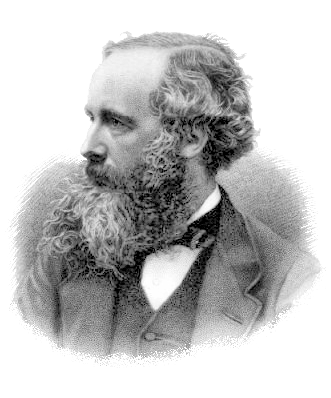
\includegraphics{James_Clerk_Maxwell.png}
    
\end{figure}

\begin{figure}[h]
    \centering     
    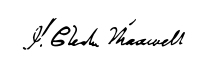
\includegraphics{James_Clerk_Maxwell_sig.png}
    
\end{figure}

\newpage 


\section{Equazioni di Maxwell nel vuoto} 

\footnote{Equazioni di Maxwell - Wikipedia}

Le equazioni di Maxwell sono le seguenti: \\ \\ 

{ \Large \begin{equation}
    \begin{cases}
        
\nabla \cdot \vec{D} = \rho \\ 

\nabla \cdot \vec{B} = 0 \\ 

\nabla \times \vec{E} = -\frac{\partial \vec{B}}{\partial t} \\

\nabla \times \vec{H} = \vec{J} + \frac{\partial \vec{D}}{\partial t}

    \end{cases}
\end{equation}}

\begin{tcolorbox}
    I vettori verranno indicati con la freccia sopra alla lettera del vettore stesso. \\ 
    Un elenco degli operatori matematici che troverai nel corso: \\ \\ 
    
    $\cdot$ Prodotto scalare \\ 
    $\times$ Prodoto vettoriale \\ 
    $\frac{\partial}{\partial t}$ Derivata nel tempo \\ 
    $\nabla$ Operatore nabla \\ 
    $\nabla \cdot$ Divergenza \\  
    $\nabla \times $ Rotore \\ 

    Per capire meglio perchè si usano questi operatori matematici in questo corso, puoi visualizzare questo video di \\\\  
    ClearMath - Rotore e Divergenza: Cosa sono? A che Servono? \\ 
    \url{https://youtu.be/q00XcRm7XBs?si=kWH6J1_2AyCfSYWB} \\\\ 
        
    Step by Step - Fisica e Mate - FISICA Teoria 4 tris - PRODOTTO SCALARE, PRODOTTO VETTORIALE, REGOLA della MANO DESTRA \\ 
    \url{https://youtu.be/MJZnMRb9yZ0?si=rgOIhrHFdt5DQf45} \\\\  


\end{tcolorbox}


Per un vettore F, possiamo visualizzare il rotore e la divergenza come: 


\begin{figure}[h]
    \centering
    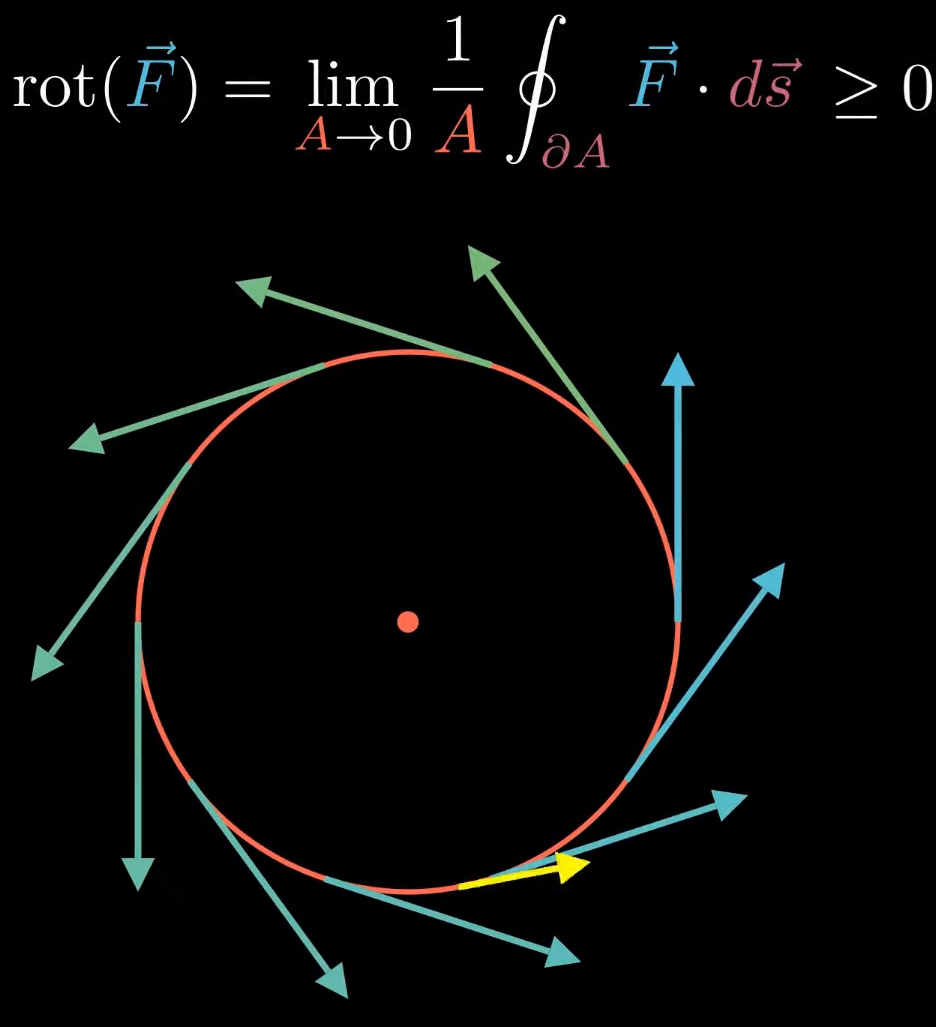
\includegraphics[scale= 0.2]{Rotore e Divergenza_ Cosa Sono_ A che Servono_ 1-36 screenshot.png}
    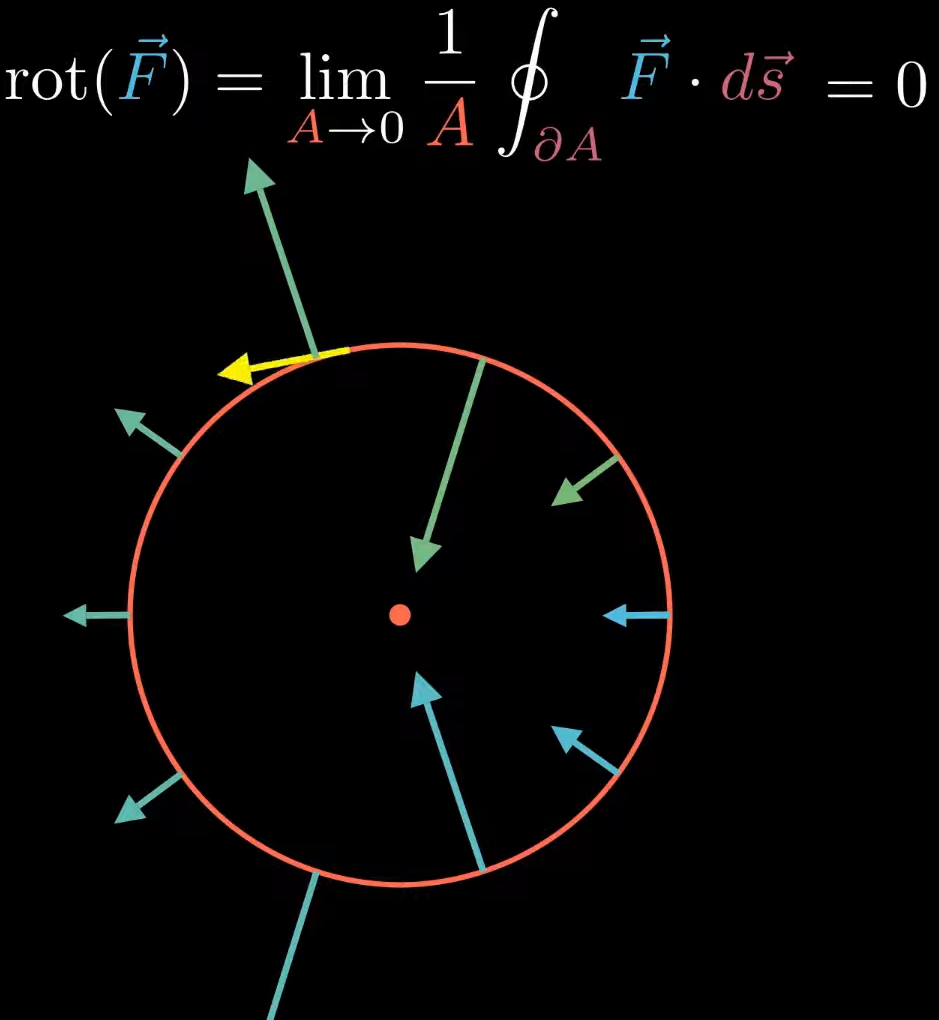
\includegraphics[scale= 0.2]{Rotore e Divergenza_ Cosa Sono_ A che Servono_ 2-10 screenshot.png}
    
\end{figure}

\begin{figure}[h]
    \centering
    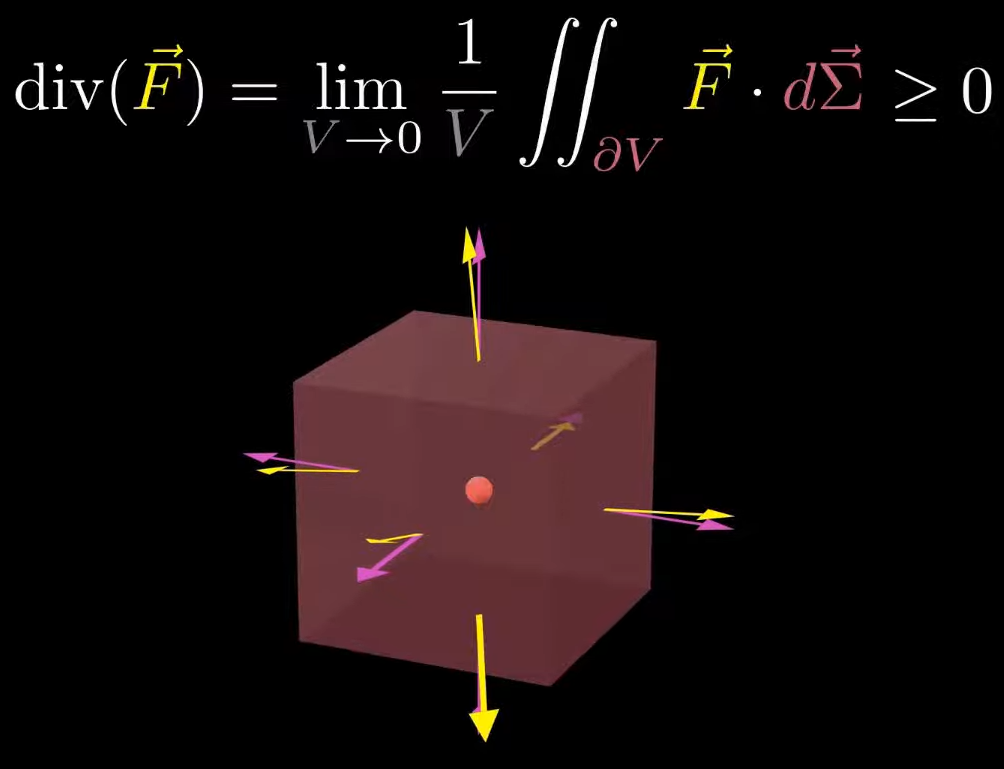
\includegraphics[scale= 0.2]{Rotore e Divergenza_ Cosa Sono_ A che Servono_ 6-43 screenshot.png}
    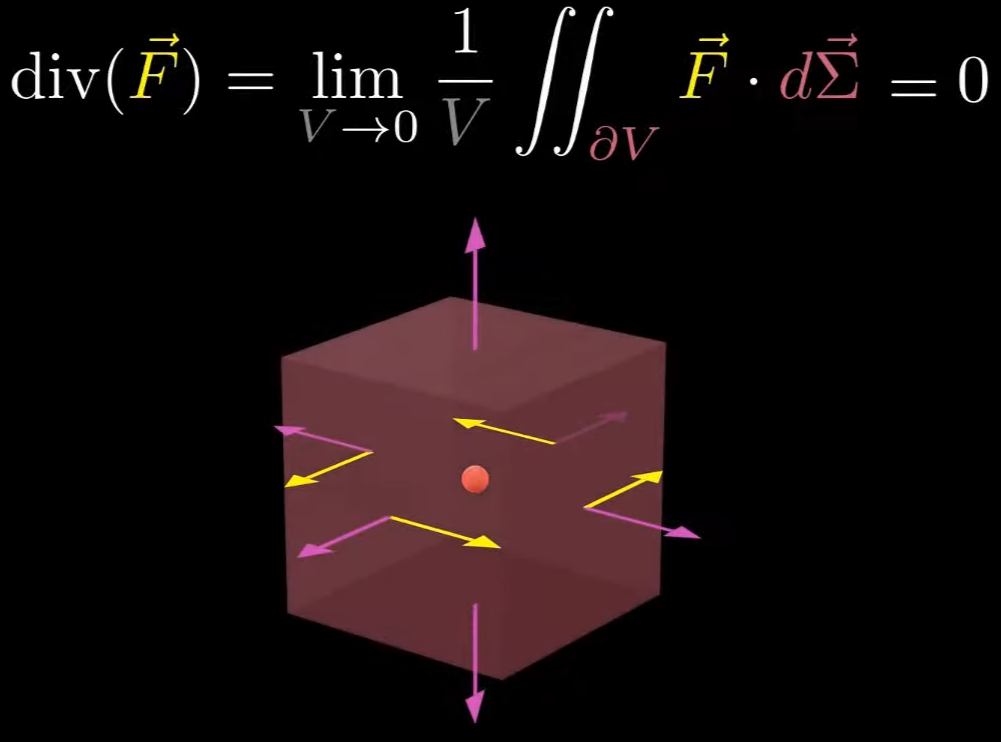
\includegraphics[scale= 0.2]{Rotore e Divergenza_ Cosa Sono_ A che Servono_ 7-6 screenshot.png}
    
\end{figure}

\begin{tcolorbox}
    Le foto sono degli screenshoot da \\
    ClearMath - Rotore e Divergenza: Cosa sono? A che Servono? \\ 
    \url{https://youtu.be/q00XcRm7XBs?si=kWH6J1_2AyCfSYWB} \\\\ 
     
    Da \url{https://it.wikipedia.org/wiki/Divergenza} \\ 
    la divergenza è un campo scalare che misura la tendenza di un campo vettoriale a divergere o a convergere verso un punto dello spazio. \\ 

    Da \url{https://it.wikipedia.org/wiki/Rotore_(matematica)} \\ 
    Il rotore esprime una rotazione infinitesima (ad esempio una velocità di rotazione) del vettore dato, associando a ogni punto dello spazio un vettore.
\end{tcolorbox}
\newpage

\subsection{Legenda - Equazioni di Maxwell nel vuoto}

$\vec{D}$ Flusso del campo elettrico \\ 
$\vec{E}$ Campo elettrico \\ 
$\vec{B}$ Flusso del campo magnetico \\ 
$\vec{H}$ Campo magnetico \\
$\vec{J}$ Densità di corrente \\ 
$\rho$ Densità di carica \\\\ 

\begin{tcolorbox}
    Adesso che sappiamo cosa sono e come si chiamano gli operatori matematici ed i vettori che ci servono, 
    possiamo leggere in italiano le formule matematiche date. \\ 
    
    $\nabla \cdot \vec{D} = \rho$ \\ 
    anche detta legge di Gauss elettrica, esprime che \\ 
    la divergenza del flusso del campo elettrico è uguale alla densità di carica \\ \\

    $\nabla \cdot \vec{B} = 0$ \\ 
    anche detta legge di Gauss magnetica, esprime che \\ 
    la divergenza del flusso del campo magnetico è uguale a zero \\ \\ 

    $\nabla \times \vec{E} = -\frac{\partial \vec{B}}{\partial t}$ \\
    anche detta legge di Faraday, esprime che \\ 
    il rotore del campo elettrico è uguale alla derivata nel tempo del flusso del campo magnetico, 
    con verso contrario rispetto al campo elettrico stesso \\ \\ 
    
    $\nabla \times \vec{H} = \vec{J} + \frac{\partial \vec{D}}{\partial t}$ \newline
    anche detta legge di Ampere-Maxwell, esprime che \\ 
    il rotore del campo magnetico è uguale alla somma della densità di corrente 
    e la derivata nel tempo del flusso del campo elettrico \\ \\ 



\end{tcolorbox}


\newpage 

\section{Equazioni di Maxwell nel vuoto in assenza di cariche} 
\footnote{FWC - pag 132 | 3.9 Maxwell's equations and plane waves}

In assenza di cariche, possiamo considerare: \\

{ \Large \begin{equation}
    \begin{cases}
    
        \rho = 0 \\ 
        \vec{J} = 0  

    \end{cases}
\end{equation}}

\begin{tcolorbox}

    $\rho = 0$ \\
    La densità di carica è uguale a zero \\ \\ 

    $\vec{J} = 0$\\ 
    La densità di corrente è uguale a zero 

\end{tcolorbox}


Quindi, le leggi di Maxwell diventeranno: \\ 


{  \Large \begin{equation}
    \begin{cases}
        \nabla \cdot \vec{D} = \rho \Rightarrow \nabla \cdot \vec{D} = 0  \\
        \nabla \times \vec{H} = \vec{J} + \frac{\partial \vec{D}}{\partial t} 
        \Rightarrow \nabla \times \vec{H} = \frac{\partial \vec{D}}{\partial t} \newline 
        
    \end{cases}
\end{equation}}

Per riassumere, le equazioni di Maxwell nel vuoto in assenza di cariche sono: 

{ \Large \begin{equation}
    \begin{cases}
    
        \nabla \cdot \vec{D} = 0 \\
        \nabla \cdot \vec{B} = 0 \\
        \nabla \times \vec{E} = -\frac{\partial \vec{B}}{\partial t} \\
        \nabla \times \vec{H} = \frac{\partial \vec{D}}{\partial t} \\ 

    \end{cases}
\end{equation}}

\begin{tcolorbox}
    
    $\nabla \cdot \vec{D} = 0$ \\
    La divergenza del flusso del campo elettrico è uguale a zero \\ \\ 

    $\nabla \cdot \vec{B} = 0$ \\
    La divergenza del flusso del campo magnetico è uguale a zero \\ \\ 

    $\nabla \times \vec{E} = -\frac{\partial \vec{B}}{\partial t}$ \\
    Il rotore del campo elettrico è uguale alla derivata nel tempo del flusso del campo magnetico, 
    con verso contrario rispetto al campo elettrico stesso \\ \\ 

    $\nabla \times \vec{H} = \frac{\partial \vec{D}}{\partial t}$ \\ 
    Il rotore del campo magnetico è uguale alla derivata nel tempo del flusso di campo elettrico 

\end{tcolorbox} 

\newpage 

\section{Equazioni di Maxwell nei materiali} 

\footnote{FWC - pag 126 | 3.6 Maxwell's equations in differntial form} 

In questa sezione, prenderemo in considerazione materiali lineari isotropici:
lineari perchè le grandezze del materiale sono lineari, 
isotropici perchè le caratteristiche del materiale 
sono uguali in ogni punto del materiale stesso. \\ 

Ponendo: 

{ \Large \begin{equation}
    \begin{cases}
        
        \varepsilon = \varepsilon_0 \varepsilon_r \\ 
        \mu = \mu_0 \mu_r 

    \end{cases}
\end{equation}} 

$\varepsilon_0$ è la costante dielettrica nel vuoto \\ 
$\varepsilon_r$ è il rapporto tra la costante dielelttrica nel materiale e $\varepsilon_0$ \\ 

$\mu_0$ è la costante di permeabilità nel vuoto \\ 
$\mu_r$ è il rapporto tra la costante di permeabilità nel materiale e $\mu_0$ \\ \\ 

Dalle leggi di Maxwell nel vuoto senza cariche, poniamo: 

{ \Large \begin{equation}
    \begin{cases}
        
        \vec{D} = \varepsilon \vec{E} \\ 
        \vec{B} = \mu \vec{H}

    \end{cases}
\end{equation}} 

\begin{tcolorbox}

    Nota matematica: \\  
    $\varepsilon \vec{E}$ è un prodotto scalare tra uno scalare (quindi un valore) e un vettore. \\ 
    Lo stesso principio vale per $\mu \vec{H}$ \\  

    Nota lettura italiano: \\ \\  
    $\vec{D} = \varepsilon \vec{E}$ \\ 
    Il flusso del campo elettrico è uguale alla costante dielettrica nel materiale per il campo elettrico \\ \\ 

    $\vec{B} = \mu \vec{H}$ \\ 
    Il flusso del campo magnetico è uguale alla costante magnetica nel materiale per il campo magentico 



\end{tcolorbox}


Svolgendo le dovute sostituzioni dalle leggi di Maxwell nel vuoto senza cariche, avremo che: \\ \\ 


{
    \Large 
    \begin{equation}
        \begin{cases}
         \nabla \cdot \vec{D} = 0 
\Rightarrow 
\nabla \cdot (\varepsilon \vec{E}) = 0
\Rightarrow
\nabla \cdot \frac{\varepsilon \vec{E}}{\varepsilon} = \frac{0}{\varepsilon}
\Rightarrow
\nabla \cdot \vec{E} = 0 \\
\nabla \cdot \vec{B} = 0 
\Rightarrow
\nabla \cdot (\mu \vec{H}) = 0
\Rightarrow
\nabla \cdot \frac{\mu \vec{H}}{\mu} = \frac{0}{\mu}
\Rightarrow
\nabla \cdot \vec{H} = 0 \\ 
\nabla \times \vec{E} = -\frac{\partial \vec{B}}{\partial t}
\Rightarrow
\nabla \times \vec{E} = -\frac{\partial (\mu \vec{H} )}{\partial t}
\Rightarrow
\nabla \times \vec{E} = -\mu \frac{\partial \vec{H}}{\partial t}\\ 
\nabla \times \vec{H} = \frac{\partial \vec{D}}{\partial t}
\Rightarrow
\nabla \times \vec{H} = \frac{\partial (\varepsilon \vec{E})}{\partial t}
\Rightarrow
\nabla \times \vec{H} = \varepsilon \frac{\partial \vec{E}}{\partial t}   
        \end{cases}
    \end{equation}
}

Per riassumere, le equazioni di Maxwell nei materiali, in assenza di cariche, sono: 

{ \Large \begin{equation}
    \begin{cases}
        
        \nabla \cdot \vec{E} = 0 \\ \\ 
        \nabla \cdot \vec{H} = 0 \\ \\ 
        \nabla \times \vec{E} = -\mu \frac{\partial \vec{H}}{\partial t} \\ \\ 
        \nabla \times \vec{H} = \varepsilon \frac{\partial \vec{E}}{\partial t} 


    \end{cases}
\end{equation}} 

\begin{tcolorbox}
    $\nabla \cdot \vec{E} = 0 $\\ 
    La divergenza del campo elettrico è uguale a zero \\ \\ 

    $\nabla \cdot \vec{H} = 0$ \\
    La divergenza del campo magnetico è uguale a zero \\ \\ 
    
    $\nabla \times \vec{E} = -\mu \frac{\partial \vec{H}}{\partial t}$ \\  
    Il rotore del campo elettrico è uguale al prodotto tra la derivata del campo magnetico nel tempo per la costante di permeabilità 
    nel materiale con segno opposto rispetto al campo elettrico \\ \\ 

    $\nabla \times \vec{H} = \varepsilon \frac{\partial \vec{E}}{\partial t}$ \\ 
    Il rotore del campo magnetico è uguale al prodotto tra la derivata nel tempo del campo elettrico e la costante elettrica nel materiale



\end{tcolorbox} 

\newpage 
\section{Equazioni di Maxwell nelle coordinate cartesiane} 

\footnote{FWC - pag 85 | 2.5 The curl of a  vector field \\ FWC - pag 132 | 3.9 Maxwell's equations and plane waves } 


Considerando il sistema delle coordinte cartesiane, cioè un sistema in cui ogni punto ha coordinate (x,y,z) , possiamo scrivere che: \\ 

{
    \Large 
    \begin{equation}
 \nabla = (\frac{\partial}{\partial x} , \frac{\partial}{\partial y} , \frac{\partial}{\partial z})
    \end{equation}
}

Quindi: \\ 

{
    \Large
    \begin{equation}
        \nabla \times \vec{E} = \operatorname{rot} 
\begin{vmatrix}
    \hat{x} & \hat{y} &\hat{z} \\ \\ 
    \frac{\partial}{\partial x} & \frac{\partial}{\partial y} & \frac{\partial}{\partial z} \\ \\ 
    E_x & E_y & E_z
\end{vmatrix}  
    \end{equation}
}

$\hat{x} , \hat{y} , \hat{z}$ sono i versori delle coordinate cartesiane, cioè i vettori unitari del sistema cartesiano. \\ 
$E_x , E_y , E_z$ sono le ampiezze di $\vec{E}$ nei rispettivi assi cartesiani \\ 

%Vedi appunti%

Ora andiamo a calcalore il rotore di $\vec{E}$ 

\begin{tcolorbox}
    A livello operativo, calocare il rotore di un vettore significa calcolare il determinante della matrice 
    $\begin{vmatrix}
        \hat{x} & \hat{y} &\hat{z} \\ \\ 
        \frac{\partial}{\partial x} & \frac{\partial}{\partial y} & \frac{\partial}{\partial z} \\ \\ 
        E_x & E_y & E_z
    \end{vmatrix} $ \\ \\ 

    Se non sai calcolare il determinante di una matrice, ti consiglio questo video: \\ \\ Elia Bombardelli - Determinante di una Matrice  \\ \url{https://youtu.be/pstBLN4gCqE?si=pkqB5MmdOgCFapP9} 
\end{tcolorbox}

Svolgendo i calcoli passo-passo, avremo che: \\ 

{
    \Large
    \begin{equation}
        \begin{split}
        \nabla \times \vec{E} 
        &= \operatorname{rot} 
\begin{vmatrix}
    \hat{x} & \hat{y} &\hat{z} \\ \\ 
    \frac{\partial}{\partial x} & \frac{\partial}{\partial y} & \frac{\partial}{\partial z} \\ \\ 
    E_x & E_y & E_z
\end{vmatrix}  \\ \\
&= \hat{x} 
\begin{vmatrix}
    \frac{\partial}{\partial y} & \frac{\partial}{\partial z} \\  \\ 
    E_y & E_z 
\end{vmatrix}  
- \hat{y} 
\begin{vmatrix}
    \frac{\partial}{\partial x} & \frac{\partial}{\partial z} \\  \\ 
    E_x & E_z 
\end{vmatrix} 
+ \hat{z} 
\begin{vmatrix}
    \frac{\partial}{\partial x} & \frac{\partial}{\partial y} \\  \\ 
    E_x & E_y 
\end{vmatrix} \\ \\
&= \hat{x} (\frac{\partial E_z}{\partial y} - \frac{\partial E_y}{\partial z})
 - \hat{y} (\frac{\partial E_z}{\partial x} - \frac{\partial E_x}{\partial z})
 + \hat{z} (\frac{\partial E_y}{\partial x} - \frac{\partial E_x}{\partial y}) \\ \\
&= \hat{x} (\frac{\partial E_z}{\partial y} - \frac{\partial E_y}{\partial z})
 + \hat{y} (-\frac{\partial E_z}{\partial x} + \frac{\partial E_x}{\partial z})
 + \hat{z} (\frac{\partial E_y}{\partial x} - \frac{\partial E_x}{\partial y})
        \end{split}
    \end{equation}
}

Possiamo svolgere gli stessi passaggi svolti anche per $\nabla \times \vec{H}$ \\

{
    \Large
    \begin{equation}
\nabla \times \vec{H} 
= \hat{x} (\frac{\partial H_z}{\partial y} - \frac{\partial H_y}{\partial z})
+ \hat{y} (-\frac{\partial H_z}{\partial x} + \frac{\partial H_x}{\partial z})
+ \hat{z} (\frac{\partial H_y}{\partial x} - \frac{\partial H_x}{\partial y})
    \end{equation}
}

Per riassumere, le equazioni di Maxwell nei materiali nelle coordinate cartesiane sono le seguenti: \\ 

{ \Large \begin{equation}
    \begin{cases}
        \nabla \cdot \vec{E} = 0 \\ \\ 
        \nabla \cdot \vec{H} = 0 \\ \\
        
        \nabla \times \vec{E} 
        = \hat{x} (\frac{\partial E_z}{\partial y} - \frac{\partial E_y}{\partial z})
        + \hat{y} (-\frac{\partial E_z}{\partial x} + \frac{\partial E_x}{\partial z})
        + \hat{z} (\frac{\partial E_y}{\partial x} - \frac{\partial E_x}{\partial y}) \\ \\ 


        \nabla \times \vec{H}  
 = \hat{x} (\frac{\partial H_z}{\partial y} - \frac{\partial H_y}{\partial z})
 + \hat{y} (-\frac{\partial H_z}{\partial x} + \frac{\partial H_x}{\partial z})
 + \hat{z} (\frac{\partial H_y}{\partial x} - \frac{\partial H_x}{\partial y}) \\ 


 
    \end{cases}
\end{equation}} 

\newpage 

\section{Equazioni di Maxwell per le onde piane in (x, y, z)}
\footnote{FWC - pag 132 | 3.9 Maxwell's equations and plane waves }


Considerando le onde piane, cioè onde in cui il fronte d'onda è infinito, possiamo calcolarci le equazioni di Maxwell per questo 
tipo d'onda. \\ 

Le onde piane, nella realtà, non esistono, ma ci sono utili per modellare le onde reali e per semplificarci i conti:
da sei incognite delle equazioni di Maxwell trovate nella sezione precedente, passeremo a due, cioè $E_x$ e $E_y$. \\ 
Gli altri componenti del campo elettromagnetico dipenderanno da queste due variabili indipendenti. \\ 


Ricordando che il fronte d'onda è infinito, 
le onde piane sono onde per cui non c'è variazione dell'onda lungo l'asse x e lungo l'asse y, quindi possiamo scrivere: 

{ \Large \begin{equation}
    \begin{cases}
        \frac{\partial}{\partial x} = 0 \\ \\  
        \frac{\partial}{\partial y} = 0 \\ 
        
    \end{cases}
\end{equation}}

$\nabla \times \vec{E}$ da: 

{
    \Large
    \begin{equation}
        \nabla \times \vec{E} 
        = \hat{x} (\frac{\partial E_z}{\partial y} - \frac{\partial E_y}{\partial z})
        + \hat{y} (-\frac{\partial E_z}{\partial x} + \frac{\partial E_x}{\partial z})
        + \hat{z} (\frac{\partial E_y}{\partial x} - \frac{\partial E_x}{\partial y}) 
    \end{equation}
}

diventa: 

{
    \Large 
    \begin{equation}
        \nabla \times \vec{E} = \hat{x} (- \frac{\partial E_y}{\partial z})
+ \hat{y} (\frac{\partial E_x}{\partial z})
+ \hat{z} (0)  
    \end{equation}
}

Dalle leggi di Maxwell nei materiali, sappiamo che:  

{
    \Large 
    \begin{equation}
        \nabla \times \vec{E} = - \mu \frac{\partial \vec{H}}{\partial t}   
    \end{equation}
}

Scomponendo questa equazione nei vari assi cartesiani, avremo che: \\ \\ 

\textbf{Asse X} 
{
    \Large
    \begin{equation}
     -\frac{\partial E_y}{\partial z} = -\mu \frac{\partial H_x}{\partial t}   
    \end{equation}
}

\textbf{Asse Y}  

{
    \Large
    \begin{equation}
        \frac{\partial E_x}{\partial z} = -\mu \frac{\partial H_y}{\partial t}  
    \end{equation}
}

\textbf{Asse Z}  

{
    \Large 
    \begin{equation}
        0 = -\mu \frac{\partial H_z}{\partial t}   
    \end{equation}
}

Quello che abbiamo fatto per $\nabla \times \vec{E}$, possiamo farlo anche per $\nabla \times \vec{H}$ \\ 

{
    \Large
    \begin{equation}
     \nabla \times \vec{H} = \varepsilon \frac{\partial \vec{E}}{\partial t}   
    \end{equation}
}
Scomponendo questa equazione nei vari assi cartesiani, avremo che: \\ \\ 

\textbf{Asse X} 
{
    \Large 
    \begin{equation}
    -\frac{\partial H_y}{\partial z} = \varepsilon \frac{\partial E_x}{\partial t}   
    \end{equation}
}

\textbf{Asse Y} 
{
    \Large 
    \begin{equation}
     \frac{\partial H_x}{\partial z} = \varepsilon \frac{\partial E_y}{\partial t}   
    \end{equation}
}


\textbf{Asse Z} 
{
    \Large
    \begin{equation}
        0 = \varepsilon \frac{\partial E_z}{\partial t}    
    \end{equation}
}

\begin{tcolorbox}
    Scriverò un esempio che può essere applicato per tutte le altre eqazioni. \\ \\ 
    $\frac{\partial H_x}{\partial z} = \varepsilon \frac{\partial E_y}{\partial t}$ \\ 

    La derivata per z della componente sull'asse x del campo magnetico è uguale al prodotto tra la costante elettrica nel materiale e la derivata 
    nel tempo della componente sull'asse y del campo elettrico 

\end{tcolorbox}

Considerando le equazioni sull'asse z, abbiamo che: \\ 

{ \Large \begin{equation}
    \begin{cases}
        \varepsilon \frac{\partial E_z}{\partial t} = 0 \\
        -\mu \frac{\partial H_z}{\partial t} = 0 
    \end{cases} 
    \Rightarrow
    \begin{cases}
        E_z = 0\\
        H_z = 0 
    \end{cases}
\end{equation}} \\ 

Queste equazioni ci dicono che i campi sono trasversali rispetto alla direzione di propagazione (considerando 
l'asse z come asse di propagazione)

\begin{tcolorbox}
    Da \url{https://it.wikipedia.org/wiki/Onda_trasversale} \\
    Un' onda trasversale è un'onda in movimento che è composta da oscillazioni che avvengono perpendicolari alla direzione del trasferimento di energia. Se un'onda trasversale si muove nella direzione positiva x, le sue oscillazioni sono nelle direzioni sopra e sotto che giacciono nel piano y-z.
\end{tcolorbox}

Questo significa che $\vec{E}$ e $\vec{H}$ sono perpendicolari. 

Analizzando le altre equazioni nel piano (x,y), notiamo che: 

{ \Large \begin{equation}
    \begin{cases}
        \frac{\partial E_x}{\partial z} = -\mu \frac{\partial H_y}{\partial t} \\
        -\frac{\partial H_y}{\partial z} = \varepsilon \frac{\partial E_x}{\partial t} 

    \end{cases}
\end{equation}} \\ 

Possiamo risolvere questo sistema per $E_x$ \\ 

Differenziando per $\frac{\partial}{\partial z}$ nella prima equazione e $\frac{\partial}{\partial t}$ 
nella seconda equazione, avremo che: 

{ \Large \begin{equation}
    \begin{cases}
        \pdv[2]{E_x}{z} = - \mu \pdv{H_y}{t}{z} \\ \\  
        \pdv[2]{H_y}{z}{t} = - \mu \pdv{E_y}{t} \\ 
        
    \end{cases}
\end{equation}} \\ 

Sostituendo la seconda equazione alla prima, abbiamo che: \\ \\ 

{
    \Large 
    \begin{equation}
        \pdv[2]{E_x}{z} = \mu \varepsilon \pdv[2]{E_x}{t}   
    \end{equation}
}

Questa indicata è l'equazione dell'onda a una dimensione lunga la direzione z. 

Lo stesso procedimento svolto per trovare $E_x$, lo possiamo usare con $E_y$ \\ 

L'onda si propaga con velocità: \\ \\ 

{
    \Large
    \begin{equation}
        v = \frac{1}{\sqrt{\mu \varepsilon}}
    \end{equation}
}

\begin{tcolorbox}
    Per vedere un altro punto di vista dell'equazione dell'onda, puoi visualizzare questo video di \\ \\
    Ali the Dazzling - The Wave Equation simplified \\ 
    \url{https://youtu.be/tGc4gb8n7gM?si=H4Jw0vzIKAW2jeqv} \\ 

    Putroppo è in inglese e non ha i sottotitoli in italiano, ma il video è molto semplice e molto intuitivo 
\end{tcolorbox}

\newpage 

\section{Equazioni di Maxwell in forma fasoriale}
\footnote{FWC - pag 135 | 3.10 Uniform plane waves with steady-state sinusoids}

Oltre alle onde piane negli assi cartesiani, è possibile esprimere le onde usando i fasori. 

\begin{tcolorbox}
    Se non sai cosa è un fasore, puoi visualizzare questo video di \\ \\ 
    Elettronica-mente - Elettrotecnica - Lezione 15 - Fasori, Impedenza ed Ammettanza \\ 
    \url{https://youtu.be/_Yww5MfoPwI?si=7e-8G0q_gUFOcTev} 

\end{tcolorbox}

Ponendo: 
{
    \Large
    \begin{equation}
    \frac{\partial}{\partial t} = \jmath \omega   
    \end{equation}
}

possiamo riscrivere le equazioni di Maxwell nei materiali come: \\   

{ \Large \begin{equation}
    \begin{cases}
        \nabla \cdot \vec{D} = 0 \\
        \nabla \cdot \vec{B} = 0 \\
        \nabla \times \vec{E} = -\mu \frac{\partial \vec{H}}{\partial t} \\
        \nabla \times \vec{H} = \varepsilon \frac{\partial \vec{E}}{\partial t}  

    \end{cases} 
    \Rightarrow
    \begin{cases}
        \nabla \cdot \vec{D} = 0 \\
        \nabla \cdot \vec{B} = 0 \\
        \nabla \times \vec{E} = - \jmath \omega \mu \vec{H} \\
        \nabla \times \vec{H} = \jmath \omega \varepsilon \vec{E}  

    \end{cases}
\end{equation}} \\ 


Per lo stesso principio, possiamo scrivere le sue componenti lungo (x,y, z) come: \\ 

{
    \Large 
    \begin{equation}
    \nabla \times \vec{E} = - \jmath \omega \mu \vec{H}    
    \end{equation}
}

\textbf{Asse X} 

{
    \Large 
    \begin{equation}      
-\frac{\partial E_y}{\partial z} = -\jmath \omega \mu H_x 
    \end{equation}
}

\textbf{Asse Y}  
{
    \Large
    \begin{equation}
\frac{\partial E_x}{\partial z} = - \jmath \omega \mu H_y    
    \end{equation}
}

\textbf{Asse Z} 
{
    \Large
    \begin{equation}
        0 = \jmath \omega \mu H_z   
    \end{equation}
}

Invece per: 

{
    \Large
    \begin{equation}
    \nabla \times \vec{H} = \jmath \omega \varepsilon \vec{E} 
    \end{equation}
}

\textbf{Asse X} 
{
    \Large 
    \begin{equation}
        -\frac{\partial H_y}{\partial z} = \jmath \omega \varepsilon E_x   
    \end{equation}
} 


\textbf{Asse Y} 
{
    \Large
    \begin{equation}
    \frac{\partial H_x}{\partial z} = \jmath \omega \varepsilon E_y   
    \end{equation}
}

\textbf{Asse Z} 

{
    \Large
    \begin{equation}
    0 = \jmath \omega \varepsilon E_z  
    \end{equation}
}
L'equazione dell'onda, in forma fasoriale, diventa: \\ 

{
    \Large
    \begin{equation}
    \pdv[2]{E_x}{z} = - \omega ^ 2 \mu \varepsilon E_x   
    \end{equation}
}

in cui 

{
    \Large
    \begin{equation}
        \pdv[2]{}{t} = - \omega ^ 2   
    \end{equation}
}
in forma fasoriale. 

Come il caso delle equazione di Maxwell delle onde onde piane nei materiali, 
{
    \Large
    \begin{equation}
E_z = H_z = 0 
    \end{equation}
}
\newpage 










\chapter{Onde in forma fasoriale} 

\begin{figure}[h]
    \centering
    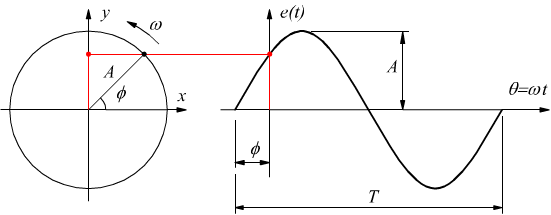
\includegraphics[scale = 0.9]{Fasori rappresentazione.png}
    
\end{figure}

\newpage 

\section{Equazioni dell'onda in forma fasoriale}

\footnote{FWC - pag 135 | 3.10 Uniform plane waves with steady-state sinusoids } 

Prendiamo una componente del campo elettrico, ad esempio $E_x (z,t)$. \\ 
Essenndo una sinusoide, $E_x (z,t)$ possiamo scriverla nella forma: 

{\Large \begin{equation}
    E_x (z,t) = C_1 e^{-\jmath \kappa z} + C_2 e^{\jmath \kappa z}
\end{equation}} 

in cui: 

\begin{itemize}
    \item $C_1$ e $C_2$ sono numeri reali 
    \item $C_1 = E_o ^+  $
    \item $C_2 = E_o ^-  $  
    \item $\kappa = \omega \sqrt{\mu \varepsilon} = \frac{\omega}{v}$
\end{itemize} 

\begin{tcolorbox}
    Dalla matematica, 
    $\omega$ (si legge omega) è la frequenza dell'onda misurata in radianti al secondo [rad/s]. \\ 
    $\omega = 2\pi f$ \\ 
    dove f è la frequenza dell'onda o l'inverso di un periodo misurata in [Hz] (si legge Hertz) o [$\frac{1}{s}$].  \\ \\ 
    
    $\jmath$ è l'unità immaginaria. \\ 
    $\jmath^{2} = -1$ \\ \\ 

    è il numero di Eulero. \\  



    Perchè scrivere le onde in forma fasoriale? \\ \\ 
    Tutto grazie alla formula di Eulero: \\ \\ 
    $e^{\jmath z} = \cos(z) + \jmath \sin(z)$ \\ \\

    Se vuoi approfondire, ci sono due video molto interessanti riguardo al tema: 

    \begin{itemize}
        \item Zech Star - Why do Electrical Engineers use imaginary numbers in circuit analysis? \\ \url{https://youtu.be/FCNHN7B9iDM?si=9ECin22SXTxcp7-6} 
        \item The Science Asylum - What the HECK is a Phasor? Alternating Current Explained. \\ \url{https://youtu.be/7weMCsff0xw?si=Y9t8nKBIX3a1I5Z5}
    \end{itemize}

    

\end{tcolorbox}

$\kappa$ prende il nome di numero d'onda o costante di fase e si misura in $[\frac{1}{m}]$; può essere vista 
anche come la costante del medio per una particolare frequenza (ricordando che $\mu$ e $\varepsilon$ dipendono rispettivamente da $\mu_r$ 
e $\varepsilon_r$ del materiale) \\ 

$E_x (z,t)$ è una funzione che dipende sia da z (nell'asse cartesiano) che da t (cioè il tempo).  \\ \\

Essa è la somma di un'onda progressiva, cioè un'onda lungo z, che viene indicata dalla notazione $E_o ^+ e^{-\jmath \kappa z}$ 
e di un'onda regressiva, cioè un'onda lungo -z, che viene indicata dalla notazione $E_o ^- e^{\jmath \kappa z}$ \\ 

$E_o ^+ e^{-\jmath \kappa z}$ diventa negativa lungo l'asse z, con velocità v, mentre $E_o ^- e^{\jmath \kappa z}$ dievnta positiva 
lungo l'asse -z con velocità -v. \\ \\ 

Moltiplicando l'equazione per $e^{\jmath \omega t}$, è possibile convertirla in coordinate cartesiane e sapere come l'onda varia nel tempo:

{
    \Large
    \begin{equation}
        \begin{split}
            E_x (z,t) 
            &= \mathfrak{Re}[E_x e^{\jmath \omega t}]\\ 
            &= \mathfrak{Re}[C_1 e^{- \jmath \kappa z} e^{\jmath \omega t} +  C_2 e^{ \jmath \kappa z} e^{\jmath \omega t}]            
        \end{split}
    \end{equation}
}


Prendendo $C_1$ e $C_2$ come reali, avremo che: 

{
    \Large
    \begin{equation}
    E_x (z,t) = C_1 \cos(\omega t - \kappa z) + C_2 \cos(\omega t + \kappa z)    
    \end{equation}
}

Ricordando che: 
{
    \Large
    \begin{equation}
        \kappa = \frac{\omega}{v}   
    \end{equation}
}

possiamo scriverla anche come: 
{
    \Large 
    \begin{equation}
    E_x (z,t) = C_1 \cos\omega( t - \frac{z}{v}) + C_2 \cos\omega( t + \frac{z}{v})
    \end{equation}
}

Nello scorso capitolo, le equazioni di Maxwell in forma fasoriale, abbiamo scoperto che:  
{
    \Large
    \begin{equation}
     \nabla \times \vec{E} = -\jmath \omega \mu \vec{H}   
    \end{equation}
}


Nell'asse y sappiamo la relazione tra $E_x$ e $H_y$:  

{
    \Large
    \begin{equation}
    \frac{\partial E_x}{\partial z} = -\jmath \omega \mu H_y     
    \end{equation}
}

Dividendo l'equazione per $-\jmath \omega \mu$, possiamo trovare $H_y$: 
{
    \Large
    \begin{equation}
   H_y = - \frac{1}{\jmath \omega \mu} \frac{\partial E_x}{\partial z }     
    \end{equation}
}

Ricordando che: 

{
    \Large
    \begin{equation}
   E_x (z,t) = C_1 e^{-\jmath \kappa z} + C_2 e^{\jmath \kappa z}     
    \end{equation}
}


$H_y$ possiamo scriverla come: 

{
    \Large
    \begin{equation}
   H_y = \frac{\kappa}{\omega \mu} [E_o ^+ e^{-\jmath \kappa z} - E_o ^- e^{\jmath \kappa z}]     
    \end{equation}
}

Sviluppando l'equazione, avremo che: 
{
    \Large 
    \begin{equation}
   H_y = \sqrt{\frac{\varepsilon}{\mu}} [E_o ^+ e^{-\jmath \kappa z} - E_o ^- e^{\jmath \kappa z}]      
    \end{equation}
}


In forma instantanea, $H_y$ la possiamo scrivere come: \\ 

{
    \Large
    \begin{equation} 
        \begin{split}
            H_y (z, t) 
            &= \mathfrak{Re}[H_y(z) e^{\jmath \omega t}] 
            \\
            &= \frac{1}{\sqrt{\frac{\mu}{\varepsilon}}}[E_o^+ \cos(\omega t - \kappa z) - E_o^- \cos(\omega t + \kappa z)]  
        \end{split}
    \end{equation}
}
dove: 

{
    \Large
    \begin{equation}
        \sqrt{\frac{\mu}{\varepsilon}} = \eta     
    \end{equation}
}

$\eta$ (si legge eta) prende il nome di impedenza d'onda. \\ \\ 

Ritornando all'esempio nel piano in z=0, \\ \\ 

{\Large \begin{equation}
    \begin{cases}
        E_x (z) = -2 \jmath E_0^+ \sin(\kappa z) \\ \\ 
        H_y (z) = 2 \frac{E_0^+}{\eta} \cos(\kappa z)
    \end{cases}
\end{equation}} \\ 

Da queste due equazioni finali, notiamo che $E_x (z)$ e $H_y (z)$ sono in quadratura 
di fase, cioè sono sfasati di 90° \\ \\ 

\begin{figure}[h]
    \centering 
    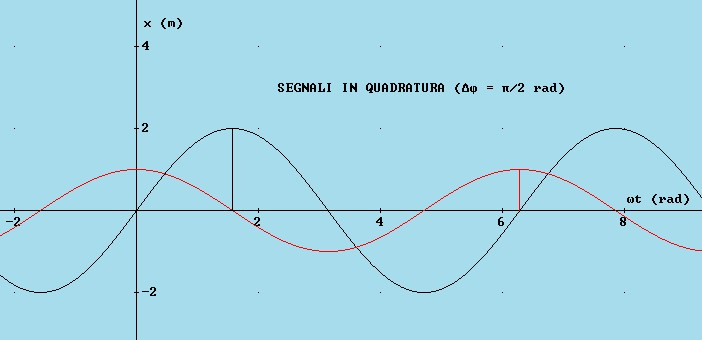
\includegraphics[scale = 0.8]{InQuadratura.jpg} 
    
\end{figure} 

\footnote{Wikipedia - Fase (Fisica)} \\ 

Per riassumere, usando le leggi di Maxwell per le onde piane, possiamo scriverle anche come: \\ 

{\Large \begin{equation}
    \begin{cases}
        \nabla ^{2} \vec{E} = -\kappa ^{2} \vec{E} \\ 
        \nabla ^{2} \vec{H} = -\kappa ^{2} \vec{H}
    \end{cases}
\end{equation}} 

dove: 
{
    \Large
    \begin{equation}
    \kappa ^{2} = \omega ^{2} \mu \varepsilon    
    \end{equation}
}

\newpage 









\chapter{Teorema di Poynting} 

\begin{figure}[h]
    \centering
    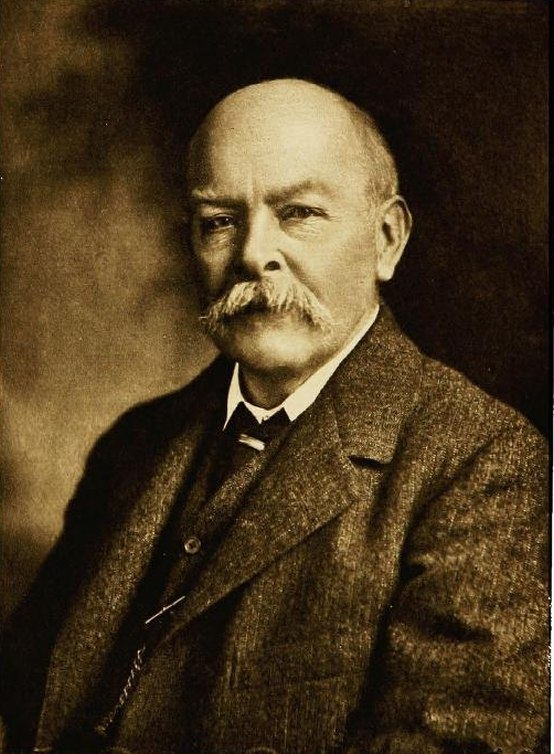
\includegraphics[scale = 0.5]{John_Henry_Poynting.jpg}
\end{figure} 

\begin{figure}[h]
    \centering 
    
\includegraphics[scale = 0.2]{John_Henry_Poynting_signature.png}
\end{figure} 

\newpage 

\section{Teorema di Poynting} 

\footnote{FWC - pag 139 | 3.12 Power flow in electromagnetic fields: Poynting's theorem }

Le onde elettromagnetiche possono portare energia. \\ 

Partendo dalle leggi di Maxwell generali: \\ 

{\Large \begin{equation}
    \begin{cases}
        \nabla \times \vec{E} = - \frac{\partial \vec{B}}{\partial t} \\ 
        \nabla \times \vec{H} = \vec{J} + \frac{\partial \vec{D}}{\partial t}
    \end{cases}
\end{equation}}

Ricordando anche che: \\ 

{\Large \begin{equation}
    \begin{cases}
        \vec{D} = \varepsilon\vec{E} \\ 
        \vec{B} = \mu \vec{H} 
    \end{cases}
\end{equation}} 

Possiamo scrivere, applicando la proprietà dei vettori: 

{
    \Large
    \begin{equation}
    \nabla \cdot (\vec{E} \times \vec{H}) = \vec{H} \cdot (\nabla \times \vec{E}) - \vec{E} \cdot (\nabla \times \vec{H})     
    \end{equation}
}

\begin{tcolorbox}
    Per approfondire questa proprietà vettoriale, puoi consultare questa pagina sul prodotto misto \\
    \url{https://it.wikipedia.org/wiki/Prodotto_misto}
\end{tcolorbox}

Sviluppando i prodotti vettoriali, avremo:  

{
    \Large
    \begin{equation}
    \nabla \cdot (\vec{E} \times \vec{H}) = - \vec{H} \cdot \frac{\partial \vec{B}}{\partial t} - \vec{E} \cdot \frac{\partial \vec{D}}{\partial t} - \vec{E} \cdot \vec{J}       
    \end{equation}
}

Da forma vettoriale a forma integrale: 

{
    \Large
    \begin{equation}
        - \int_V \nabla \cdot (\vec{E} \times \vec{H}) dV = 
        \int_V (\vec{H} \cdot \frac{\partial \vec{B}}{\partial t} + \vec{E} \cdot \frac{\partial \vec{D}}{\partial t} + \vec{E} \cdot \vec{J}) dV
    \end{equation}
}

\begin{tcolorbox}
    
    $\int_V dV$ si chiama integrale di un volume. È come l'integrale visto in analisi matematica 1 a una dimensione, 
    ma applicato in un volume. È un argomento di analisi matematica 2 \\   
    
    Per approfondire questo argomento,  consiglio questo video di \\ \\ 
    Clear Math -  Dall'astratto alla Realtà: guida completa sugli Integrali Tripli per Analisi 2 \\ 
    \url{https://youtu.be/4pDVpcJmnfY?si=pyKpC62rKZrk-i3L} \\ 

    Inoltre, se vuoi capire come siamo passati dalla forma vettoriale $\nabla \cdot (\vec{E} \times \vec{H})$ 
    alla forma integrale $- \int_V \nabla \cdot (\vec{E} \times \vec{H}) dV$, consiglio di vedere questo video 
    sul Teorema di Stokes:  \\ \\ 
    Clear Math - Devi saper fare questo esercizio sul Teorema di Stokes se vuoi passare Analisi 2 \\ 
    \url{https://youtu.be/-r8Er68ZOFk?si=8XxzHIWmG_z9Hl79}

    
    
\end{tcolorbox} 

Dal Teorema della divergenza, sappiamo che, dato un vettore $\vec{F}$: \\ 

{
    \Large 
    \begin{equation}
    \int_V \nabla \cdot \vec{F} dV = \oint_S \vec{F} \cdot \vec{dS}       
    \end{equation}
}

dove $\oint_S \vec{F} \cdot \vec{dS}$ è un integrale di linea lungo una superficie chiusa. \\ \\ 

Quindi, applicando il Teorema della divergenza, possiamo scrivere la precedente equzione come: \\ 

{
    \Large
    \begin{equation}
    - \oint_S (\vec{E} \times \vec{H}) \cdot \vec{dS} = \int_V  (\vec{H} \cdot \frac{\partial \vec{B}}{\partial t} + \vec{E} \cdot \frac{\partial \vec{D}}{\partial t} + \vec{E} \cdot \vec{J}) dV     
    \end{equation}
}

Quest'ultima equazione è il teorema di Poynting per qualsiasi mezzo. \\

Per mezzi lineari che non cambiano nel tempo, il teorema di Poynting lo possiamo scrivere in questa forma: 
{
    \Large
    \begin{equation}
    - \oint_S (\vec{E} \times \vec{H}) \cdot \vec{dS} = \int_V [\frac{\partial}{\partial t} (\frac{\vec{B} \cdot \vec{H}}{2}) + \frac{\partial}{\partial t} (\frac{\vec{D} \cdot \vec{E}}{2}) + \vec{E} \cdot \vec{J} ] dV       
    \end{equation}
}

Sostituendo dalla definizione di $\vec{D}$ e $\vec{B}$ per mezzi lineari in assenza di cariche: 
{
    \Large
    \begin{equation}
        \begin{cases}
\vec{D} = \varepsilon \vec{E}\\ 
\vec{B} = \mu \vec{H}         
        \end{cases}
    \end{equation}
}

L'equazione precedente diventa: 
{
    \Large
    \begin{equation}
    - \oint_S (\vec{E} \times \vec{H}) \cdot \vec{dS} = \int_V \vec{E} \cdot \vec{J} dV + \frac{1}{2} \frac{\partial}{\partial t} [\int_V \varepsilon \left| E \right| ^{2} dV + \int_V \mu \left| H \right| ^{2} dV ]        
    \end{equation}
} 

\begin{tcolorbox}
    $\left| E \right|$ e $\left| H \right|$ rappresentano il modulo, detta anche lunghezza , rispettivamente, del vettore $\vec{E}$ e del vettore $\vec{H}$ \\
    Per approfondire \url{https://www.youmath.it/lezioni/algebra-lineare/matrici-e-vettori/691-vettori-e-versori.html}
\end{tcolorbox} 

Quindi, $- \oint_S (\vec{E} \times \vec{H}) \cdot \vec{dS} $ rappresenta l'energia che entra in un volume per unità di tempo. \\ \\
In notazione matematica: 
{   
    \Large
    \begin{equation}
    W = \oint_S \vec{P} \cdot \vec{dS}      
    \end{equation}
}

dove: 

{   
    \Large
    \begin{equation}
    \vec{P} = \vec{E} \times \vec{H}        
    \end{equation}
}

è chiamato il vettore Poynting.  \\

Dalla definizione di prodotto vettoriale, sappiamo che: 
{
    \Large
    \begin{equation}
  \vec{E} \times \vec{H} = \left|E\right| \left|H\right| \sin(\theta)      
    \end{equation}
}

dove $\theta$ (si legge theta), è l'angolo compreso tra $\vec{E}$ e $\vec{H}$ \\ \\ 

$\left|P\right| = 0$ quando $\left|E\right|$ e/o $\left|H\right|$ = 0, oppure quando 
$\vec{E} \parallel \vec{H}$ (si legge vettore E parallelo a vettore H) perchè $\theta = 180 ^{\circ} \rightarrow \sin(180^{\circ}) = 0$ sempre. \\ \\ 

Inoltre, in un conuttore perfetto, $\left|P\right| = 0$ sempre, perchè, in un conduttore perfetto, la componente tangenziale di $\vec{E}$ è uguale a zero. \\ \\ 

\newpage 


\section{Perdite Ohmiche} 

\footnote{ FWC - pag 141 | Example 3.12a Ohmic loss} 

Dato un conduttore cilindrico, possiamo avere $I_z$ come corrente lungo l'asse z. \\ 
Se R è la resistenza per dZ, allora, utilizzando la legge di Ohm, avremo che: 
{
    \Large
    \begin{equation}
    E_z = I_z R     
    \end{equation}
}

H è in una superficie radiale, fuori dal cilindro. Per un raggio r, possiamo esprime $H_\phi$ come: 

{
    \Large
    \begin{equation}
    H_\phi = \frac{I_z}{2\pi r}     
    \end{equation}
}

Usando il teorema di Poynting, $\vec{P} = \vec{E} \times \vec{H}$, quindi: 
{
    \Large
    \begin{equation}
    P_r = -E_z H_\phi = - \frac{R I_z^{2}}{2\pi r}        
    \end{equation}
}

Ora possiamo integrare per la superficie chiusa, che in questo caso è un cerchio, in cui l'incognita è 
il raggio e avremo che: 

{
    \Large
    \begin{equation}
    W = 2\pi r (-P_r) = I_z ^{2} R        
    \end{equation}
}

Grazie a questo esempio, possiamo pensare al vettore Poynting come la densità 
di flusso di potenza in un punto.  

\begin{figure}[h]
    \centering 
    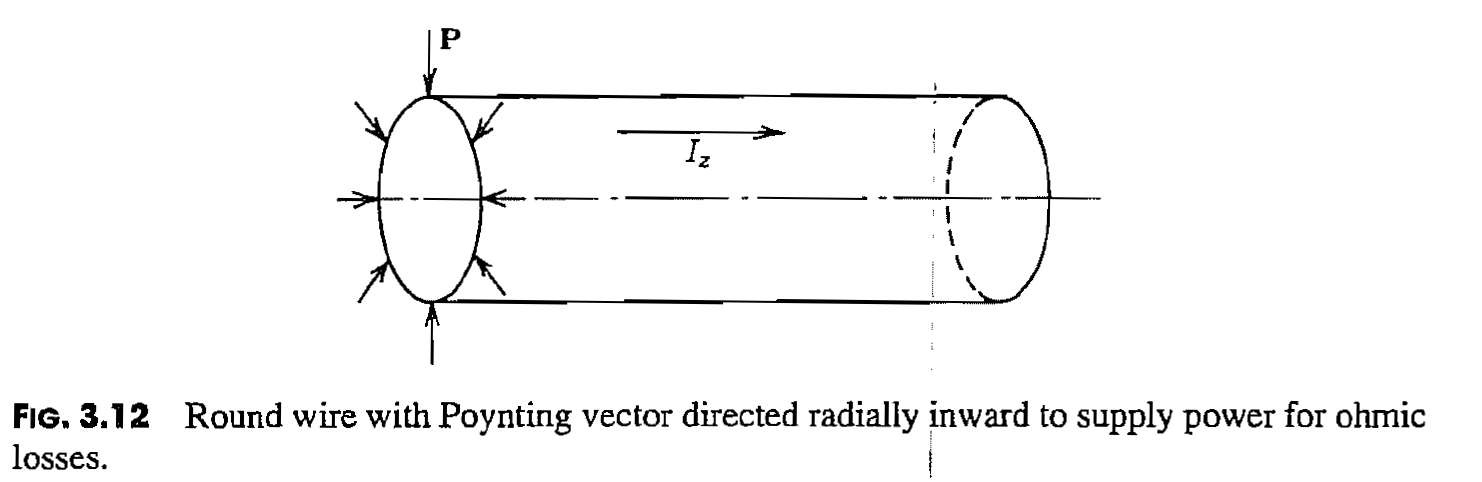
\includegraphics[scale = 0.5]{Ohmic loss.PNG} 
    
\end{figure}  

\footnote{FWC pag 142 } 

\newpage 

\section{Teorema di Poynting per un'onda piana}

\footnote{FWC - pag 143 | Example 3.12c Poynting flow in a plane wave} 

Data un'onda piana sinusoidale che varia in x e y con: 

{
    \Large
    \begin{equation}
        \begin{cases}
            E_x = E_o \cos(\omega t - \kappa z) \\
            H_y = \sqrt{\frac{\varepsilon}{\mu}} E_o \cos(\omega t - \kappa z)                         
        \end{cases}
    \end{equation}
}

che si propaga nella direzione z. \\

Dal teorema di Poynting: 
{
    \Large
    \begin{equation}
        \begin{split}
        \vec{P} 
        &= \vec{E} \times \vec{H} 
        \\ 
        &= \left|E_x\right| \left|H_y\right| \sin(\theta) 
        \end{split}
    \end{equation}
}

Essendo 
{
    \Large
    \begin{equation}
   \theta = 90 ^{\circ} 
   \rightarrow \sin(\theta) = 1     
    \end{equation}
} 

quindi: \\ 

{
    \Large
    \begin{equation}
        \begin{split}
            P_z 
            &= E_x H_y 
            \\
            &= \sqrt{\frac{\varepsilon}{\mu}} E_o ^{2} \cos^{2}(\omega t - \kappa z) 
            \\
            &= \frac{E_o ^{2}}{\eta } \cos^{2}(\omega t - \kappa z)        
        \end{split}
    \end{equation}
}

Utilizzando l'identità trigonometrica: 

{
    \Large
    \begin{equation}
    \sin^{2}(x) + \cos^{2}(x) = 1     
    \end{equation}
}

$P_z$ sarà:  

{
    \Large
    \begin{equation}
        \begin{split}
        P_z 
        &= 
        \sqrt{\frac{\varepsilon}{\mu}} E_o ^{2} [\frac{1}{2} + \frac{1}{2} \cos 2 (\omega t - \kappa z)] 
        \\ 
        &= \frac{E_o ^{2}}{\eta} [\frac{1}{2} + \frac{1}{2} \cos 2 (\omega t - \kappa z)]
        \end{split}
    \end{equation}
}

\begin{tcolorbox}
    Negli esercizi di esame, quando viene data la potenza dell'onda, il termine \\ $[\frac{1}{2} + \frac{1}{2} \cos 2 (\omega t - \kappa z)] = 0$, quindi \\ 

    $P_z = \frac{1}{2} \sqrt{\frac{\varepsilon}{\mu}} E_o ^{2} = \frac{E_o ^{2}}{2 \eta}$


\end{tcolorbox}

\newpage 

\section{Teorema di Poynting per i fasori} 

\footnote{FWC - pag 143 | 3.13 Poynting's theorem for phasors} 

Rispetto all'equazione di Maxwell in forma fasoriale, non possiamo sostituire $\jmath \omega$ a $\frac{\partial}{\partial t}$ per il 
Teorema di Poynting, quindi procediamo per step. \\ \\ 

Prendendo le equazione di Maxwell nella loro forma generale per i fasori: \\ 

{\Large \begin{equation}
    \begin{cases}
        \nabla \times \vec{E} = - \jmath \omega \vec{B} \\ 
        \nabla \times \vec{H} = \vec{J} + \jmath \omega \vec{D}
    \end{cases}
\end{equation}}

in cui, ricordiamo che: 

{
    \Large
    \begin{equation}
        \begin{cases}    
\vec{D} = \varepsilon \vec{E} 
\\
\vec{B} = \mu \vec{H}        
        \end{cases}
    \end{equation}
}

Consideriamo l'identità vettoriale: 

{
    \Large
    \begin{equation}
    \nabla \cdot (\vec{E}  \times \vec{H}^{*}) = \vec{H} ^{*} \cdot (\nabla \times \vec{E}) - \vec{E} \cdot (\nabla \times \vec{H} ^{*})        
    \end{equation}
}

dove l'asterisco denota il vettore complesso coniugato. 

\begin{tcolorbox}
    Dalla matematica, il vettore complesso coniugato è il vettore che ha lo stesso modulo del vettore originale, ma 
    verso opposto della parte immaginaria. \\ 

    Se vuoi approfondire: \\ \url{https://www.youmath.it/lezioni/analisi-matematica/numeri-complessi/3504-complesso-coniugato.html}


\end{tcolorbox}  

Applicando le equazioni di Maxwell in forma generale per i fasori, avremo che: 
{
    \Large
    \begin{equation}
    \nabla \cdot (\vec{E} \times \vec{H}^{*}) = \vec{H}^{*} \cdot (- \jmath \omega \vec{B}) - \vec{E} \cdot (\vec{J}^{*} - \jmath \omega \vec{D}^{*})      
    \end{equation}
}

Integrando entrambi i membri per un volume V e applicando il teorema della divergenza a entrambi i membri dell'equazione, avremo che: \\ 

{\Large \begin{equation}
    \begin{split}
        \int_V \nabla \cdot (\vec{E} \times \vec{H}^{*}) dV 
        &= \oint_S (\vec{E} \times \vec{H}^{*}) \cdot \vec{dS} 
        \\
        &= - \int_V [\vec{E} \cdot \vec{J}^{*} + \jmath \omega (\vec{H}^{*} \cdot \vec{B} - \vec{E} \cdot \vec{D}^{*})] dV       
    \end{split}
\end{equation}}

Questa è l'equazione generale del teorema Poynting in forma fasoriale. \\ \\ 

Sapendo che in un mezzo lineare isotropico 
{
    \Large
    \begin{equation}
    \vec{J} = \sigma \vec{E}         
    \end{equation}
}

e che $\sigma$, $\mu$ e $\varepsilon$ sono scalari, 
possiamo riscrivere il teorema di Poynting in forma fasoriale come: \\ 

{\Large \begin{equation}
    \oint_S (\vec{E} \times \vec{H}) \cdot dS = - \int_V \sigma \vec{E} \cdot \vec{E}^{*} dV - \jmath \omega \int_V [\mu \vec{H} \cdot \vec{H}^{*} - \varepsilon \vec{E} \cdot \vec{E}^{*}] dV
\end{equation}}

$- \int_v \sigma \vec{E} \cdot \vec{E}^{*} dV $ rappresenta il doppio della potenza media che si perde in un conduttore 
di corrente, quindi la potenza media è: 

{\Large \begin{equation}
    P_{av} = \frac{1}{2} \Re(\vec{E} \times \vec{H}^{*})
\end{equation}}


$P_{av}$ si misura in $[\frac{W}{m^2}]$ \\ (si legge Watt per metro quadro)  \\ \\ 

Per un mezzo lineare isotropico:

{
    \Large
    \begin{equation}
    - \jmath \omega \int_V [\mu \vec{H} \cdot \vec{H}^{*} - \varepsilon \vec{E} \cdot \vec{E}^{*}] dV = -\jmath \omega \int_V \frac{1}{2} [\frac{1}{2} \varepsilon \left|E\right|^{2} - \frac{1}{2} \mu \left|H\right|^{2} ] dV    
    \end{equation}
}

Allora: 
{\Large \begin{equation}
    \Im\oint_S (\vec{E} \times \vec{H}^{*}) \cdot \vec{dS} = 4\omega (U_{Eav} - U_{Hav})
\end{equation}}

dove $U_{Eav}$ e $U_{Hav}$ sono rispettivamente l'energia immagazzinata di campo elettrico e di campo magnetico. \\ \\ 

Quindi, la parte immmaginaria del teorema di Poynting può essere vista come la potenza reattiva, cioè la potenza opposta 
alla direzione di propagazione dell'onda. 

\newpage 

\section{Potenza media in un'onda piana uniforme} 

\footnote{FWC - pag 145 | Example 3.13 Average power in uniform plane waves} 

Considerando le onde piane scritte in forma fasoriale: 

{\Large \begin{equation}
    \begin{cases}
        E_x = C_1 e^{-\jmath \kappa z} + C_2 e^{\jmath \kappa z} \\ 
        H_y = \sqrt{\frac{\varepsilon}{\mu}} [C_1 e^{-\jmath \kappa z} + C_2 e^{\jmath \kappa z}] 
    \end{cases}
\end{equation}}

\begin{tcolorbox}
    L'onda qui indicato è polarizzata linearmente per $E_x$. \\ 
    La polazizzione è un argomento che andremo ad affrontare in un capitolo futuro. 
\end{tcolorbox}


Il vettore Poynting in forma complessa è: 

{\Large \begin{equation}
    \vec{E} \times \vec{H} = \sqrt{\frac{\varepsilon}{\mu}} [C_1 e^{-\jmath \kappa z} + C_2 e^{\jmath \kappa z}] [C_1^{*} e^{-\jmath \kappa z} + C_2^{*} e^{\jmath \kappa z}] \hat{z}
\end{equation}}

Quindi, la potenza media lungo la direzione z è: 

{\Large \begin{equation}
    P_{av} = \frac{1}{2} \sqrt{\frac{\varepsilon}{\mu}} [C_1 C_1^{*} - C_2 C_2^{*}]
\end{equation}}

$P_{av}$ esprime che la potenza media lungo z è uguale alla potenza dell'onda lungo z sottratto alla potenza 
dell'onda lungo -z. \\ \\ 

\newpage 

 
\include{4 - Continuità dei campi} 
\chapter{Onde piane} 

\begin{figure}[h]
    \centering
    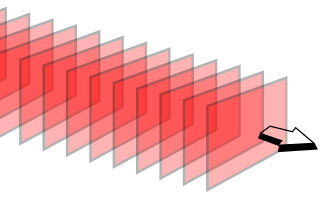
\includegraphics{Plane_wave_wavefronts_3D.png}
    
\end{figure} 

\newpage 

\section{Onde piane - Equazioni e coefficienti}
\footnote{FWC - pag 275 | 6.2 Uniform plane waves in a perfect dielectric} 

Ricordando le leggi di Maxwell, possiamo applicarle alle onde piane: 

{\Large \begin{equation}
    \begin{cases}
        \nabla \cdot \vec{E} = 0 \\ 
        \nabla \cdot \vec{H} = 0 \\ 
        \nabla \times \vec{E} = -\mu \frac{\partial \vec{H}}{\partial t} \\ 
        \nabla \times \vec{H} = \varepsilon \frac{\partial \vec{E}}{\partial t}
    \end{cases}
\end{equation}} 

In fisica matematica, un'onda piana è un'onda a frequenza costante i cui fronti d'onda sono infiniti piani paralleli perpendicolari alla direzione di propagazione, e la cui distanza picco-picco è costante. \\ 

L'onda piana rappresenta un'astrazione matematica che non corrisponde ad alcun fenomeno fisico equivalente in senso stretto, poiché a partire da una descrizione analitica esatta si ottiene un'onda che per essere generata necessita di una sorgente di lunghezza infinita. \\ \\
L'onda piana è tuttavia utilizzata per approssimare il caso in cui la sorgente dell'onda è posta a distanza infinita dal punto di osservazione del fronte d'onda considerato, che viene quindi assunto localmente piano. \\ \\ 
Una caratteristica che la differenzia da altri tipi di propagazione ondosa, come l'onda sferica (tridimensionale) o quella circolare (in due dimensioni), è l'assenza di attenuazione isotropica nello spazio, in virtù della direzionalità dell'emissione e della propagazione di energia associata all'onda. L'unica attenuazione che si verifica è dovuta all'eventuale assorbimento da parte del materiale del mezzo di propagazione attraversato. 

\footnote{Wikipedia - Onde piane} \\

Possiamo scrivere l'onda piana come un'onda che si propaga 
lungo l'asse z (asse scelto da noi come quello di propagazione, l'onda piana può propagarsi anche negli altri due assi) 
come: \\ 

{\Large \begin{equation}
    E_x (z, t) = f_1 (t-\frac{z}{v}) + f_2 (t-\frac{z}{v}) 
\end{equation}}

dove: 
{
    \Large
    \begin{equation}
        v = \frac{1}{\sqrt{\mu \varepsilon}} 
    \end{equation}
}

v è la velocità della luce nel mezzo. \\ \\ 

Possiamo scrivere: 

{\Large \begin{equation}
    E_x ^{+} = f_1 (t - \frac{z}{v})
\end{equation}}

l'onda che si propaga lungo l'asse z. 

{\Large \begin{equation}
    E_x ^{-} = f_2 (t + \frac{z}{v})
\end{equation}} 

l'onda che si propaga lungo l'asse -z. \\ \\ 


Con lo stesso principio, e sempre grazie alle leggi di Maxwell, possiamo scrivere: 

{\Large \begin{equation}
    \begin{split}
        H_y 
        &= H_y ^{+} H_y ^{-} 
        \\
        &= \frac{E_x ^{+}}{\eta} - \frac{E_x ^{-}}{\eta} 
    \end{split}
\end{equation}}

dove: \\ 

{\Large \begin{equation}
    \eta = \sqrt{\frac{\mu}{\varepsilon}}
\end{equation}}

$\eta$ si può ricavare anche come: 

{\Large \begin{equation}
    \eta = \frac{E_x}{H_y}    
\end{equation}} 

Grazie a questo rapporto, $\eta$ prende il nome di Impedenza intrinsica nel mezzo. 

Nel vuoto: 
{\Large \begin{equation}
    \eta_o = \sqrt{\frac{\mu_o}{\varepsilon_o}} = 376,73 [\Omega] \approx 120 \pi [\Omega]
\end{equation}}

\begin{tcolorbox}
$\Omega$ (lettera greca Omega, ma in questo caso rappresente l'unità di misura Ohm)  è la stessa 
unità di misura usata nei circuiti elettronici. 
    
\end{tcolorbox}

Quello che abbiamo visto con $E_x$ e $H_y$, è possibile anche con $E_y$ e $H_x$. 

{\Large \begin{equation}
    \begin{cases}
        E_y = f_3 (t-\frac{z}{v}) + f_4 (t+\frac{z}{v}) = E_y ^{+} + E_y ^{-} \\ \\
        H_x = - \frac{E_y ^{+}}{\eta} + \frac{E_y ^{-}}{\eta}     
    \end{cases}
\end{equation}} 

Quindi possiamo scrivere: 

{\Large \begin{equation}
    \begin{cases}
        \frac{E_x ^{+}}{H_y ^{+}} = -\frac{E_y ^{+}}{H_x ^{+}} = \eta \\ 
        \frac{E_x ^{-}}{H_y ^{-}} = -\frac{E_y ^{-}}{H_x ^{-}} = - \eta
    \end{cases}
\end{equation}} 

Da queste relazioni possiamo scrivere, se E è perpenicolare a H: 

{\Large \begin{equation}
    E = \eta H
\end{equation}} 




Dal Teorema di Poynting, possiamo scrivere la potenza dell'onda lungo l'asse z come: 

{\Large \begin{equation}
    \begin{split}
        P_z ^{+} 
        &= E_x ^{+} H_y ^{+} - E_y ^{+} H_x ^{+} 
        \\
        &= \frac{1}{\eta} (E_x ^{+^{2}} + E_y ^{+^{2}}) 
    \end{split}
\end{equation}}

\begin{figure}[h]
    \centering
    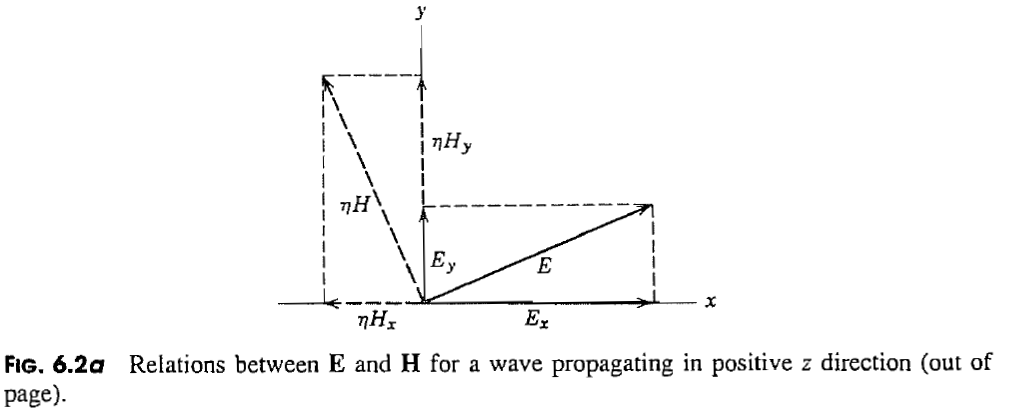
\includegraphics[scale = 0.6]{E and H in a plane wave.PNG}
\end{figure} 

\footnote{FWC - pag 277} 

\newpage 

\section{Onde piane in forma fasoriale} 

\footnote{FWC - pag 275 | 6.2 Uniform plane waves in a perfect dielectric} 

Estendendo l'analisi in forma fasoriale: 

{\Large \begin{equation}
    \begin{cases}
        E_x (z) = E_1 e^{-\jmath \kappa z} + E_2 e^{\jmath \kappa z} \\ 
        \eta H_y (z) = E_1 e^{-\jmath \kappa z} - E_2 e^{\jmath \kappa z} \\ \\ 

        E_y (z) = E_3 e^{-\jmath \kappa z} + E_4 e^{\jmath \kappa z} \\ 
        \eta H_x (z) = - E_3 e^{-\jmath \kappa z} + E_4 e^{\jmath \kappa z}

    \end{cases}
\end{equation}} 


dove: 

{\Large \begin{equation}
    \kappa = \frac{\omega}{v} = v \sqrt{\mu \varepsilon}
\end{equation}}

$\kappa$ è chiamata numero d'onda (in inglese wave number). \\ 
$\kappa$ è la fase dell'onda, in cui nelle onde piane è costante. \\ 

La lunghezza dell'onda $\lambda$ (si legge lambda) è il valore di z in cui la fase cambia di $2 \pi$. 

{\Large \begin{equation}
    \kappa \lambda = 2 \pi 
    \Rightarrow \kappa = \frac{2 \pi}{\lambda}
\end{equation}} 


{\Large \begin{equation}
    \lambda = \frac{2 \pi}{\kappa} = \frac{2 \pi}{\omega \sqrt{\mu \varepsilon}} = \frac{v}{f} 
\end{equation}}

Per calcolare la lunghezza d'onda nel vuoto, possiamo sostituire a v la velocità della luce, indicata anche come c. \\ 

In ottica, si sceglie di indicare $\lambda$ come n, dove n prende il nome di indice refrattivo (in inglese refractive index). 

{\Large \begin{equation}
    n = \frac{c}{v} = \sqrt{\frac{\mu \varepsilon}{\mu_o \varepsilon_o}}
\end{equation}}

Per molti materiali in ottica, e anche per materiali non magnetici, $\mu = \mu_o$

\newpage

\section{Polarizzazione delle onde piane} 
\footnote{FWC - pag 280 | 6.3 Polarization of plane waves} 

Se diverse onde piane hanno la stessa direzione di propagazione, 
possiamo sovrapporre queste onde per un mezzo lineare. \\ 

L'orientazione dei campi vettoriali, sia della singola onda che delle altre, è descritta dalla polarizzazione delle onde 
(in questo inserto parleremo solo di onde della stessa frequenza). \\ 

Prendiamo solo un'onda lungo l'asse z, usando la rappresentazione fasoriale e assumiamo sia x e y componenti del campo elettrico. \\ \\ 
L'espressione generale per quest'onda è la seguente: 

{\Large \begin{equation}
    \vec{E} = (\hat{x} E_1 + \hat{y} E_2 e^{\jmath \psi } e^{-\jmath \kappa z})
\end{equation}}

dove $E_1$ e $E_2$ sono reali e $\psi$ (si legge psi) è l'angolo tra le componenti x e y. \\ 

Il corrispondente campo magnetico è: 

{\Large \begin{equation}
    \vec{H} = \frac{1}{\eta} (-\hat{x} E_2 e^{\jmath \psi} + \hat{y}E_1) e^{-\jmath \kappa z}
\end{equation}}

Le onde possono essere anche non polarizzate. \\ 

Ci sono diverse classi di polarizzazione che dipendono dalla fase e dalle ampiezze di $E_1$ e $E_2$. \\ \\ 

\newpage 

\subsection{Polarizzazione lineare o planare}

\begin{figure}[h]
    \centering
    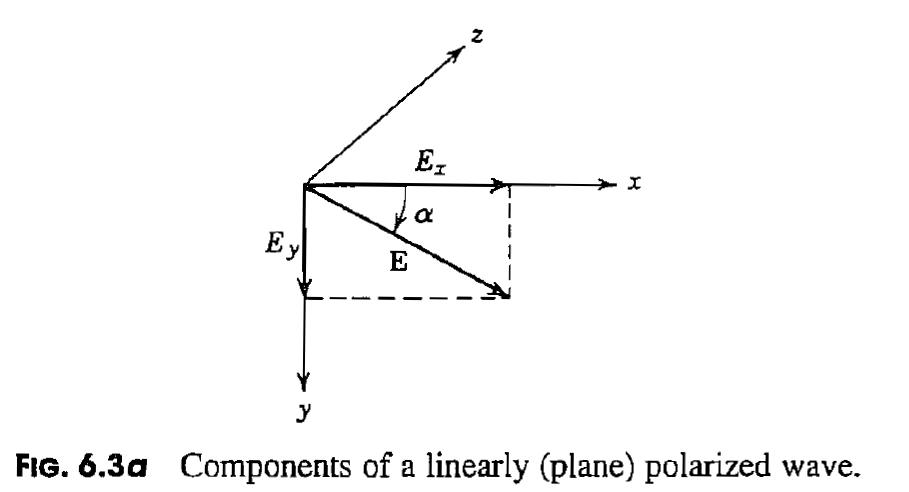
\includegraphics[scale = 0.8]{Linearly polarized wave.PNG}
    
\end{figure}

\footnote{FWC - pag 280}

Se i due campi sono in fase, cioè $\psi = 0$, ogni piano in z sarà definito da un angolo rispetto all'asse x chiamato $\alpha$ (si legge alfa) come: 

{\Large \begin{equation}
    \alpha = \arctan \frac{E_y}{E_x} = \arctan \frac{E_2}{E_1}
\end{equation}}

\begin{tcolorbox}
    $\arctan$ è l'inverso della funzione tangente. \\ $\arctan$ = $\tan ^{-1}$ 
\end{tcolorbox}

Questo angolo è reale, quindi è lo stesso per tutti i valori di z e t. \\ 

Siccome $\vec{E}$ mantiene la sua direzione nello spazio, questa polarizzazione è chiamata lineare, o polarizzazione planare perchè il vettore 
del campo elettrico definisce un piano che si propaga lungo la direzione z. \\ 

\newpage 

\subsection{Polarizzazione circolare} 

\begin{figure}[h]
    \centering
    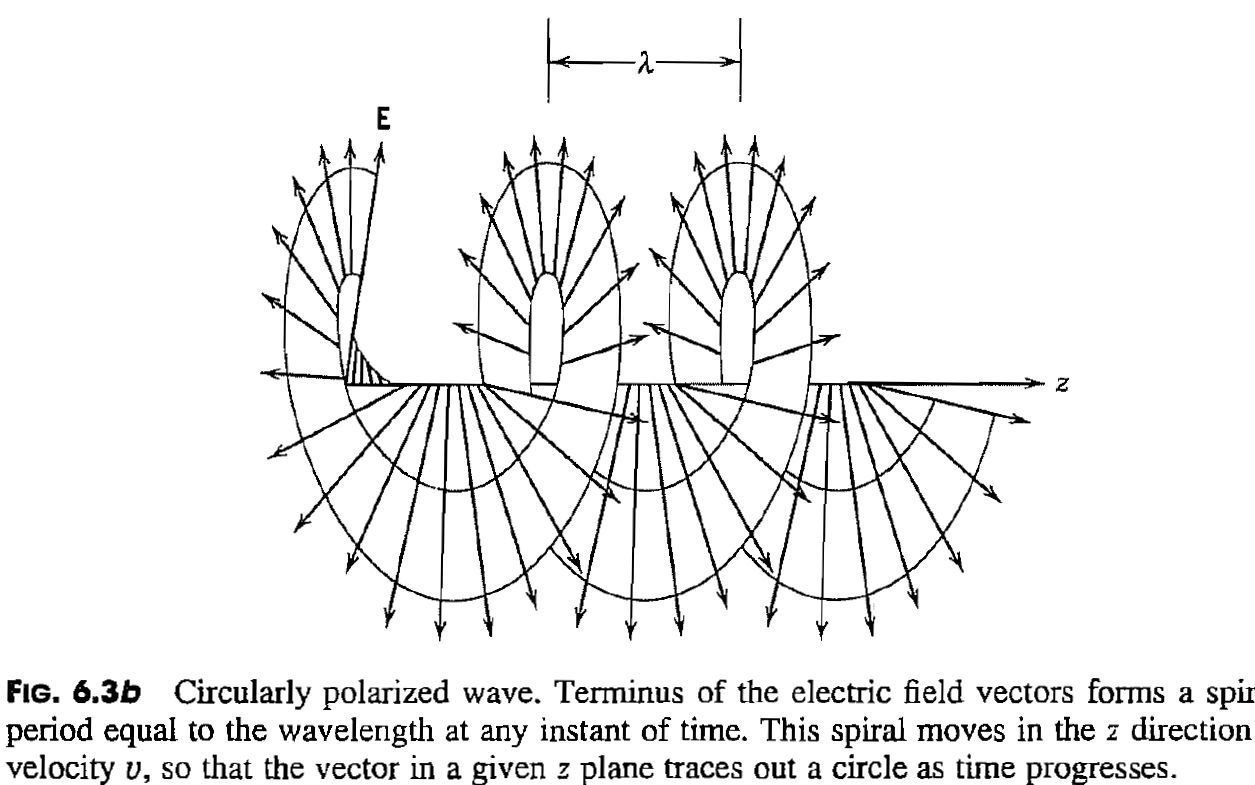
\includegraphics[scale = 0.5]{Circularly polarized wave.PNG}
    
\end{figure}

\footnote{FWC - pag 281}

Nella polarizzazione circolare: 

{\Large \begin{equation}
    \begin{cases}
        E_1 = E_2 \\ 
        \psi = \pm  \frac{\pi}{2}   
    \end{cases}
\end{equation}}

Quindi, con le dovute sostituzioni: 

{\Large \begin{equation}
    \begin{split}
    \vec{E} 
    &= (\hat{x} E_1 + \hat{y} E_2 e^{\jmath \psi } e^{-\jmath \kappa z}) 
    \\
    &\Rightarrow  \vec{E} = (\hat{x} + \pm \jmath \hat{y}) E_1 e^{- \jmath \kappa z}
    \end{split}
\end{equation}}

L'ampiezza di $\vec{E}$ è $\sqrt{2} E_1$ e il vettore $\vec{E}$ è un vettore che si muove in modo circolare. \\ 

La forma instantanea di un'onda polarizzata circolarmente: 

{\Large \begin{equation}
    \begin{split}
        \vec{E} (z, t) &= \Re [(\hat{x} + \pm \jmath \hat{y}) E_1 e^{- \jmath \kappa z} ]  \\
        &= E_1 [\hat{x} \cos(\omega t - \kappa z) \mp \hat{y} \sin(\omega t -\kappa z) ]    
    \end{split}
\end{equation}}

La somma del quadrato delle forme instantanee di $E_x$ e $E_y$ da: 

{\Large \begin{equation}
    \begin{split}
        E_x ^{2} (z, t) + E_y ^{2} (z, t) 
        &= E_1 ^{2} [\cos^{2}(\omega t - \kappa z) + \sin^{2}(\omega t - \kappa z)] 
        \\
        &= E_1 ^{2}
    \end{split}
\end{equation}}

Equazione che definisce un cerchio. \\ 

L'angolo instantaneo $\alpha$ rispetto all'asse x è: 

{\Large \begin{equation}
    \begin{split}
        \alpha 
        &= \arctan \frac{E_y(z, t)}{E_x(z, t)} 
        \\
        &= \arctan (\frac{\sin(\omega t - \kappa z)}{\cos(\omega t - \kappa z)}) 
        \\
        &= \mp (\omega t - \kappa z)
    \end{split}
\end{equation}}


Dato un piano z, il vettore ruota con una velocità costante angolare di $\alpha = \mp \omega t$. \\ 

La propagazione dell'onda è di tipo epicicloidale (come il movimento di un cavatappi) lungo la direzione z con una velocità v. \\ 

Da notare che (per z = 0)
{\Large \begin{equation}
    \begin{cases}
     \psi = + \frac{\pi}{2} \Rightarrow \alpha = -\omega t \\ 
     \psi = - \frac{\pi}{2} \Rightarrow \alpha = \omega t 
    \end{cases}
\end{equation}}

Nel primo caso, l'onda si muove in senso anti-orario, nel secondo caso in senso orario. \\ 

Ricordando che se $E_1 = E_2$ e $\psi = \pm \frac{\pi}{2}$, il relativo campo magnetico di un'onda polarizzata in modo circolare è: 

{\Large \begin{equation}
    \vec{H} = \frac{E_1}{\eta} (\mp \jmath \hat{x} + \hat{y}) e^{- \jmath \kappa z}
\end{equation}}


\newpage 

\subsection{Polarizzazione elittica} 


\begin{figure}[h]
    \centering
    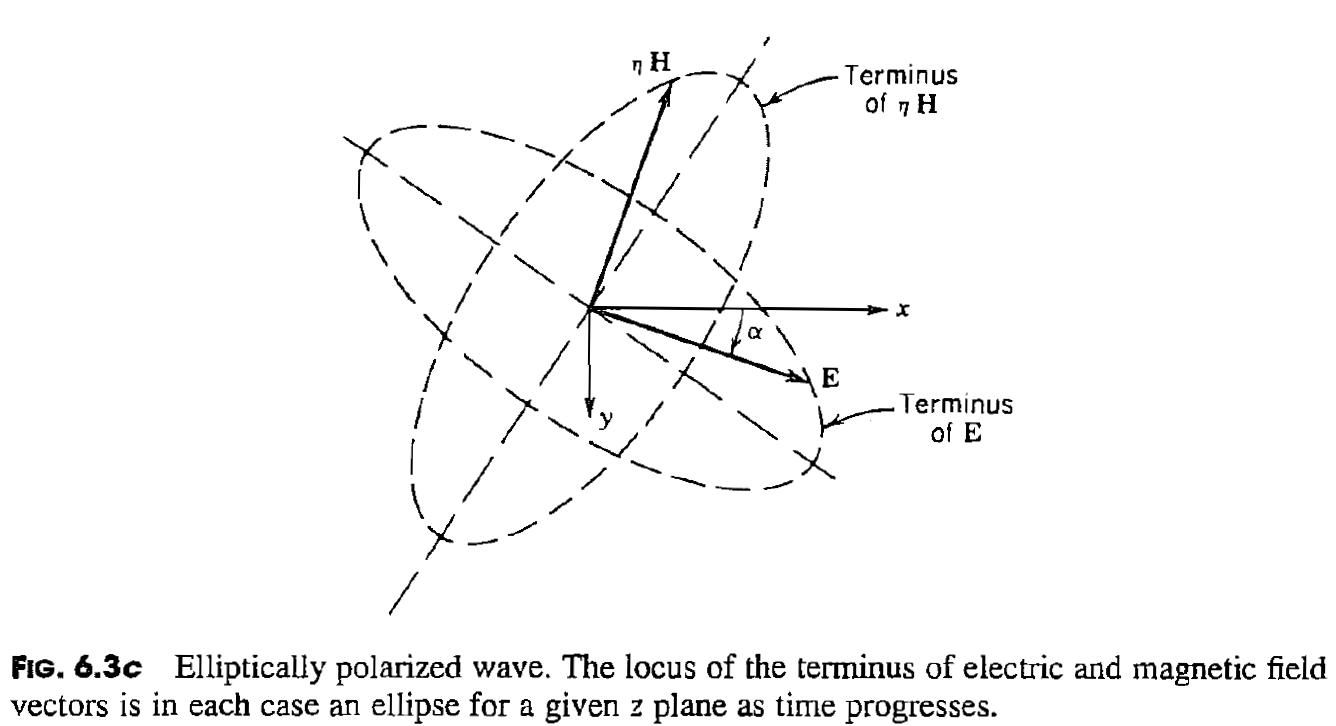
\includegraphics[scale = 0.5]{Elliptically polarized wave.PNG}
    
\end{figure}

\footnote{FWC - pag 282}


Per il caso generale, con $E_1 \neq E_2$ o $E_1 = E_2$, ma $\psi$ è diverso da 0 o da $\mp \frac{\pi}{2}$ . \\ \\
Quindi, per il caso generale, l'onda descrive una traiettoria di un elisse, quindi il nome di questa polarizzazione è detta elittica. \\ 

La forma instantanea di questo tipo d'onda è: 

{\Large \begin{equation}
    \begin{split}
        \vec{E} (z, t) &= \Re[(\hat{x} E_1 + \hat{y} E_2 e^{\jmath \psi}) e^{\jmath \omega t} e^{-\jmath \kappa z}] 
        \\ &= 
    \hat{x} E_1 \cos(\omega t - \kappa z) + \hat{y} E_2 \cos(\omega t - \kappa z + \psi) 
    \end{split}
\end{equation}}


Per un qualsiasi piano, poniamo z=0, 

{\Large \begin{equation}
    \begin{cases}
        E_x (z, t) = E_1 \cos(\omega t) \\ 
        E_y (z, t) = E_2 \cos(\omega t + \psi)     
    \end{cases}
\end{equation}}

 
\chapter{Onde piane TEM tra due materiali} 
\begin{figure}[h]
    \centering
    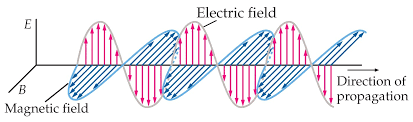
\includegraphics{TEM plane waves.png}
    
\end{figure}    

\newpage

\section{Riflessione e trasmissione delle onde piane con incidenza normale (TEM)}

\footnote{FCE - Pag 311 | 8.1.1 Interfaccia tra mezzi senza perdite \\ 
FAE - Pag 339 | 8.1.1 Boundary between lossless media} 

Per onde TEM (Transverse Electro-Magnetic Waves) si intendono onde in cui campi 
elettrico e magnetico hanno direzione ortogonale rispetto a quella del vettore di propagazione. 

\begin{figure}[h]
    \centering
    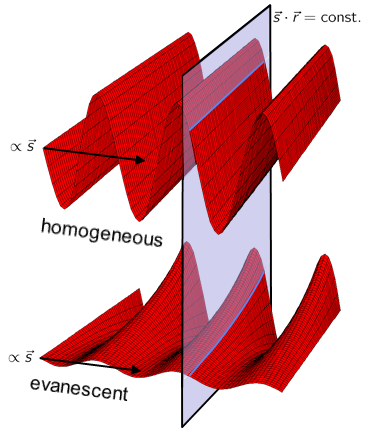
\includegraphics{plane_waves_hom_evan.png}    
\end{figure}    
\footnote{\url{https://www.pvlighthouse.com.au/it/cms/lectures/altermatt/optics/planar-transversal-electromagnetic-waves}} 


Consideriamo questo piano: 

\begin{figure}[h]
    \centering
    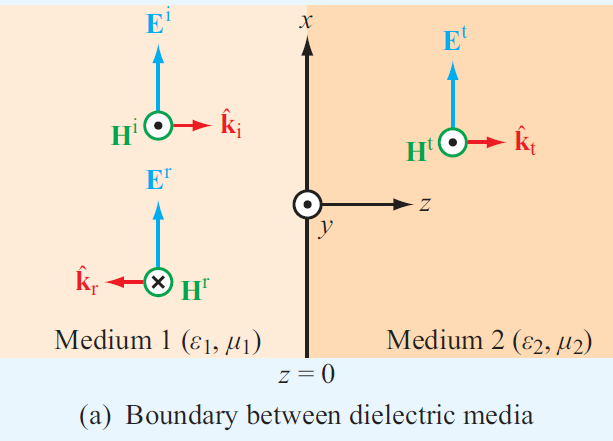
\includegraphics[scale = 0.6]{TEM EM waves.PNG}    
\end{figure}    
\footnote{FAE - pag 340}

in cui il tondino con il punto indica che l'asse esce dal foglio. \\

Possiamo rappresentare, dal punto di vista grafico, anche in questa maniera: \\ \\ 

\begin{figure}[h]
    \centering
    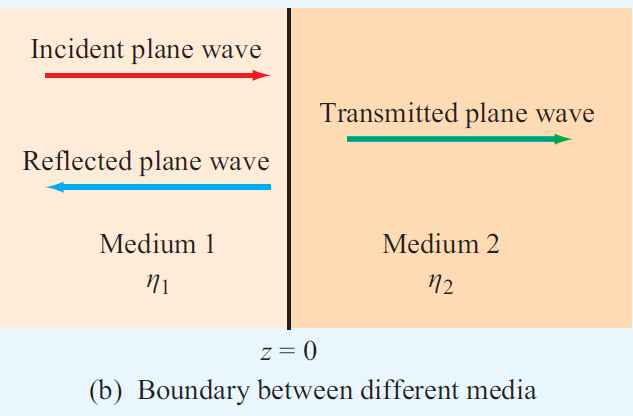
\includegraphics[scale = 0.6]{EM between two mediums.PNG}    
\end{figure}

\footnote{FAE - pag 339}


Esplicitiamo le equazioni delle onde piane: \\ \\ 

\textbf{Onda incidente:} 
{\Large \begin{equation}
    \begin{cases}
        \vec{E^{i}}(z) = \hat{x} E_o ^{i} e^{-\jmath \kappa_1 z} \\ 
        \vec{H^{i}}(z) = \hat{y} \frac{E_o ^{i}}{\eta_1} e^{-\jmath \kappa_1 z}  
    \end{cases}
\end{equation}}


\textbf{Onda riflessa:} 
{\Large \begin{equation}
    \begin{cases}
        \vec{E^{r}}(z) = \hat{x} E_o ^{r} e^{\jmath \kappa_1 z} \\ 
        \vec{H^{r}}(z) = -\hat{y} \frac{E_o ^{r}}{\eta_1} e^{\jmath \kappa_1 z}  
    \end{cases}
\end{equation}}

\textbf{Onda trasmessa:} 
{\Large \begin{equation}
    \begin{cases}
        \vec{E^{t}}(z) = \hat{x} E_o ^{t} e^{-\jmath \kappa_2 z} \\ 
        \vec{H^{t}}(z) = \hat{y} \frac{E_o ^{t}}{\eta_2} e^{-\jmath \kappa_2 z}  
    \end{cases}
\end{equation}}

dove: 

{\Large \begin{equation}
    \begin{cases}
        \kappa_1 = \omega \sqrt{\mu_1 \varepsilon_1} \\ 
        \kappa_2 = \omega \sqrt{\mu_2 \varepsilon_2} \\ 
        \eta_1 = \sqrt{\frac{\mu_1}{\varepsilon_1}} \\ 
        \eta_2 = \sqrt{\frac{\mu_2}{\varepsilon_2}} \\ 
    \end{cases}
\end{equation}}

$E_o ^{i}$, $E_o ^{r}$,  $E_o ^{t}$ sono le ampiezze delle onde, rispettivamente, dell'onda incidente, riflessa e trasmessa. \\ 

I numeri dei coefficienti (1 e 2) indicano in quale piano si trovano le onde. \\ \\ 

Dal capitolo 4 sulla continuità dei campi, sappiamo che il componente tangente di $\vec{E}$ è sempre continuo in un'interfaccia tra due mezzi adiacenti. \\ 
Inoltre, in assenza di corrente sull'interfaccia, anche il componente tangenziale di $\vec{H}$ è continuo tra due mezzi adiacenti. \\ \\ 

Quindi nel mezzo 1, l'onda sarà: \\ 

{\Large \begin{equation}
    \begin{cases}
        \vec{E_1 }(z) = \vec{E^{i}} (z) + \vec{E^{r} }(z) = \hat{x} (E_o ^{i} e^{-\jmath \kappa_1 z} + E_o ^{r} e^{\jmath \kappa_1 z} ) \\ 
        \vec{H_1} (z) = \vec{H^{i}} (z) + \vec{H^{r}} (z) = \hat{y} \frac{1}{\eta_1} (E_o ^{i} e^{-\jmath \kappa_1 z} + E_o ^{r} e^{\jmath \kappa_1 z} )    
    \end{cases}
\end{equation}}

Per adesso, nel mezzo 2 è solo presente l'onda trasmessa, quindi: 

{\Large \begin{equation}
    \begin{cases}
        \vec{E_2} (z) = \vec{E^{t}} (z) = \hat{x} E_o ^{t} e^{-\jmath \kappa_2 z} \\ 
        \vec{H_2} (z) = \vec{H^{t}} (z) = \hat{y} \frac{E_o ^{t}}{\eta_2} e^{-\jmath \kappa_2 z}    
    \end{cases}
\end{equation}}

Ponendoci all'interfaccia $z = 0$, i componenti tangenziali dei campi elettrico e magnetico sono continui. \\ 

In formule: 

{\Large \begin{equation}
    \begin{cases}
        \vec{E_1} (z = 0) = \vec{E_2} (z= 0) \Rightarrow E_o ^{i} + E_o ^{r} = E_o ^{t} \\ 
        \vec{H_1} (z = 0) = \vec{H_2} (z= 0) \Rightarrow \frac{E_o ^{i}}{\eta_1} - \frac{E_o ^{r}}{\eta_1} = \frac{E_o ^{t}}{\eta_2} 
    \end{cases}
\end{equation}}

Risolvendo il sistema per ricavare $E_o ^{r}$ in funzione di $E_o ^{i}$ (quindi poniamo $E_o ^{i}$ come variabile indipipenente), 
avremo che: 

{\Large \begin{equation}
    \begin{split}
        E_o ^{r} 
        &= \frac{\eta_2 - \eta_1}{\eta_2 + \eta_1} E_o ^{i} 
        \\
        &= \Gamma E_o ^{i}   
    \end{split}
\end{equation}}

\begin{tcolorbox}
    $\Gamma$ si legge gamma 
\end{tcolorbox}

Risolvendo il sistema per ricavare $E_o ^{t}$ in funzione di $E_o ^{i}$, avremo che: 

{\Large \begin{equation}
    \begin{split}
        E_o ^{t} 
        &= \frac{2 \eta_2 }{\eta_2 + \eta_1} E_o ^{i} 
        \\
        &=  \tau E_o ^{i}   
    \end{split}
\end{equation}}

dove: 

{\Large \begin{equation}
    \Gamma = \frac{E_o ^{r}}{E_o ^{i}} = \frac{\eta_2 - \eta_1}{\eta_2 + \eta_1}
\end{equation}}

$\Gamma$ prende il nome di coefficiente di riflessione. 

{\Large \begin{equation}
    \tau = \frac{E_o ^{t}}{E_o ^{i}} = \frac{2 \eta_2}{\eta_2 + \eta_1} 
\end{equation}}

$\tau$ prende il nome di coefficiente di trasmissione. \\ 

Se $\eta_1$ e $\eta_2$ sono reali, anche $\Gamma$ e $\tau$ lo sono. \\ \\  

$\tau$ si può esprimere come: 

{\Large \begin{equation}
    \tau = 1 + \Gamma    
\end{equation}}

Si può esprimere $\eta_1$ e $\eta_2$ come: 

{\Large \begin{equation}
    \begin{cases}
        \eta_1 = \frac{\eta_o}{\sqrt{\varepsilon_{r1}}} \\ 
        \eta_2 = \frac{\eta_o}{\sqrt{\varepsilon_{r2}}} 
    \end{cases}
\end{equation}}

dove: 

{\Large \begin{equation}
    \eta_o = \sqrt{\frac{\mu_o}{\varepsilon_o}} \approx 377 [\Omega] 
\end{equation}}

$\eta_o$ prende il nome di impedenza intrinsica nello spazio libero. \\ \\ 

$\Gamma$ si può scrivere nei materiali non magnetici anche come: \\

{\Large \begin{equation}
    \Gamma = \frac{\sqrt{\varepsilon_{r1}} - \sqrt{\varepsilon_{r2}}}{ \sqrt{\varepsilon_{r1}} + \sqrt{\varepsilon_{r2}}}
\end{equation}}

\newpage 

\section{Flusso di potenza nei mezzi senza perdite} 

\footnote{FCE - pag 315 | 8.1.3 Flusso di potenza nei mezzi senza perdite \\ 
FAE - pag 341 | 8.1.1 Power Flow in Lossless media}

Utilizzando il teorema di Poynting, la densità media netta che flusice nel mezzo 1 è: 

{\Large \begin{equation}
    \begin{split}
        \vec{S_{av_1}} &= \frac{1}{2} \Re [\vec{E_1}(z) \times \vec{H_1} ^ {*} (z) ] 
        \\
        &= \frac{1}{2} \Re [\hat{x} E_o ^{i} (e^{-\jmath \kappa_1 z} + \Gamma e^{\jmath \kappa_1 z}) \times  \hat{y} \frac{E_o ^{i^*}}{\eta_1} (e^{\jmath \kappa_1 z} - \Gamma e^{-\jmath \kappa_1 z})]\\ 
        &= \hat{z} \frac{\left|E_o ^{i}\right| ^{2}}{2 \eta_1} (1 - \left|\Gamma\right| ^{2})    
    \end{split}
\end{equation}} 

$\vec{S_{av_1}}$ lo si può esprimere anche come: 

{\Large \begin{equation}
    \vec{S_{av_1}} = \vec{S_{av} ^{i}} + \vec{S_{av} ^{r}}    
\end{equation}} 

dove: 

{\Large \begin{equation}
    \begin{cases}
        \vec{S_{av} ^{i}} = \hat{z} \frac{\left|E_o ^{i}\right|}{2 \eta_1} \\ 
        \vec{S_{av} ^{r}} = - \hat{z}  \left|\Gamma\right|^{2} \frac{\left|E_o ^{i}\right|}{2 \eta_1} = - \left|\Gamma\right|^{2} \vec{S_{av} ^{i}}\\ 
    \end{cases}
\end{equation}}

$\vec{S_{av} ^{i}}$ è la densità di energia media dell'onda incidente nel mezzo 1, 
mentre $\vec{S_{av} ^{r}}$ è la densità di energia media dell'onda riflessa nel mezzo 1. \\ \\ 

La densità di potenza media nel mezzo 2 è: 

{\Large \begin{equation}
    \begin{split}
    \vec{S_{av_2}} &= \frac{1}{2} \Re [\vec{E_2}(z) \times \vec{H_2} ^ {*} (z) ] \\
    &= \frac{1}{2} \Re [\hat{x} \tau E_o ^{i} e^{-\jmath \kappa_2 z} \times  \hat{y} \tau^{*} \frac{E_o ^{i^*}}{\eta_2} e^{\jmath \kappa_2 z}] \\ 
    &= \hat{z} \left|\tau\right| ^{2} \frac{\left|E_o ^{i}\right| ^{2}}{2 \eta_2}
    \end{split}
\end{equation}}

Nei mezzi senza perdite: 
{\Large \begin{equation}
    \frac{\tau ^{2}}{\eta_2} = \frac{1 - \Gamma ^{2}}{\eta_1}
\end{equation}} 

da cui: 

{\Large \begin{equation}
    \vec{S_{av_1}} = \vec{S_{av_2}} 
\end{equation}}

\newpage


\section{Leggi di Snell} 

\footnote{FCE - pag 322 | 8.2 Legge di Snell \\ 
FAE - pag 349 | 8.2 Snell's Laws} 

\begin{figure}[h]
    \centering
    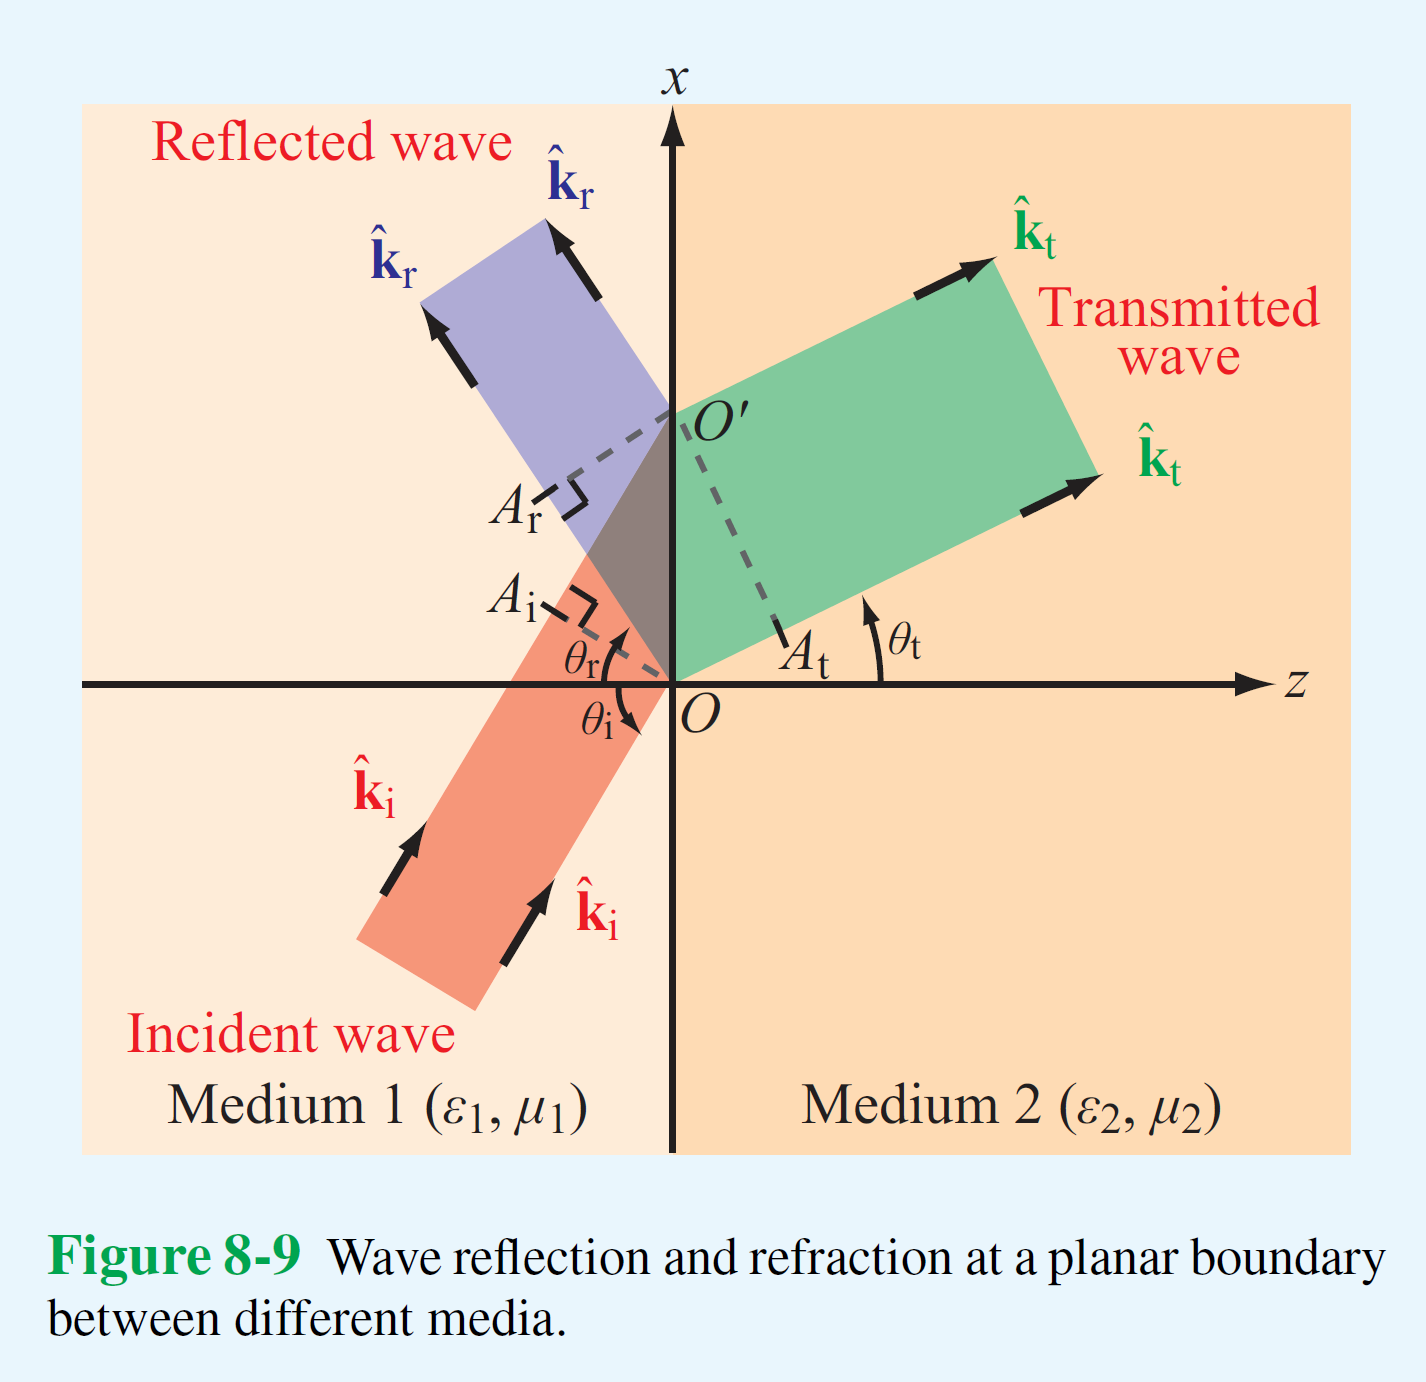
\includegraphics[scale = 0.8]{Wave reflectaion in a boundary.PNG}
    
\end{figure} 

Considerando un'interfaccia a $z=0$ per due mezzi diversi, mezzo 1 con $\varepsilon_1$, $\mu_1$ e 
mezzo 2 con $\varepsilon_2$, $\mu_2$ e: \\ 

$\theta_i$ angolo di incidenza \\ 
$\theta_r$ angolo di riflessione \\ 
$\theta_t$ angolo di trasmissione (o rifrazione) \\ \\ 

Indicando con $u_{p_1}$ e $u_{p_2}$ le velocità dell'onda nei mezzi 1 e 2: 

{\Large \begin{equation}
    \begin{cases}
        u_{p_1} = \frac{1}{\sqrt{\mu_1 \varepsilon_1}}\\ 
        u_{p_2} = \frac{1}{\sqrt{\mu_2 \varepsilon_2}} 
    \end{cases}
\end{equation}} 

Possiamo esprimere le leggi di Snell: 

{\Large \begin{equation}
    \begin{cases}
        \theta_i = \theta_r \\ 
        \frac{\sin(\theta_t)}{\sin(\theta_i)} = \frac{u_{p_2}}{u_{p_1}} = 
        \sqrt{\frac{\mu_1 \varepsilon_1}{\mu_2 \varepsilon_2}} = \frac{n_1}{n_2}   
    \end{cases}
\end{equation}}

La prima equazione prende il nome di Legge di Snell della riflessione, 
la seconda equazione prende il nome di Legge di Snell della rifrazione. \\ \\ 

Per materiali non magnetici, dove $\mu_1 = \mu_2$, la legge di Snell della rifrazione diventa: 

{\Large \begin{equation}
    \frac{\sin(\theta_t)}{\sin(\theta_i)} = \frac{n_1}{n_2} = 
    \sqrt{\frac{\varepsilon_{r_1}}{\varepsilon_{r_2}}} = \frac{\eta_1}{\eta_2}
\end{equation}}

dove: 

{\Large \begin{equation}
    n = \sqrt{\varepsilon_r}
\end{equation}}

Ricordando che l'inidice di rifrazione come: 

{\Large \begin{equation}
    n = \frac{c}{u_p} = \sqrt{\frac{\mu \varepsilon}{\mu_o \varepsilon_o}} = \sqrt{\mu_r \varepsilon_r}
\end{equation}}


Si dice che un materiale è più denso se $n_1 > n_2$. \\ \\ 

Utilizzando le leggi di Snell possiamo dire che se: 

{\Large \begin{equation}
    \begin{cases}
        \theta_i = 0 \Rightarrow \theta_t = 0 \\ 
        \theta_t < \theta_i \Rightarrow n_2 > n_1 \\ 
        \theta_t > \theta_i \Rightarrow n_2 < n_1 \\ 
        \theta_t = \frac{\pi}{2} = E_o ^{t} = 0
    \end{cases}
\end{equation}}

Nell'ultimo caso $\theta_t$ viene chiamato $\theta_c$ (angolo critico) 
perchè è quell'angolo per cui l'onda non viene trasmessa nell'altro mezzo e viene completamente riflessa. \\ 

Per le onde TEM: 

{\Large \begin{equation}
    \sin(\theta_c) = \sqrt{\frac{\varepsilon_{r_2}}{\varepsilon_{r_1}}}
\end{equation}}

Se $\theta_i > \theta_c$ allora l'onda viene completamente riflessa. \\ \\

\begin{figure}[h]
    \centering
    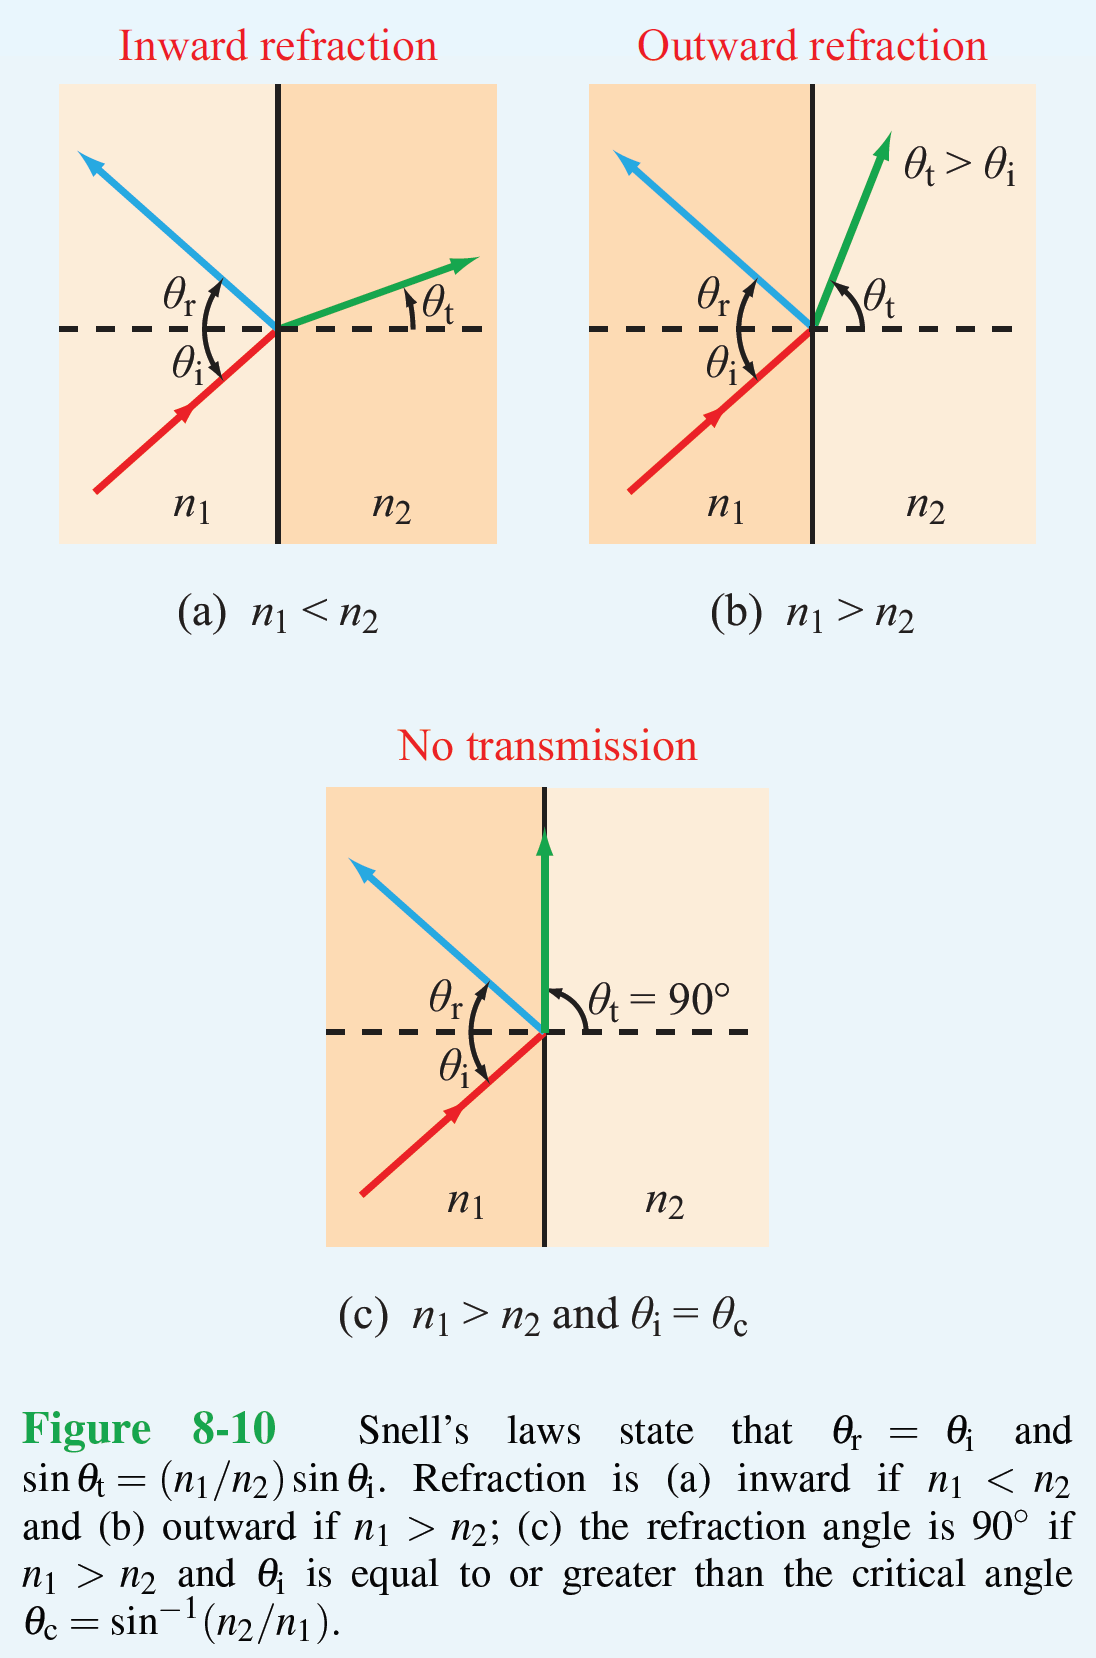
\includegraphics{Snell's laws and different angles.PNG}
    
\end{figure} 

\footnote{FAE - pag 350} 

\newpage 

\chapter{Onde piane TE e TM tra due materiali} 
\begin{figure}[h]
    \centering
    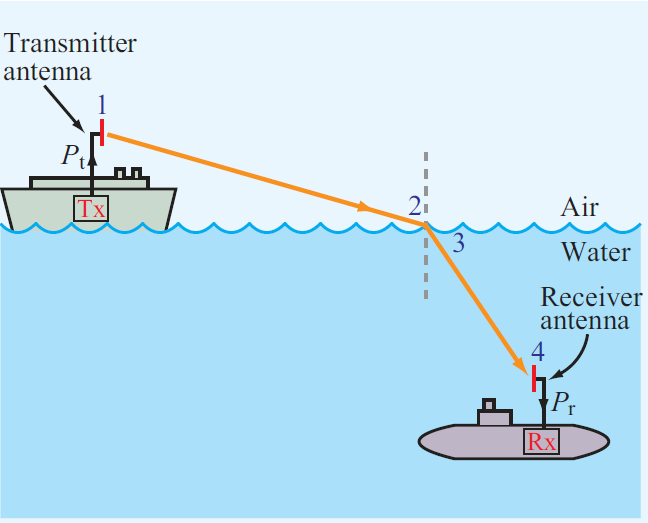
\includegraphics{TX and RX.PNG}
    
\end{figure}    

\newpage 

\section{Riflessione e trasmissione delle onde con incidenza obliqua} 

\footnote{FCE - pag 327 | 8.4 Riflessione e trasmissione delle onde con incidenza obliqua \\ 
FAE - pag 353 | 8.4 Wave reflectaion and trasmission at oblique incidence}

\begin{figure}[h]
    \centering
    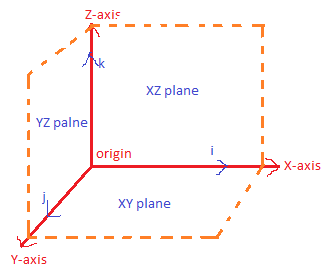
\includegraphics{x-z plane.jpeg}
    
\end{figure}  

\footnote{\url{https://www.vedantu.com/question-sets/0b332bea-6a22-4a13-971c-42e7b75218da6540201208005621542.png}}

Definiamo il piano (x-z); possiamo definire due tipi di polarizzazione: 

\begin{itemize}
    \item quando $\vec{E}$ è perpendicolare al piano (x-z), si definisce polarizzazione transversa elettrica (oppure polarizzazione TE)
    \item quando $\vec{H}$ è perpendicolare al piano (x-z), quindi $\vec{E}$ è parallelo al piano (x-z), viene definita come polarizzazione transversa magnetica (oppure polarizzazione TM)
\end{itemize}


Sia nel caso TE e TM, ricordiamo che, dato un piano di incidenza, le componenti tangenziali di $\vec{E}$ e $\vec{H}$ 
nei due piani devono essere continue. \\ 

\newpage 

\section{Onda piana TE} 

\footnote{FCE - pag 328 | 8.4.1 Polarizzazione perpendicolare \\ 
FAE - pag 354 | 8.4.1 Perpendicular Polarization} 

\begin{figure}[h]
    \centering
    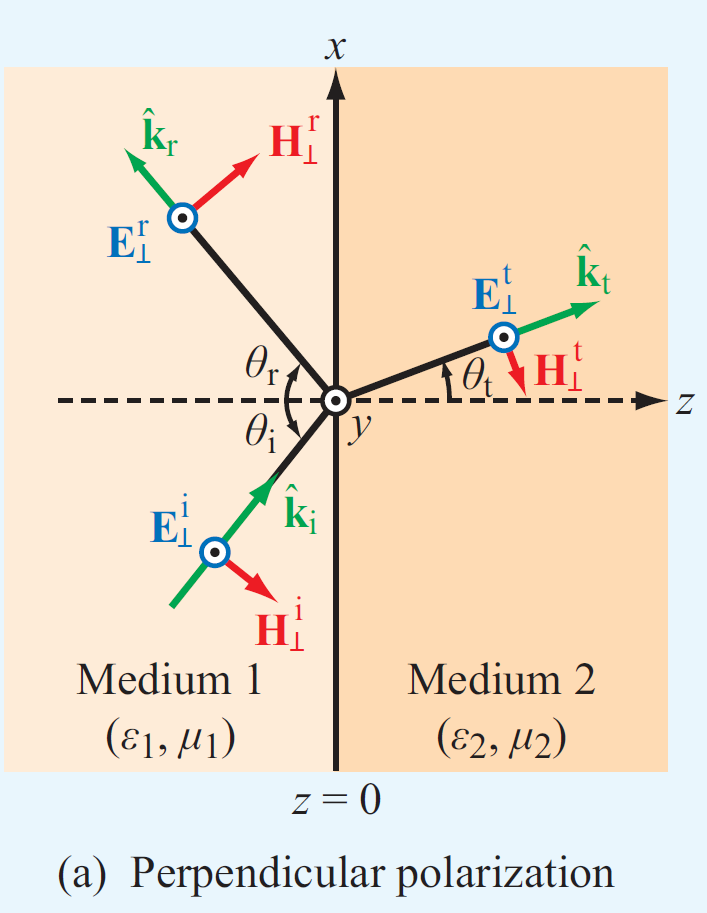
\includegraphics[scale = 0.8]{TE polarization.PNG}
    
\end{figure}    

\begin{figure}[h]
    \centering
    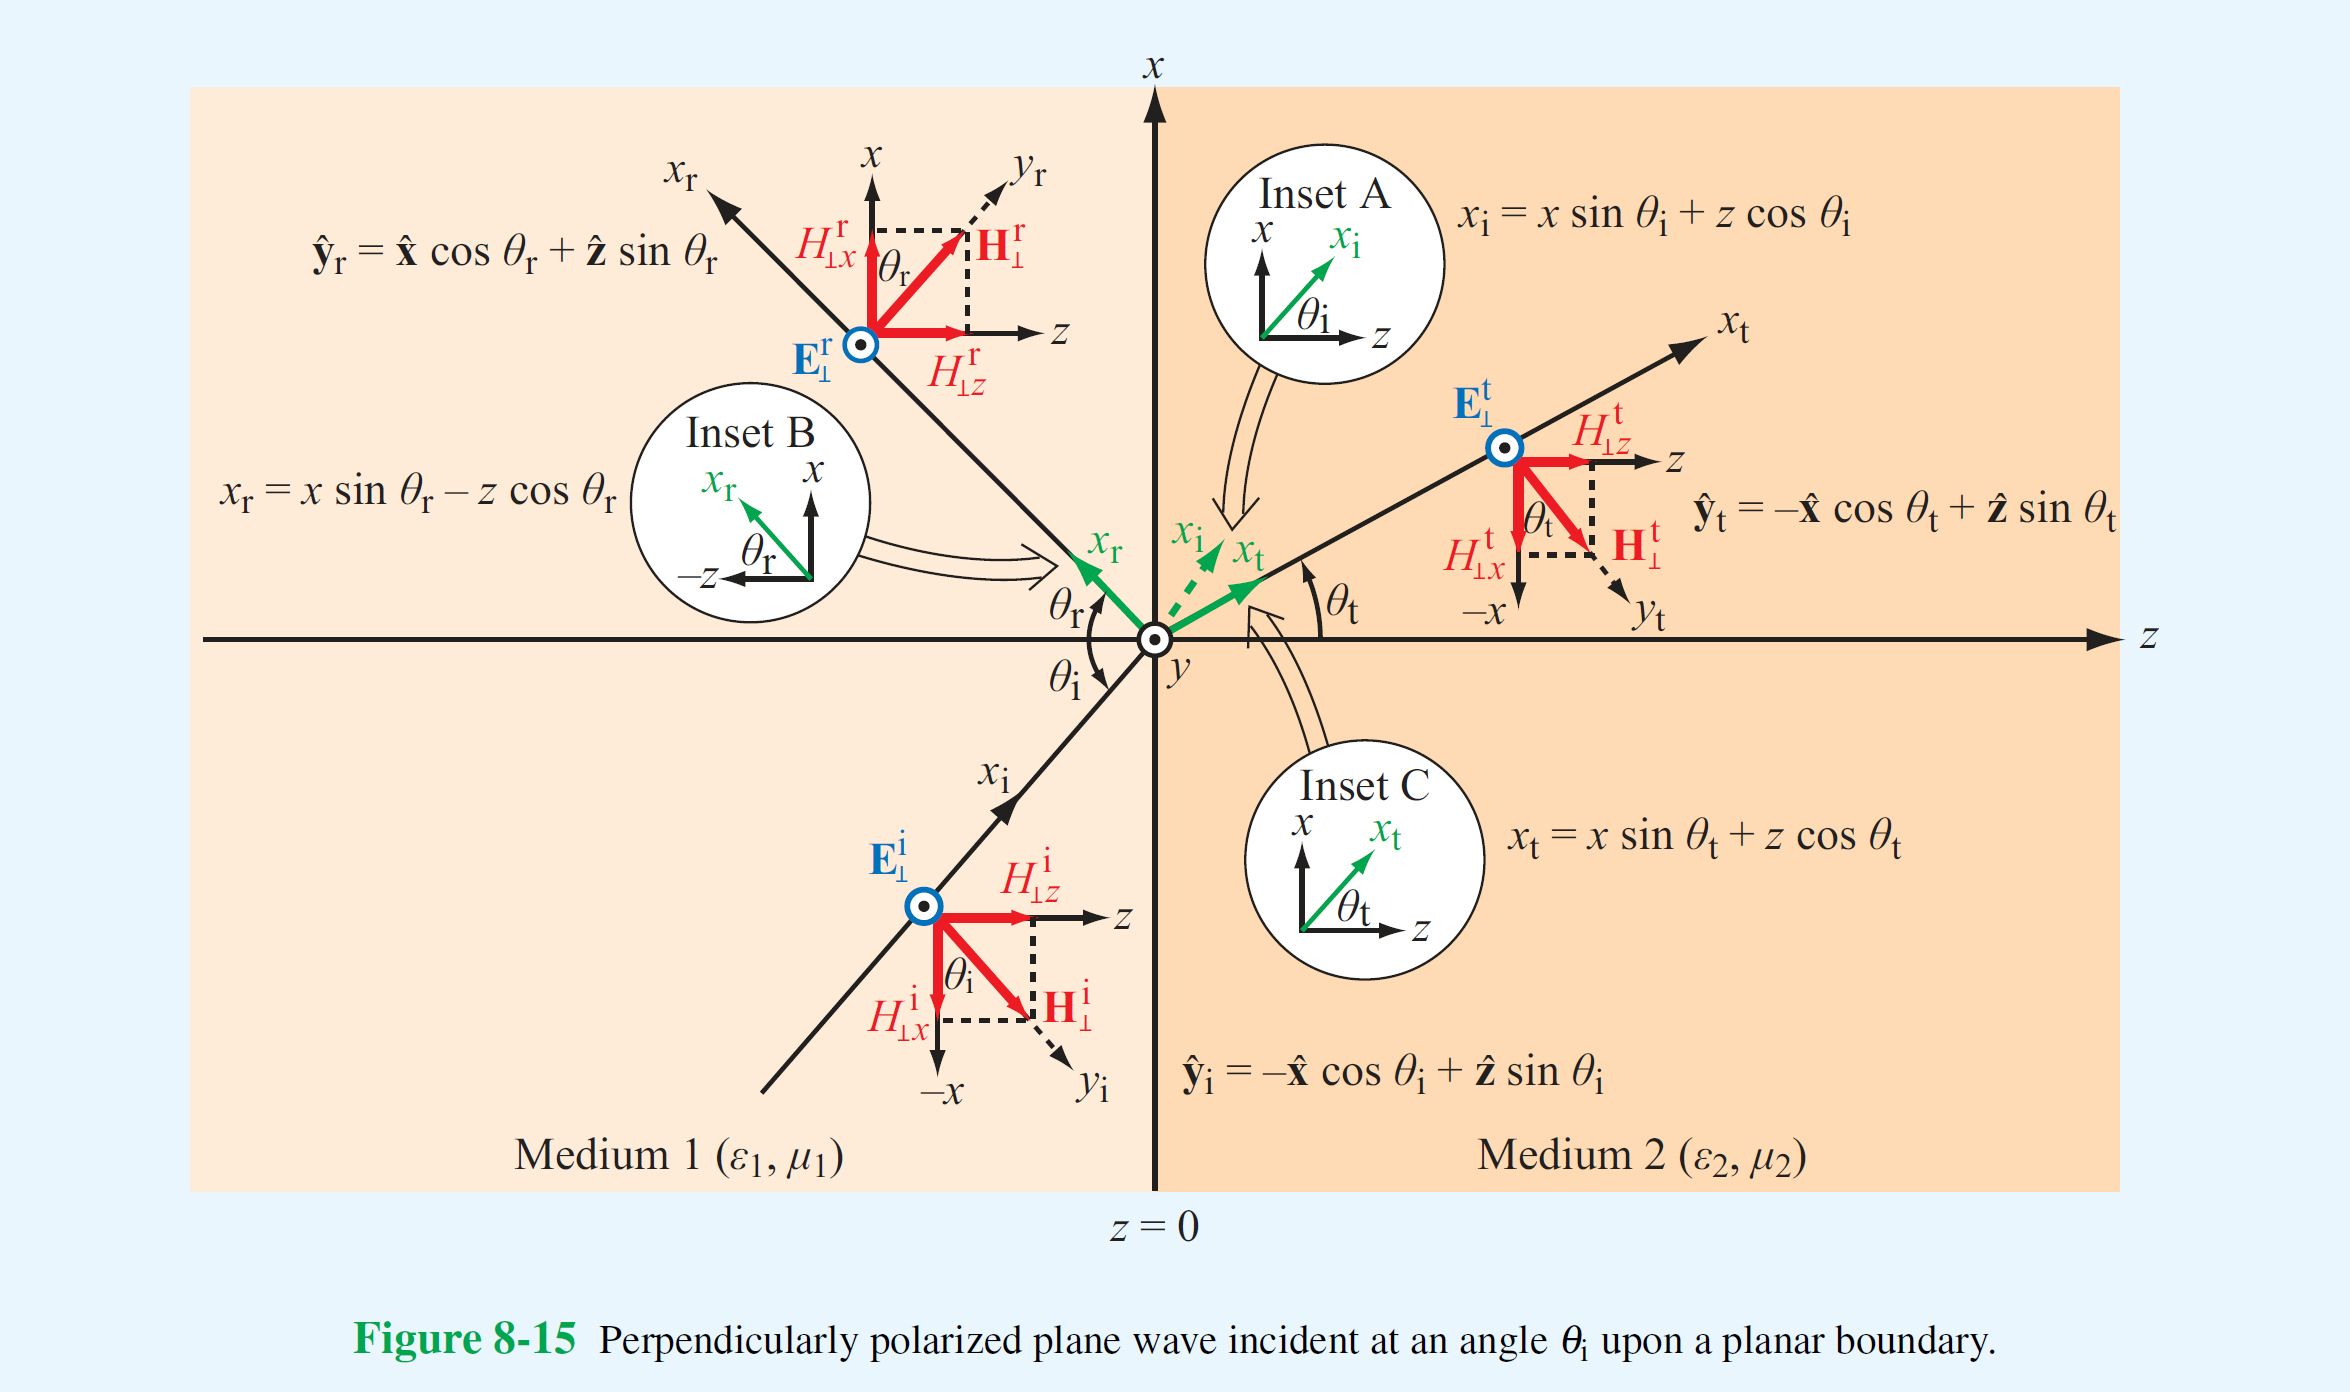
\includegraphics[scale = 0.5]{TE polarization with equations.PNG}
    
\end{figure}    

\footnote{FAE - pag 355} 

Nel mezzo 1 avremo: 

\begin{itemize}
    \item $\vec{E_\perp^{i}} $ punta in direzione $y$
    \item $\vec{H_\perp^{i}} $ punta in direzione $y_i$
\end{itemize}

Un'onda di questo tipo è descritta dalle seguenti equazioni: 

{\Large \begin{equation}
    \begin{cases}
        \vec{E_\perp^{1}} = \hat{y} E_{\perp_o}^{1} e^{-\jmath \kappa_1 x_i} \\ 
        \vec{H_\perp^{1}} = \hat{y_i} \frac{E_{\perp_o}^{1}}{\eta_1} e^{-\jmath \kappa_1 x_i}
    \end{cases}
\end{equation}}

dove: 

{\Large \begin{equation}
    \begin{cases}
        x_i = x \sin(\theta_i) + z \cos(\theta_i) \\ 
        \hat{y_i} = -\hat{x} \cos(\theta_i) + \hat{z} \sin(\theta_i)        
    \end{cases}
\end{equation}}

Scomponendo $\vec{E_\perp^{1}}$ in onda incidente e onda riflessa, avremo che: 

{\Large \begin{equation}
    \vec{E_\perp^{1}} = \vec{E_\perp^{i}} + \vec{E_\perp^{r}}
\end{equation}}

\textbf{Onda incidente:} 

{\Large \begin{equation}
    \begin{cases}
        \vec{E_\perp^{i}} = \hat{y} E_{\perp_o}^{i} e^{-\jmath \kappa_1 x_i} \\ 
        \vec{H_\perp^{i}} = \hat{y_i} \frac{E_{\perp_o}^{i}}{\eta_1} e^{-\jmath \kappa_1 x_i}
    \end{cases}
\end{equation}}

\textbf{Onda riflessa:} 

{\Large \begin{equation}
    \begin{cases}
        \vec{E_\perp^{r}} = \hat{y} E_{\perp_o}^{r} e^{-\jmath \kappa_1 x_r} \\ 
        \vec{H_\perp^{r}} = \hat{y_r} \frac{E_{\perp_o}^{r}}{\eta_1} e^{-\jmath \kappa_1 x_r}
    \end{cases}
\end{equation}}


dove: 

{\Large \begin{equation}
    \begin{cases}
        x_r = x \sin(\theta_r) - z \cos(\theta_r) \\ 
        \hat{y_r} = \hat{x} \cos(\theta_r) + \hat{z} \sin(\theta_r)        
    \end{cases}
\end{equation}}

Nel mezzo 2 avremo solo l'onda trasmessa. \\ 

\textbf{Onda trasmessa:} 

{\Large \begin{equation}
    \begin{cases}
        \vec{E_\perp^{t}} = \hat{y} E_{\perp_o}^{t} e^{-\jmath \kappa_2 x_t} \\ 
        \vec{H_\perp^{t}} = \hat{y_t} \frac{E_{\perp_o}^{t}}{\eta_2} e^{-\jmath \kappa_2 x_t}
    \end{cases}
\end{equation}}

dove: 

{\Large \begin{equation}
    \begin{cases}
        x_t = x \sin(\theta_t) + z \cos(\theta_t) \\ 
        \hat{y_t} = -\hat{x} \cos(\theta_t) + \hat{z} \sin(\theta_t)        
    \end{cases}
\end{equation}}


Dal momento che i campi elettrici nel mezzo 1 e nel mezzo 2 presentano solo componenti 
lungo $\hat{y}$, la condizione al contorno di $\vec{E}$ è: 

{\Large \begin{equation}
    (\vec{E_{\perp_y}^{i}} + \vec{E_{\perp_y}^{r}} )\big|_{z=0} = 
    \vec{E_{\perp_y}^{t}}\big|_{z=0}
\end{equation}} 

\begin{tcolorbox}
    Il simbolo matematico $\big|$ indica che l'equazone e/o la formula a sinistra del segno 
    viene calcolata, o propriamente si dice valutata, nel punto inidicato in basso a destra del segno. \\ \\
    Per esempio: \\ 

    $\vec{E_{\perp_y}^{t}}\big|_{z=0}$ \\ 

    si legge: \\ 
    la componete y del vettore del campo elettrico con polarizzazione TE trasmessa nella regione 2 
    viene valutata nel punto $z=0$ 
\end{tcolorbox}

Svolgendo diversi passaggi algebrici, avremo che: 

{\Large \begin{equation}
    E_{\perp_o}^{i} e^{-\jmath \kappa_1 x \sin(\theta_i)} + E_{\perp_o}^{r} e^{-\jmath \kappa_1 x \sin(\theta_r)} = 
    E_{\perp_o}^{t} e^{-\jmath \kappa_2 \sin(\theta_t)}
\end{equation}}

La condizione al contorno del campo elettrico (cioè il campo lungo x) è: 

{\Large \begin{equation}
    (\vec{H_{\perp_x}^{i}} + \vec{H_{\perp_x}^{r}} )\big|_{z=0} = 
    \vec{H_{\perp_x}^{t}}\big|_{z=0}
\end{equation}} 

In formule: 

{\Large \begin{equation}
    - \frac{E_{\perp_o}^{i}}{\eta_1} \cos(\theta_i) e^{-\jmath \kappa_1 \sin(\theta_i)} + \frac{E_{\perp_o}^{r}}{\eta_1} \cos(\theta_r) e^{-\jmath \kappa_1 \sin(\theta_r)} = 
    - \frac{E_{\perp_o}^{t}}{\eta_2} \cos(\theta_t) e^{-\jmath \kappa_2 \sin(\theta_t)}    
\end{equation}}


Per soddisfare le due condizioni al contorno per ogni valore di x, tutti gli argomenti degli esponenziali devono essere uguali, quindi: 

{\Large \begin{equation}
    \kappa_1 \sin(\theta_i) = \kappa_1 \sin(\theta_r) = \kappa_2 \sin(\theta_t) 
\end{equation}}

Questa triplice uguaglianza è detta condizione di phase-matching. \\ 

Sapendo che $\theta_i = \theta_r$ e applicando il phase-matching, avremo che: 

{\Large \begin{equation}
    E_{\perp_o}^{i} + E_{\perp_o}^{r} = E_{\perp_o}^{t} 
\end{equation}} 

Cioè: 

{\Large \begin{equation}
    \frac{\cos(\theta_i)}{\eta_1} (- E_{\perp_o}^{i} + E_{\perp_o}^{r}) = 
    - \frac{\cos(\theta_t)}{\eta_2} E_{\perp_o}^{t}
\end{equation}}

Da queste due equazioni, è possibile ricavare, come il caso TEM, il coefficiente di riflessione e di trasmissione. 

{\Large \begin{equation}
    \Gamma_{TE} = \frac{E_{\perp_o}^{r}}{E_{\perp_o}^{i}} = \frac{\eta_2 \cos(\theta_i) - \eta_1 \cos(\theta_t)}{\eta_2 \cos(\theta_i) + \eta_1 \cos(\theta_t)}
\end{equation}}


\begin{tcolorbox}
    Nel caso TEM: \\ \\ $\Gamma_{TEM} = \frac{\eta_2 - \eta_1}{\eta_2 + \eta_1}$
\end{tcolorbox}


{\Large \begin{equation}
    \tau_{TE} = \frac{E_{\perp_o}^{t}}{E_{\perp_o}^{i}} = \frac{2 \eta_2 \cos(\theta_i) }{\eta_2 \cos(\theta_i) + \eta_1 \cos(\theta_t)}
\end{equation}}


\begin{tcolorbox}
    Nel caso TEM: \\ \\ $\tau_{TEM} = \frac{2 \eta_2}{\eta_2 + \eta_1}$
\end{tcolorbox}

I due coefficienti sono legati da: 

{\Large \begin{equation}
    \tau_{TE} = 1 + \Gamma_{TE} 
\end{equation}}

Utilizzando i coefficienti, possiamo scrivere la continuità in $z=0$ sapendo il valore di $E_{\perp_o}^{i} = E_1$ come: 

{\Large \begin{equation}
    E_1 \cos(1 + \Gamma_{TE}) = \tau_{TE} E_1 \cos(\theta_2)
\end{equation}} 

Diventa: 

{\Large \begin{equation}
    \frac{E_1}{\eta_1} (1 + \Gamma_{TE}) = \tau_{TE} \frac{E_2}{\eta_2}
\end{equation}} 


Se il mezzo 2 è un perfetto conduttore ($\eta_2 = 0$), allora $\Gamma_{TE} = -1$ e $\tau_{TE} = 0$. \\ 

Ricordiamo che per materiali non magneitici, $\mu_1 = \mu_2 = \mu_o$, quindi si può esprimere $\Gamma_{TE}$ grazie 
a queste sostituzioni. 


\newpage 

\section{Onda piana TM}

\footnote{FCE - pag 333 | Polarizzazione parallela \\ 
FAE - pag 359 | 8.4.2 Parallel Polarization} 

\begin{figure}[h]
    \centering
    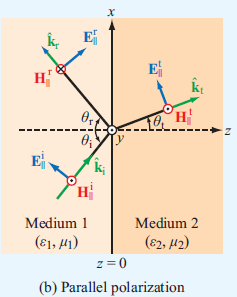
\includegraphics[scale = 0.8]{TM polarization.PNG}
    
\end{figure}   

\footnote{FAE - pag 354 } 

\begin{figure}[h]
    \centering
    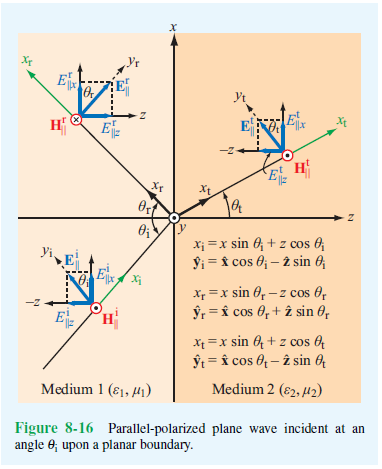
\includegraphics[scale = 0.8]{TM polarization with equations.PNG}
    
\end{figure}   

Stesso principio della polarizzazione perpendicolare TE, quindi: 

{\Large \begin{equation}
    \begin{cases}
        \vec{E_\parallel^{1}} = \vec{E_\parallel^{i}} + \vec{E_\parallel^{r}} \\ 
        \vec{H_\parallel^{1}} = \vec{H_\parallel^{i}} + \vec{H_\parallel^{r}}
    \end{cases}
\end{equation}}


\textbf{Onda incidente:} 

{\Large \begin{equation}
    \begin{cases}
        \vec{E_\parallel^{i}} = \hat{y_i} E_{\parallel_o}^{i} e^{-\jmath \kappa_1 x_i} \\ 
        \vec{H_\parallel^{i}} = \hat{y} \frac{E_{\parallel_o}^{i}}{\eta_1} e^{-\jmath \kappa_1 x_i}
    \end{cases}
\end{equation}} 

dove: 

{\Large \begin{equation}
    \begin{cases}
        x_i = x \sin(\theta_i) + z \cos(\theta_i) \\ 
        \hat{y_i} = \hat{x} \cos(\theta_i) - \hat{z} \sin(\theta_i)        
    \end{cases}
\end{equation}}

\textbf{Onda riflessa:} 

{\Large \begin{equation}
    \begin{cases}
        \vec{E_\parallel^{r}} = \hat{y_r} E_{\parallel_o}^{r} e^{-\jmath \kappa_1 x_r} \\ 
        \vec{H_\parallel^{r}} = - \hat{y} \frac{E_{\parallel_o}^{r}}{\eta_1} e^{-\jmath \kappa_1 x_r}
    \end{cases}
\end{equation}} 

dove: 

{\Large \begin{equation}
    \begin{cases}
        x_r = x \sin(\theta_r) - z \cos(\theta_r) \\ 
        \hat{y_r} = \hat{x} \cos(\theta_r) + \hat{z} \sin(\theta_r)        
    \end{cases}
\end{equation}}


\textbf{Onda trasmessa:} 

{\Large \begin{equation}
    \begin{cases}
        \vec{E_\parallel^{t}} = \hat{y_t} E_{\parallel_o}^{t} e^{-\jmath \kappa_2 x_t} \\ 
        \vec{H_\parallel^{t}} = \hat{y} \frac{E_{\parallel_o}^{t}}{\eta_2} e^{-\jmath \kappa_2 x_t}
    \end{cases}
\end{equation}} 

dove: 

{\Large \begin{equation}
    \begin{cases}
        x_t = x \sin(\theta_t) + z \cos(\theta_t) \\ 
        \hat{y_t} = \hat{x} \cos(\theta_t) - \hat{z} \sin(\theta_t)        
    \end{cases}
\end{equation}}

Facendo la stessa cosa che abbiamo fatto con la polarizzazione TE per la continuità dei 
componenti trasversali di $\vec{E}$ e $\vec{H}$ in $z=0$, possiamo ricavarci i coeffienti di Fresnel per la polarizzazione parallela. 

{\Large \begin{equation}
    \Gamma_{TM} = \frac{E_{\parallel_o}^{r}}{E_{\parallel_o}^{i}} = \frac{\eta_2 \cos(\theta_t) - \eta_1 \cos(\theta_i)}{\eta_2 \cos(\theta_t) + \eta_1 \cos(\theta_i)}
\end{equation}}

{\Large \begin{equation}
    \tau_{TM} = \frac{E_{\parallel_o}^{t}}{E_{\parallel_o}^{i}} = \frac{2 \eta_2 \cos(\theta_i) }{\eta_2 \cos(\theta_t) + \eta_1 \cos(\theta_i)}
\end{equation}} 

Si può dimostrare che: 

{\Large \begin{equation}
    \tau_{TM} = (1 + \Gamma_{TM}) \frac{\cos(\theta_i)}{\cos(\theta_t)} 
\end{equation}} 


Come il caso TE, se il mezzo 2 è un perfetto conduttore ($\eta_2 = 0$), allora $\Gamma_{TM} = -1$ e $\tau_{TM} = 0$. \\ 

Ricordiamo che per materiali non magneitici, $\mu_1 = \mu_2 = \mu_o$, quindi si può esprimere $\Gamma_{TM}$ grazie 
a queste sostituzioni. 


\newpage 

\section{Angolo di Brewster} 

\footnote{FCE - pag 335 | 8.4.3 Angolo di Brewster \\ 
FAE - pag 360 | 8.4.3 Brewster angle } 

L'angolo di Brewster $\theta_B$ è definito come l'angolo di incidenza $\theta_i$ per il quale $\Gamma = 0$. \\ 

Dalla definizione di $\Gamma_{TE}$: 

{\Large \begin{equation}
    \Gamma_{TE} = \frac{E_{\perp_o}^{r}}{E_{\perp_o}^{i}} = \frac{\eta_2 \cos(\theta_i) - \eta_1 \cos(\theta_t)}{\eta_2 \cos(\theta_i) + \eta_1 \cos(\theta_t)}
\end{equation}}

{\Large \begin{equation}
    \Gamma_{TE} = 0 \iff \eta_2 \cos(\theta_i) - \eta_1 \cos(\theta_t) = 0 
    \iff \eta_2 \cos(\theta_i) = \eta_1 \cos(\theta_t)
\end{equation}} 


\begin{tcolorbox}
    $\iff$ è il simbolo matematico per dire "se e solo se"
\end{tcolorbox}

Facendo le dovute sostituzioni (omesse per semplicità) a $\Gamma_{TE}$ avremo che: 

{\Large \begin{equation}
    \sin(\theta_{B_{TE}}) = \sqrt{\frac{1 - \frac{\mu_1 \varepsilon_2}{\mu_2 \varepsilon_1}}{1 - (\frac{\mu_1}{\mu_2} )^{2}}}
\end{equation}} 

Per materiali non magneitici, $\mu_1 = \mu_2 $ quindi il denominatore della divisione è $=0$, 
quindi $\theta_{B_{TE}}$ non esiste. \\ \\ 

Per le onde TM, si fa lo stesso procedimento e avremo che: 

{\Large \begin{equation}
    \sin(\theta_{B_{TM}}) = \sqrt{\frac{1 - \frac{\mu_2 \varepsilon_1}{\mu_1 \varepsilon_2}}{1 - (\frac{\varepsilon_1}{\varepsilon_2} )^{2}}}
\end{equation}} 

Per materiali non magneitici, $\mu_1 = \mu_2$ quindi: 

{\Large \begin{equation}
    \begin{split}
        \theta_{B_{TM}} 
        &= \arcsin(\sqrt{\frac{1}{1 + \frac{\varepsilon_1}{\varepsilon_2}}}) 
        \\
        &= \arctan (\sqrt{\frac{\varepsilon_2}{\varepsilon_1}}) 
    \end{split}
\end{equation}}

\begin{tcolorbox}
    $\arcsin = \sin ^{-1}$ cioè l'inverso della funzione $\sin$
\end{tcolorbox}



\footnote{Slide prof | Incidenza obliqua su un piano di massa | Pag 20}

L'angolo di Brewster viene definito anche come angolo polizzatore perchè se un'onda non polarizzata (quindi 
contiene sia un'onda TE che TM) è incidente a $\theta_{B_{TM}}$, allora la componente TM passa nel mezzo 2, 
mentre la componente TE viene riflessa e polarizzata. 


\begin{figure}[h]
    \centering
    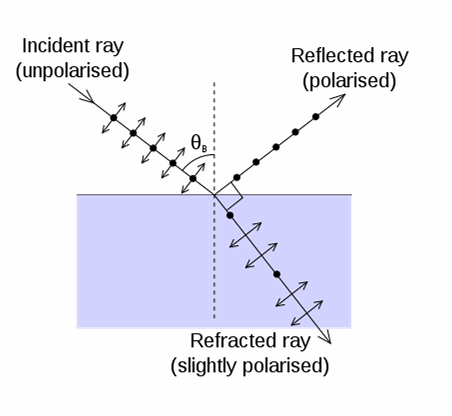
\includegraphics[scale = 0.3]{Angolo polarizzatore.PNG}
    
\end{figure}  

\newpage

\section{Vettore di Poynting per onde TE e TM} 

\footnote{FCE - pag 337 | 8.5 Riflettività e trasmissitività \\ 
FAE - pag 361 | 8.5 Reflectivity and Trasmissitivity}

\begin{figure}[h]
    \centering
    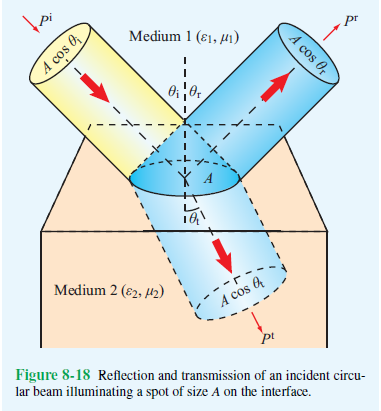
\includegraphics[scale = 0.8]{Vettore Poynting TE e TM.PNG}
    
\end{figure}  

Consideriamo le onde con polarizzazione TE. \\ 

La densità di potenza dei fasci incidente, riflesso e trasmesso sono: 

{\Large \begin{equation}
    \begin{cases}
        S_\perp ^{i} = \frac{\left|E_{\perp_o} ^{i}\right| ^{2}}{2 \eta_1} \\ 
        S_\perp ^{r} = \frac{\left|E_{\perp_o} ^{r}\right| ^{2}}{2 \eta_1} \\ 
        S_\perp ^{t} = \frac{\left|E_{\perp_o} ^{t}\right| ^{2}}{2 \eta_2}
    \end{cases}
\end{equation}}


Consideriamo A come la regione illuminata dalle onde, avremo: 

{\Large \begin{equation}
    \begin{cases}
        A_i = A \cos(\theta_i) \\ 
        A_r = A \cos(\theta_r) \\ 
        A_t = A \cos(\theta_t)  
    \end{cases}
\end{equation}}

Le potenze medie trasportate dalle onde saranno: 

{\Large \begin{equation}
    \begin{cases}
        P_{TE} ^{i} = S_\perp ^{i} A_i = \frac{\left|E_{\perp_o} ^{i}\right| ^{2}}{2 \eta_1} A \cos(\theta_i) \\ 
        P_{TE} ^{r} = S_\perp ^{r} A_r = \frac{\left|E_{\perp_o} ^{i}\right| ^{2}}{2 \eta_1} A \cos(\theta_r) \\ 
        P_{TE} ^{t} = S_\perp ^{t} A_t = \frac{\left|E_{\perp_o} ^{t}\right| ^{2}}{2 \eta_2} A \cos(\theta_t) 
    \end{cases}
\end{equation}}

Definiamo R come indice di riflettanza: 

{\Large \begin{equation}
    R_{TE} = \frac{P_{TE} ^{r}}{P_{TE} ^{i}} = \frac{\left|E_{\perp_o} ^{r}\right| ^{2} \cos(\theta_r)}{\left|E_{\perp_o} ^{i}\right| ^{2} \cos(\theta_i)} = \left|\frac{E_{\perp_o} ^{r}}{E_{\perp_o} ^{i}}\right| ^{2} = \left|\Gamma_\perp\right|\ ^{2}  
\end{equation}}

in cui $\theta_r = \theta_i$. \\ 

Indichiamo con T la trasmittanza: 

{\Large \begin{equation}
    T_{TE} = \frac{P_\perp ^{t}}{P_\perp ^{i}} = \frac{\left|E_{\perp_o} ^{t}\right| ^{2}}{\left|E_{\perp_o} ^{i}\right| ^{2}} \frac{\eta_1}{\eta_2} \frac{A \cos(\theta_t)}{A \cos(\theta_i)} = 
    \left|\tau_{TE}\right| ^{2} (\frac{\eta_1 \cos(\theta_t)}{\eta_2 \cos(\theta_i)})
\end{equation}}

Come il caso TE, possiamo esprimere la riflettanza e la trasmittanza nel caso TM: 

{\Large \begin{equation}
    \begin{cases}
        R_{TM} = \frac{P_{TM} ^{r}}{P_{TM} ^{i}} = \left|\Gamma_{TM}\right| ^{2} \\ 
        T_{TM} = \frac{P_{TM} ^{t}}{P_{TM} ^{i}} = \left|\tau_{TM}\right| ^{2}  (\frac{\eta_1 \cos(\theta_t)}{\eta_2 \cos(\theta_i)})
    \end{cases}    
\end{equation}}

Possiamo dire che, per la converzione dell'energia. che: 

{\Large \begin{equation}
    P_{TE} ^{i} = P_{TE} ^{r} + P_{TE} ^{t} 
\end{equation}} 

cioè: 

{\Large \begin{equation}
    \begin{cases}
        R_\perp + T_\perp = 1 \\ 
        R_\parallel + T_\parallel = 1 
    \end{cases}
\end{equation}} 


Per $\theta_B$, $R_{TM} = 0$ e $\tau_{TM} = 1$. \\ \\ 

Per riassumere: 

\begin{figure}[h]
    \centering
    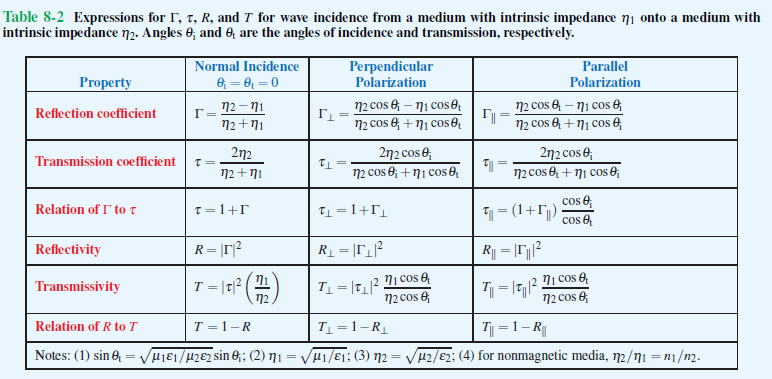
\includegraphics[scale = 0.8]{Tabella coefficienti onde piane.PNG}
    
\end{figure}  

\footnote{FAE - pag 363} 

\newpage 


 

\chapter{Cavo Coax}

\begin{figure}[h]
    \centering
    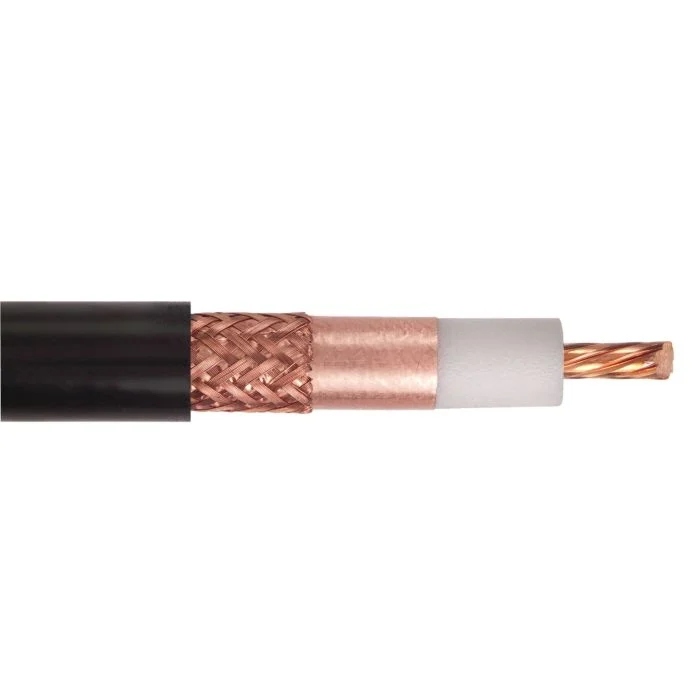
\includegraphics[scale = 0.5]{cavo coassiale vero.png}
\end{figure} 

\newpage 

\section{Campo EM in un cavo coax} 

\footnote{Slide del prof | PPT: Lezione 16 Mezzi trasmissivi 03 Maggio 23 | Pag 3-13}

\begin{figure}[h]
    \centering
    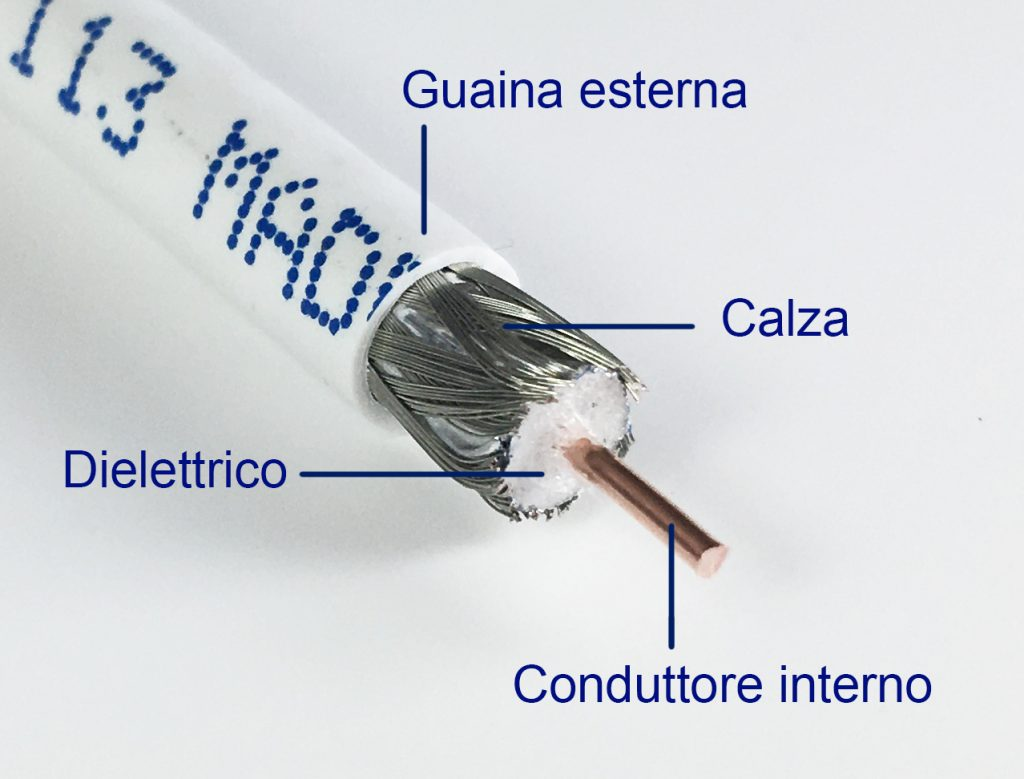
\includegraphics[scale = 0.5]{Cavo-spelato-nomi-delle-parti-copia-1024x779.jpg}
\end{figure} 

\footnote{\url{https://www.sistemi-integrati.net/cose-un-cavo-coassiale/}} 

Il cavo coassiale è un cavo cilindrico formato da (dall'interno all'esterno): 

\begin{itemize}
    \item condutore interno 
    \item dielettrico di separazione 
    \item calza conduttrice coassiale 
    \item guaina di protezione 
\end{itemize}

Essendo il cavo coassiale fisicamente di forma cilindrica, 
possiamo usare i fasori, in particolare le equazioni di Maxwell in forma 
fasoriale in assenza di sorgenti: 

{\Large \begin{equation}
    \begin{cases}
        \nabla \cdot \vec{E} = 0 \\ 
        \nabla \cdot \vec{H} = 0 \\
        \nabla \times \vec{E} = - \jmath \omega \mu \vec{H} \\ 
        \nabla \times \vec{H} = \jmath \omega \varepsilon \vec{E} 
    \end{cases}
\end{equation}}

Nella realtà non possiamo esprimere le equazioni delle onde in un cavo coassiale 
con le equazioni di Maxwell in assenza di sorgenti, ma adesso ci poniamo nel caso più 
semplice per svolgere i calcoli. \\ 

Sempre per quest'ultimo principio, consideriamo le onde polarizzate TEM, quindi: 

{\Large \begin{equation}
    \begin{cases}
        E_z = 0 \\ 
        H_z = 0
    \end{cases}
\end{equation}}

Considerando il cavo coassiale come cilindro, possiamo esprimere ogni punto del cavo 
in coordinate cilindriche: 

{\Large \begin{equation}
    (x, y, z) \Rightarrow (r, \phi, z )
\end{equation}}

\begin{tcolorbox}
    Dall'analisi matematica: 
    \begin{itemize}
        \item r indica il raggio 
        \item $\phi$ (si legge fi) indica i gradi  
    \end{itemize}
    Per approfondire\\
    \url{https://www.youmath.it/lezioni/analisi-due/varie/2282-coordinate-cilindriche.html} \\ 

    In questa sezione la notazione dei vettori indica quella di un fasore. 
\end{tcolorbox}

Vogliamo trovare una soluzione che non dipenda 
da $\phi$, quindi:
{\Large \begin{equation}
    \frac{\partial}{\partial \phi} = 0
\end{equation}} 

Essendo 
{
    \Large
     \begin{equation}
  E_z = 0      
     \end{equation}
}

$E_z$ è indipendete da $\phi$: 
questo principio prende il nome di simmetria azimutale. \\ 

Quindi possiamo scrivere che: 

{\Large \begin{equation}
    \nabla \cdot \vec{E} = 0 = \frac{1}{r} \frac{\partial}{\partial r} (r \vec{E_r} (r, z) )
\end{equation}}

Da questa equazione, notiamo che $\vec{E}$ dipende da r e da z. \\ 

Ritornando alla forma fisica del cavo coassiale, 
abbiamo due conduttori (il conduttore interno e la calza conduttrice coassiale) divisi 
da un dielettrico, proprio come un condensatore. \\ 

\begin{tcolorbox}
    Per approfondori sui condensatori \\
    \url{https://www.elettra2000.it/vdegliesposti/Dispense%20Propagazione/Richiami_Teoria_Dei_Circuiti.pdf}
\end{tcolorbox}
 
Applicando l'equazione costitutiva del condensatore al cavo coassiale, avremo che: 

{\Large \begin{equation}
    r \vec{E_r} (r, z) = Costante \cdot \vec{V} (z) 
    \Rightarrow \vec{E_r} (r, z) = \frac{Costante}{r} \vec{V} (z) 
\end{equation}}


\begin{figure}[h]
    \centering
    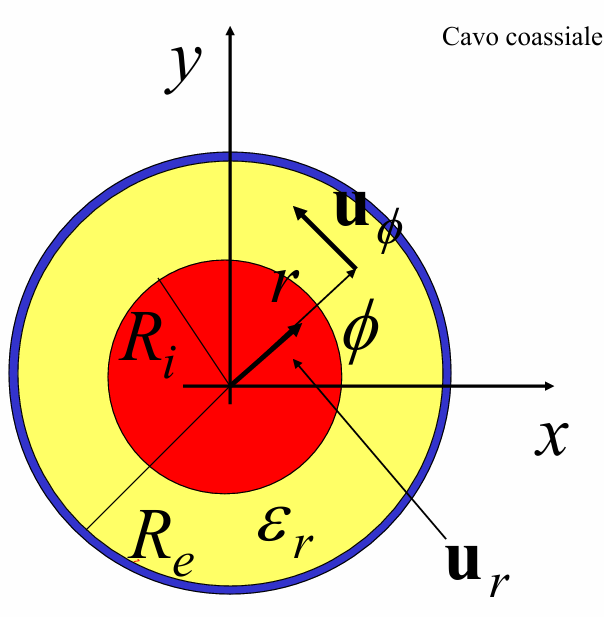
\includegraphics[scale = 0.5]{Cavo coax schematizzato.PNG}
\end{figure} 

\footnote{Slide del prof | PPT: Lezione 16 Mezzi trasmissivi 03 Maggio 23 | Pag 5} 

Proprio come il condensatore, facciamo un'intergrale di linea di un percorso chiuso tra le due armature, 
in questo caso tra i due conduttori: 

{\Large \begin{equation}
    \begin{split}
        \int_{R_i}^{R_e} \vec{E_r}(r, z) dr &= 
        \int_{R_i}^{R_e} \frac{Costante}{r} \vec{V} (z) dr \\
        & =  Costante \cdot \vec{V} (z) \int_{R_i}^{R_e} \frac{1}{r} dr \\ 
        & = Costante \cdot \vec{V} (z) \cdot \ln \left|r\right| \big|_{R_i} ^{R_e}   \\ 
        & =  Costante \cdot \vec{V} (z) \cdot \ln \left|R_e\right| - \\ 
        & Costante \cdot \vec{V} (z) \cdot \ln \left|R_i\right|  \\ 
        & = Costante \cdot \vec{V} (z) (\ln \left|R_e\right| - \ln \left|R_i\right|)  \\ 
        & = Costante \cdot \vec{V} (z) \ln \left|\frac{R_e}{R_i}\right|
    \end{split}
\end{equation}}

\begin{tcolorbox}
    $Costante \cdot \vec{V} (z)$ \\ 
    possiamo portarlo subito fuori dall'intergrale perchè 
    sono costanti rispetto a dr (r è l'incognita dell'integrale)   
\end{tcolorbox}

Alla fine avremo: 

{\Large \begin{equation}
    Costante \cdot \vec{V} (z) \ln \left|\frac{R_e}{R_i}\right| = \vec{V} (z)
\end{equation}}

Per essere vera questa ultima equazione: 

{\Large \begin{equation}
    Costante = \frac{1}{\ln \left|\frac{R_e}{R_i}\right|}
\end{equation}}

Sapendo ora il valore della costante possiamo esprimere $\vec{E_r}$ come: 

{\Large \begin{equation}
    \vec{E_r} (r, z) = \frac{Costante}{r} \vec{V} (z) 
    \Rightarrow \vec{E_r} (r, z) = \frac{1}{\ln \left|\frac{R_e}{R_i}\right|}  \frac{\vec{V} (z)}{r}
\end{equation}}

In "2.1 Equazioni dell'onda in forma fasoriale", abbiamo trovato che: 

{\Large \begin{equation}
    H_y = \frac{1}{- \jmath \omega \mu} \frac{\partial E_x}{\partial z}
\end{equation}}

In coordinate cilindriche, possiamo sostituire le rispettive coordinate, 
quindi $H_y$ diventa: 

{\Large \begin{equation}
    \vec{H_\phi} = \frac{1}{- \jmath \omega \mu} \frac{\partial E_r}{\partial z}
\end{equation}}

Sostitendo il valore di $\vec{E_r}$ trovato precedentemente, $\vec{H_\phi}$ diventa: 

{\Large \begin{equation}
    \vec{H_\phi} = \frac{1}{- \jmath \omega \mu} \frac{1}{r \ln \left|\frac{R_e}{R_i}\right| }\frac{\partial \vec{V} (z)}{\partial z}
\end{equation}}

Ritornando alle equazioni in forma fasoriale in coordinate cartesiane, sapevamo che: 

{\Large \begin{equation}
    \nabla \times \vec{H} = \jmath \omega \varepsilon \vec{E} 
    \Rightarrow \vec{E} = \frac{1}{\jmath \omega \varepsilon} \nabla \times \vec{H}
\end{equation}}

Sapendo il valore di $\vec{H}$, nell'asse x abbiamo che: 

{\Large \begin{equation}
    - \frac{\partial H_y}{\partial z} = \jmath \omega \varepsilon E_x 
    \Rightarrow E_x = - \frac{\partial H_y}{\partial z} \cdot \frac{1}{\jmath \omega \varepsilon}
\end{equation}}

Sostitendo a $x \Rightarrow r$ e $y \Rightarrow \phi$, avremo che: 

{\Large \begin{equation}
    \vec{E_r} (r, z) = - \frac{\partial H_\phi}{\partial z} \cdot \frac{1}{\jmath \omega \varepsilon}
\end{equation}}

Sapendo il valore di $H_\phi$, possiamo esprimere $\vec{E_r} (r, z)$ come: 

{\Large \begin{equation}
    \vec{E_r} (r, z) = - \frac{1}{r \ln \left|\frac{R_e}{R_i}\right|} \frac{1}{\kappa^{2}} \frac{\partial ^{2} \vec{V} (z)}{\partial  z^{2}}
\end{equation}}

Quindi è un'equazione che soddisfa l'equazione dell'onda: 

{\Large \begin{equation}
    \nabla ^{2} \vec{E} = -\kappa ^{2} \vec{E}
\end{equation}} 

dove: 

{\Large \begin{equation}
    \kappa ^{2} = \omega ^{2} \mu \varepsilon
\end{equation}} 

\newpage 

\section{Campo EM nel tempo}

\footnote{Slide del prof | PPT: Lezione 16 Mezzi trasmissivi 03 Maggio 23 | Pag 14 - 23}

Siccome le equazioni del campo EM soddisfano l'equazione dell'onda, 
possiamo esprimere la tensione come una sinusoide del tipo: 


{\Large  \begin{equation}
    \vec{E} (z) = V^{+} e^{-\jmath \kappa z} + V^{-} e^{+\jmath \kappa z}    
\end{equation}}


Ricordando che: 

{\Large \begin{equation}
    \vec{V} (z) = - \frac{1}{\kappa ^{2}} \frac{\partial^{2} \vec{V} (z)}{\partial z^{2}}
\end{equation}} 

e che: 

{\Large \begin{equation}
    \vec{E_r} (r, z) = \frac{1}{r \ln \left|\frac{R_e}{R_i}\right|} \vec{V}(z)
\end{equation}}

allora, possiamo convertire i fasori in quantità che variano nel tempo: 

{\Large \begin{equation}
    \begin{split}
        \Re{\vec{E_r} (r, z) e^{\jmath \kappa z}} 
        &= \frac{1}{r \ln \left|\frac{R_e}{R_i}\right|} \Re{\vec{V} (z) e^{\jmath \kappa z}} \\
        &= \frac{1}{r \ln \left|\frac{R_e}{R_i}\right|} V(z, t)
    \end{split}
\end{equation}}

dove: 

{\Large \begin{equation}
    \begin{split}
        V(z, t) 
        &=  \Re{\vec{V} (z) e^{\jmath \kappa z}} \\ 
        &= V^{+} \cos(\omega t - \kappa z) + V^{-} \cos(\omega t + \kappa z)     
    \end{split}
\end{equation}}

Come nel caso delle onde piane in forma fasoriale, possiamo descrivere V come somma 
di un'onda progressiva in direzione z e un'onda riflessa in direzione -z 

{\Large \begin{equation}
    \begin{split}
        V(z, t) &= f^{+} (t - \frac{z}{v}) + f^{-} (t + \frac{z}{v}) \\ 
        & = V^{+} \cos [\omega ( t - \frac{z}{v}) ] + V^{-} \cos [\omega ( t + \frac{z}{v}) ] 
    \end{split}
\end{equation}}

dove: 

{\Large \begin{equation}
    \begin{cases}
        v = \frac{\omega}{\kappa} 
        = \frac{\omega}{ \omega \sqrt{\mu \varepsilon}} 
        = \frac{1}{\sqrt{\mu \varepsilon}} 
        = c \\ 
        \lambda = \frac{2 \pi}{\kappa} 
        = \frac{2 \pi}{\omega} v 
        = \frac{v}{f}
    \end{cases}
\end{equation}}

Come le onde in forma fasoriale, $\vec{H_\phi}$ sarà: 

{\Large \begin{equation}
    \begin{split}
        \vec{H_\phi} &= \frac{1}{r \ln \left|\frac{R_e}{R_i}\right|} [V^{+} e^{-\jmath \kappa z} - V^{-} e^{\jmath \kappa z}] \\ 
        &= \sqrt{\frac{\varepsilon}{\mu}} \frac{1}{r \ln \left|\frac{R_e}{R_i}\right|} [V^{+} e^{-\jmath \kappa z} - V^{-} e^{\jmath \kappa z}]
    \end{split}
\end{equation}}

Come nelle onde piane, si può esprimere l'impedenza d'onda come: 

{\Large \begin{equation}
    \frac{\vec{E_r}^{+}}{\vec{H_\phi}^{+}} = 
    \sqrt{\frac{\mu_o}{\varepsilon}} = 
    \eta
\end{equation}}

Nel dominio del tempo $\vec{H_\phi}$ diventa: 

{\Large \begin{equation}
    \begin{split}
        \vec{H_\phi} (z, t) 
        &= \Re{\vec{H_\phi} e^{\jmath \omega t}} \\ 
        &= \sqrt{\frac{\varepsilon}{\mu}} \frac{1}{r \ln \left|\frac{R_e}{R_i}\right|} [V^{+} \cos(\omega t - \kappa z) - V^{-} \cos(\omega t + \kappa z)]
    \end{split}
\end{equation}} 

Sapendo ora il valore di $\vec{H_\phi}$,  
la corrente che fluisce nel conduttore interno è: 

{\Large \begin{equation}
    \begin{split}
        \vec{I} 
        &= \oint_{r = R_i} \vec{H_\phi} R_i d\phi \\
        &= \vec{H_\phi} \bigg|_{r = R_i} \cdot R_i \oint d\phi \\ 
        &= (\sqrt{\frac{\varepsilon}{\mu}} \frac{1}{r \ln \left|\frac{R_e}{R_i}\right|} [V^{+} \cos(\omega t - \kappa z) - V^{-} \cos(\omega t + \kappa z)]) \bigg|_{r = R_i} \cdot R_i \cdot 2\pi \\ 
        &= \sqrt{\frac{\varepsilon}{\mu}} \frac{1}{R_i \ln \left|\frac{R_e}{R_i}\right|} [V^{+} \cos(\omega t - \kappa z) - V^{-} \cos(\omega t + \kappa z)] \cdot R_i \cdot 2\pi \\ 
        &= 2\pi \sqrt{\frac{\varepsilon}{\mu}} \frac{1}{\ln \left|\frac{R_e}{R_i}\right|} [V^{+} \cos(\omega t - \kappa z) - V^{-} \cos(\omega t + \kappa z)] \\ 
        &=  I^{+} e^{- \jmath \kappa z} + I^{-} e^{+\jmath \kappa z}  
    \end{split}
\end{equation}} 

\begin{tcolorbox}
    Calcolare l'integrale di linea del percorso chiuso di un cerchio, in formula matematica \\ $\oint d\phi$ \\ 
    significa calcolare quanti radianti ci sono in un cerchio perchè l'incognita è 
    l'incognita $\phi$ e l'integrale è in $d\phi$. \\  \\ 
    Dalla geometria, i radianti di un qualsiasi cerchio, indipendentemente dal suo raggio, sono di $2 \pi$
\end{tcolorbox} 

\newpage 

\section{Costanti utili in un cavo coax} 

\footnote{Slide del prof | PPT: Lezione 16 Mezzi trasmissivi 03 Maggio 23 | Pag 24 - 29}

Una costante molto utile in un cavo coax  è la sua impedenza caratteristica: 

{\Large \begin{equation}
    \begin{split}
        Z_o 
        &= \frac{V^{+} e^{-\jmath \kappa z}}{I^{+} e^{-\jmath \kappa z}} = -\frac{V^{-} e^{+\jmath \kappa z}}{I^{-} e^{+\jmath \kappa z}} \\ 
        &= \frac{\sqrt{\frac{\mu}{\varepsilon}} \ln \left|\frac{R_e}{R_i}\right|}{2 \pi}
    \end{split}    
\end{equation}}

\begin{tcolorbox}
    Una piccola precisazione: \\ \\  
    l'impedenza caratteristica $Z_o$ dipende dalla tensione e dalla corrente 
    (da V e da I), quindi $Z_o$ dipende dal tipo di materiale utilizzato fisicamente nel cavo; \\ 
    a differenza dell'impendenza d'onda $\eta$ che dipende dal campo elettrico e dal campo magnetico 
    (da $\vec{E}$ e $\vec{H}$).      
\end{tcolorbox}


Quindi, possiamo esprimere la corrente in un punto z del cavo come: 
{\Large \begin{equation}
    \vec{I}(z)= \frac{1}{Z_o} [V^{+} e^{-\jmath \kappa z} - V^{-} e^{+\jmath \kappa z}]
\end{equation}} 

\begin{figure}[h]
    \centering
    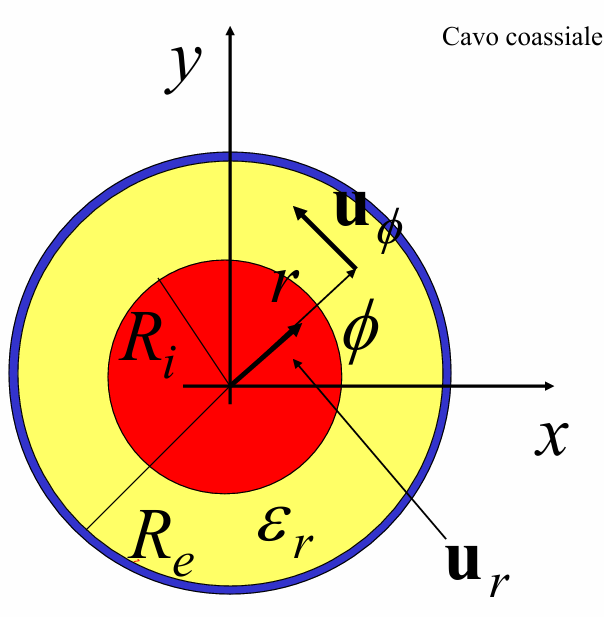
\includegraphics[scale = 0.5]{Cavo coax schematizzato.PNG}
\end{figure} 

\footnote{Slide del prof | PPT: Lezione 16 Mezzi trasmissivi 03 Maggio 23 | Pag 5} 

Visto che il cavo coassiale è formato da due conduttori, 
rispettivamente di raggio $R_i$ per il conduttore interno e di raggio $R_e$ per il conduttore esterno, 
divisi da un dielettrico, proprio come il condensatore, possiamo esprimere una carica per unità di lunghezza: 

{\Large \begin{equation}
    \begin{split}
        \hat{\rho_l} 
        &= \varepsilon \vec{E_r} (R_e, z) \hat{u_r} \cdot 2 \pi R_e \hat{u_r} \\ 
        &= \varepsilon \frac{1}{R_e \ln \left|\frac{R_e}{R_i}\right|} \vec{V} (z) \hat{u_r}  \cdot 2 \pi R_e \hat{u_r}
    \end{split}
\end{equation}}

dove l'unità di misura di $\hat{\rho_l}$ è: 

{\Large \begin{equation}
    [\hat{\rho_l} ] = \frac{C}{m}   
\end{equation}}

Proprio come il condensatore, possiamo esprimere la capacità per unità di lunghrzza come: 

{\Large \begin{equation}
    C = \frac{\hat{P_l}}{\hat{V} (z)} = \frac{2 \pi \varepsilon}{\ln \left|\frac{R_e}{R_i}\right|}
\end{equation}}

dove l'unità di misura di C è: 

{\Large \begin{equation}
    [C] = \frac{F}{m} 
\end{equation}} 

Essendo il cavo composto da due conduttori, possiamo esprimere il flusso di campo magnetico come: 

{\Large \begin{equation}
    \begin{split}
        \Phi_B 
        &= \mu_o \int_{R_i}^{R_e} \hat{H_\phi} dr \\  
        &= \mu_o \int_{R_i}^{R_e} \frac{\hat{I} (z)}{2 \pi} dr \\
        &= \mu_o \frac{\hat{I} (z)}{2 \pi} \ln \left|\frac{R_e}{R_i}\right| 
    \end{split}
\end{equation}} 

Quindi, possiamo esprimere l'induttanza per unità di lunghezza come: 

{\Large \begin{equation}
    L = \frac{\phi_B}{\hat{I}(z)} = \frac{\mu_o \ln \left|\frac{R_e}{R_i}\right|}{2 \pi}
\end{equation}}


Grazie ai valori di L e C, possiamo esprimere la velocità v, la costante di propagazione k e l'impedenza caratteristica $Z_o$: 

{\Large \begin{equation}
        Z_o = \sqrt{\frac{L}{C}} = \sqrt{\frac{\mu_o}{\varepsilon}} \frac{\ln \left|\frac{R_e}{R_i}\right| }{2 \pi} 
\end{equation}}

{\Large \begin{equation}
    v = \frac{1}{\sqrt{L C}} = \sqrt{\frac{2 \pi}{\mu_o \ln \left|\frac{R_e}{R_i}\right| } \cdot \frac{\ln \left|\frac{R_e}{R_i}\right|}{2 \pi \varepsilon}} = \frac{1}{\sqrt{\mu_o \varepsilon}}
\end{equation}} 

{\Large \begin{equation}
    \kappa = \omega \sqrt{L C} = \omega \sqrt{\mu_o \varepsilon}
\end{equation}}

\newpage 

\section{Teorema di Poynting in un cavo coax} 

\footnote{Slide del prof | PPT: Lezione 16 Mezzi trasmissivi 03 Maggio 23 | Pag 34-35}

Il teorema di Poynting è valido anche in un cavo coassiale. \\ 
Quindi, definiamo una superficie S ortogonale a $\hat{z}$: 

{\Large \begin{equation}
    \begin{split}
        \vec{S} 
        &= \vec{E} \times \vec{H}^{*} \\ 
        &= \frac{\hat{r} V(z)}{r \ln \left|\frac{R_e}{R_i}\right|}  \times \frac{\hat{\phi}}{2 \pi r} I^{*} (z) \\ 
        &= \frac{\hat{z}}{2 \pi r^{2} \cdot \ln \left|\frac{R_e}{R_i}\right|} V(z) I^{*} (z) 
    \end{split}
\end{equation}}

Dato S, possiamo calcolarci la potenza attiva trasportata da un'onda TEM in un cavo coax: 

{\Large \begin{equation}
    \begin{split}
        P &= \frac{1}{2} \Re{\int \int \vec{S} \cdot \hat{z} ds} \\ 
        &= \frac{1}{2} \Re{\int_{0}^{2 \pi} \int_{R_i}^{R_e} \vec{S} \cdot \hat{z} r dr d\phi} \\
        &= \frac{1}{2} \Re{V(z) I^{*} (z)} \\ 
        &= \frac{1}{2 Z_o} (\left|V^{+}\right| ^{2} - \left|V^{-}\right| ^{2})
    \end{split}
\end{equation}}

\newpage 

\section{Perdite nel dielettrico} 

\footnote{Slide del prof | PPT: Lezione 20 Perdite nel dieletrico 17 maggio 23 | Pag 3-4}

I due conduttori che costituiscono un cavo coax sono tenuti da un dielettrico con bassa permeattività 
(ad esempio il telflon). \\ 

\begin{tcolorbox}
Da \url{https://it.wikipedia.org/wiki/Permittivit%C3%A0_elettrica} \\
La permittività elettrica è una grandezza fisica che quantifica la tendenza del materiale a contrastare l'intensità del campo elettrico presente al suo interno. Descrive quindi il comportamento di un materiale in presenza di un campo elettrico. Viene anche comunemente chiamata costante dielettrica. \\ \\ 
La permittività elettrica è fortemente legata alla suscettività elettrica, ovvero alla predisposizione del materiale a polarizzarsi quando viene applicato un campo elettrico. La polarizzazione di atomi e molecole produce un campo elettrico aggiuntivo nel materiale, descritto attraverso il vettore induzione elettrica, e la permittività elettrica ne quantifica l'entità per unità di carica elettrica.    
\end{tcolorbox}

Quindi, il campo elettrico tra questi due conduttori è: 

{\Large \begin{equation}
    \vec{D} = \varepsilon_o \vec{E} + \vec{P_l}
\end{equation}}
 
dove $\vec{P_l}$ è la perdita del campo elettrico nel dielettrico. \\ \\ 

Se il mezzo è lineare: 

{\Large \begin{equation}
    \vec{P_l} = \varepsilon_o \chi_e \vec{E}
\end{equation}} 

\begin{tcolorbox}
    $\chi$ lettera greca che si legge chi
\end{tcolorbox}

dove $\chi_e$ tiene conto dell'energia EM dissipata sotto forma di calore. \\ \\ 

Permeattività complessa: 

{\Large \begin{equation}
    \begin{split}
        \varepsilon 
        &= \varepsilon_o (1 + \chi_e) \\ 
        &= \varepsilon_o \varepsilon_r (1 - \jmath \tan \delta)
    \end{split}
\end{equation}}

\begin{tcolorbox}
    $\delta$ lettera greca che si legge delta
\end{tcolorbox}

dove: 

$\delta$ è un parametro del dielettrico e non dipende dalla profondità di penetrazione. 

\begin{tcolorbox}
    Da \url{https://www.scienzaatscuola.it/fisica%205g/vivente3.html} \\ 
    La quantità $\delta$ è detta profondità di penetrazione e indica la distanza alla quale i campi si sono ridotti a circa il 37\% e la densità di potenza si è ridotta a meno del 14\% rispetto ai valori all'interfaccia. 
\end{tcolorbox}

Sapendo $\delta$, possiamo esprimere $\kappa$ come: 

{\Large \begin{equation}
    \begin{split}
        \kappa 
        &= \omega \sqrt{\mu_o \varepsilon} \\ 
        &\approx \omega \sqrt{\mu_o \varepsilon_o \varepsilon_r } (1 - \jmath \frac{\tan \delta}{2})    
    \end{split}
\end{equation}}

Inoltre, possiamo esprimere una costante di attenuazione del dielettrico $\alpha_d$ come: 

{\Large \begin{equation}
    \alpha_d \approx \kappa \frac{\tan \delta}{2}
\end{equation}}

Oltre al dielettrico, il cavo coax presente due conduttori, quindi possiamo 
esprimere una costante di attenuazione del conduttore $\alpha_c$ come: 

{\Large \begin{equation}
    \begin{split}
        \alpha_c 
        &= \frac{P_l (z)}{2P(z)} \\ 
        &\approx \frac{\frac{R_s}{4 \pi} [\frac{1}{R_i} + \frac{1}{R_e}]}{Z_o} \\ 
        &= \frac{\frac{R_s}{4 \pi R_i} [1 + \frac{R_i}{R_e}]}{\frac{\eta}{2 \pi} \ln \left|\frac{R_e}{R_i}\right|}
    \end{split}
\end{equation}} 

dove: 

{\Large \begin{equation}
    \begin{cases}
        R_s = \frac{1}{\sigma \delta} \\ 
        \delta = \frac{1}{\sqrt{\pi f \mu_o \sigma}}
    \end{cases}
\end{equation}}

\begin{tcolorbox}
    $\delta$ lettera greca si legge delta
\end{tcolorbox}

Spesso, è preferibile esprimere le perdite totali in un cavo coax in dB: 

{\Large \begin{equation}
    \alpha_{dB} = -20 \log e^{- (\alpha_c + \alpha_d)}
\end{equation}} 

\newpage 

\section{Perdite dipendenti dalla temperatura nel dielettrico}

\footnote{Slide del prof | PPT: Lezione 20 Perdite nel dieletrico 17 maggio 23 | Pag 15}

La temperatura influisce sul coefficiente elettrico di attenuazione $\alpha(T)$: 

{\Large \begin{equation}
    \alpha (T) = \alpha_{293 K} \cdot \sqrt{1 + \sigma_P (\frac{T}{K} - 293)}
\end{equation}}


dove: 
\begin{itemize}
    \item $\alpha_P$ è il coefficiente di resistività (è un parametro empirico riguardo al materiale del conduttore) 
    \item $\alpha_{293 K}$  è la resistività a 293 Kelvin 
\end{itemize}

Se il cavo coax è corto circuitato: 

{\Large \begin{equation}
    V^{+} = -V^{-}
\end{equation}} 

Quindi: 

{\Large \begin{equation}
    V_{max} = 2 \left|V^{+}\right|
\end{equation}}

\newpage 

\chapter{Guide d'onda} 

\begin{figure}[h]
    \centering
    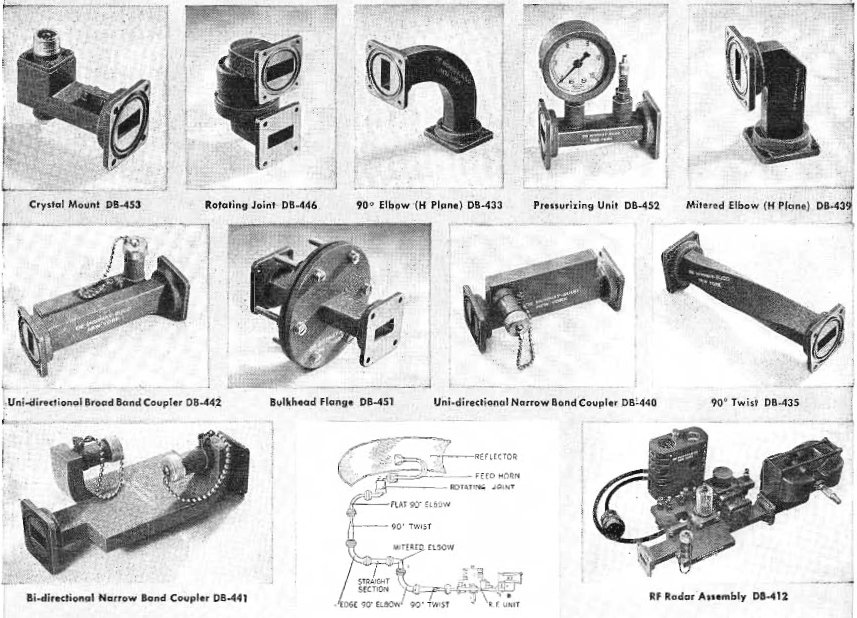
\includegraphics[scale = 0.5]{Waveguide_collection.jpg}
\end{figure} 

\newpage 

\section{Cosa sono le guide d'onda} 

\footnote{FWC - pag 395 \\ 8.1 Introduction}

La guida d'onda è una struttura, o parte di una struttura, che permette 
ad un'onda di propagarsi in una precisa direzione. \\ 

Se la guida d'onda cambia direzione, l'onda è costretta a seguirla. \\ 

I componenti trasversali dell'onda si propagheranno lungo la direzione di propagazione. \\ 

Generalmente, nelle analisi delle guide d'onda, siamo interessati alla distribuzione dei campi EM; 
ma, la cosa più importante è la dipendenza della costante di propagazione rispetto alla frequenza. \\ 

Dalla costante di propagazione è possibile calcolare la velocità dell'onda, 
la variazione di fase e l'attenuazione lungo la guida d'onda. \\ 

\newpage 

\section{Equazioni delle guide d'onda per sistemi uniformi} 
\footnote{FWC - pag 396 \\ 8.2 Basic equations and wave types for uniform systems}

Nelle guide d'onda considereremo onde del tipo: 

{\Large 
    \begin{equation}
        e^{\jmath \omega t - \gamma z}
    \end{equation}
}

quindi onde a tempo armonico $\jmath \omega t$ e che variano con la distanza $ - \gamma z$. \\ \\ 


\begin{tcolorbox}
    $\gamma$ dall'alfabeto greco si legge gamma 
\end{tcolorbox}


La costante di propagazione $\gamma$ sarà importante per le proprietà dell'onda, 
come ad esempio di quanto si attenua l'onda, la fase e la velocità di gruppo. \\ \\ 

Assumiamo nessuna densità di carica in ingresso e considereremo i conduttori della guida d'onda soddisfino l'equazione: 

{
    \Large
    \begin{equation}
        \kappa^{2} = \omega^{2} \mu \varepsilon
    \end{equation}
} 

Le equazioni dell'onda, che si riducono alle equazioni di Helmholtz per i campi fasoriali, saranno: 

{
    \Large 
    \begin{equation}
        \begin{cases}
            \nabla ^{2} \vec{E} = - \kappa ^{2}  \vec{E} \\ 
            \nabla ^{2} \vec{H} = - \kappa ^{2}  \vec{H} \\    
        \end{cases}
    \end{equation}
}

Nelle coordinate cartesiane, $\nabla ^{2}$, chiamato anche operatore di Laplace, può essere suddiviso in due parti: 

{
    \Large 
    \begin{equation}
        \begin{split}
            \nabla ^{2} \vec{E} 
            &= \frac{\partial ^{2} \vec{E}}{\partial x ^{2}} + \frac{\partial ^{2} \vec{E}}{\partial y ^{2}} + \frac{\partial ^{2} \vec{E}}{\partial z ^{2}}
            \\
            &= \nabla_t ^{2} \vec{E} + \frac{\partial ^{2} \vec{E}}{\partial z^{2}}  
        \end{split}
    \end{equation}
} 

dove, $\nabla_t ^{2}$ lo definiamo come operatore di Laplace trasversale. \newline 

Assumendo la funzione di propagazione lungo l'asse x $e^{-\gamma z}$, possiamo scrivere: 

{
    \Large
    \begin{equation} 
        \frac{\partial ^{2} \vec{E}}{\partial z^{2}} = \gamma ^{2} \vec{E}
    \end{equation}
}

Uguagliando i due modi di esprimere $\nabla ^{2} \vec{E}$ e sostituendo il 
valore di $ \frac{\partial ^{2} \vec{E}}{\partial z^{2}}$, possiamo scrivere la seguente equazione: 

{
    \Large 
    \begin{equation}
        \begin{cases}
            \nabla ^{2} \vec{E} = - \kappa ^{2}  \vec{E} \\
            \nabla ^{2} \vec{E} = \nabla_t ^{2} \vec{E} + \frac{\partial ^{2} \vec{E}}{\partial z^{2}}
        \end{cases} 
        \Rightarrow
        - \kappa ^{2}  \vec{E} = \nabla_t ^{2} \vec{E} + \gamma ^{2} \vec{E}
    \end{equation}
}

Oppure, svolgendo diversi passi algebrici: 

{
    \Large
    \begin{equation}
        \begin{split}
            \nabla_t ^{2} \vec{E} 
            &= - \kappa ^{2}  \vec{E} - \gamma ^{2}  \vec{E} \\ 
            &= -(\kappa ^{2} + \gamma ^{2}) \vec{E} 
        \end{split}
    \end{equation}
}

I passaggi algebrici svolti per $\nabla_t ^{2} \vec{E}$ possono essere svolti 
anche per $\nabla_t ^{2} \vec{H}$: 

{
    \Large
    \begin{equation}
        \nabla_t ^{2} \vec{H} = -(\kappa ^{2} + \gamma ^{2}) \vec{H}
    \end{equation}
}

$\nabla_t ^{2} \vec{E}$ e $\nabla_t ^{2} \vec{H}$ sono equazioni differenziali che devono essere soddisfatte 
nelle regione del dielettrico della linea di trasmissione o della guida d'onda. \\ 


La procedura standard è quella di trovare i componenti di $\vec{E}$ e $\vec{H}$ lungo 
l'asse z che soddisfano $\nabla_t ^{2} \vec{E}$ e $\nabla_t ^{2} \vec{H}$, quindi le condizioni al contorno, oppure 
esplicitato in una maniera differente, troviamo $E_z$ e $H_z$ in modo tale che siano le variabili indipendenti del sistema. \\ 

Consideriamo le equazioni di $e^{\jmath \omega t - \gamma z}$ 
in forma fasoriale divise nei loro componenti. \\ 

Dalle leggi di Maxwell avremo: 

{
    \Large 
    \begin{equation}
            \nabla \times \vec{E} 
            = \operatorname{rot}
            \begin{vmatrix}
                \hat{x} & \hat{y} &\hat{z} \\ \\ 
                \frac{\partial}{\partial x} & \frac{\partial}{\partial y} & -\gamma \\ \\ 
                E_x & E_y & E_z
            \end{vmatrix}  
    \end{equation}
}

Svolgendo diversi passi algebrici: 

{
    \Large 
    \begin{equation}
        \nabla \times \vec{E} 
            = 
            \hat{x} 
            \begin{vmatrix}
            \frac{\partial}{\partial y} & -\gamma \\  \\ 
            E_y & E_z 
            \end{vmatrix}
            -\hat{y} 
            \begin{vmatrix}
            \frac{\partial}{\partial x} & -\gamma \\  \\ 
            E_x & E_z 
            \end{vmatrix}
            +\hat{z} 
            \begin{vmatrix}
            \frac{\partial}{\partial x} & \frac{\partial}{\partial y} \\  \\ 
            E_x & E_y 
            \end{vmatrix}
    \end{equation}
}

{
    \Large 
    \begin{equation}
            \nabla \times \vec{E}
            = 
            \hat{x} 
            [
                \frac{\partial E_z}{\partial y} 
                +\gamma E_y
            ]    
            -\hat{y} 
            [
                \frac{\partial E_z}{\partial x} 
                +\gamma E_x
            ]    
            +\hat{z} 
            [
                \frac{\partial E_y}{\partial x} 
                + \frac{\partial E_x}{\partial y}
            ] 
    \end{equation}
}

{
    \Large 
    \begin{equation}
            \nabla \times \vec{E}
            =        
\hat{x} 
[
    \frac{\partial E_z}{\partial y} 
    +\gamma E_y
]    
+\hat{y} 
[
    -\frac{\partial E_z}{\partial x} 
    -\gamma E_x
]    
+\hat{z} 
[
    \frac{\partial E_y}{\partial x} 
    + \frac{\partial E_x}{\partial y}
] 
    \end{equation}
}       


Dalle equazioni di Maxwell in forma fasoriale: 

{
    \Large 
    \begin{equation}
        \nabla \times \vec{E} = -\jmath \omega \mu \vec{H}
    \end{equation}
}

Divendendo questa equazione nei vari assi cartesiani: \\ 

\textbf{Asse X} 

{
    \Large 
    \begin{equation}
        \frac{\partial E_z}{\partial y} + \gamma E_y 
        = 
        -\jmath \omega \mu H_x
    \end{equation}
}


\textbf{Asse Y} 

{
    \Large 
    \begin{equation}
        - \gamma E_x - \frac{\partial E_z}{\partial x}  
        = 
        -\jmath \omega \mu H_y
    \end{equation}
}



\textbf{Asse Z} 

{
    \Large 
    \begin{equation}
        \frac{\partial E_y}{\partial x} - \frac{\partial E_x}{\partial y} 
        = 
        -\jmath \omega \mu H_z
    \end{equation}
}

Sostituendo $\vec{H}$ ad $\vec{E}$, possiamo trovare le equazioni 
di Maxwell in forma fasoriale di: 

Dalle equazioni di Maxwell in forma fasoriale: 

{
    \Large 
    \begin{equation}
        \nabla \times \vec{H} = \jmath \omega \varepsilon \vec{E}
    \end{equation}
}


\textbf{Asse X} 

{
    \Large 
    \begin{equation}
        \frac{\partial H_z}{\partial y} + \gamma H_y 
        = 
        \jmath \omega \varepsilon E_x
    \end{equation}
}


\textbf{Asse Y} 

{
    \Large 
    \begin{equation}
        - \gamma H_x - \frac{\partial H_z}{\partial x}  
        = 
        \jmath \omega \varepsilon E_y
    \end{equation}
}



\textbf{Asse Z} 

{
    \Large 
    \begin{equation}
        \frac{\partial H_y}{\partial x} - \frac{\partial H_x}{\partial y} 
        = 
        \jmath \omega \varepsilon E_z
    \end{equation}
}

Ora è possibile trovare $E_x$, $E_y$, $H_x$, $H_y$ 
in funzione di $E_z$ e $H_z$. \\ 

I passaggi algebrici sono omessi, però basta sostituire i valori. \\ 

Alla fine troveremo i i valori di: 

{
    \Large 
    \begin{equation}
        \begin{cases}
            E_x = - \frac{1}{\gamma ^{2} + \kappa ^{2}} (\gamma \frac{\partial E_z}{\partial x} + \jmath \omega \mu \frac{\partial H_z}{\partial y}) \\ \\ 
            E_y =  \frac{1}{\gamma ^{2} + \kappa ^{2}} (- \gamma \frac{\partial E_z}{\partial y} + \jmath \omega \mu \frac{\partial H_z}{\partial x}) \\ \\ 
            H_x =  \frac{1}{\gamma ^{2} + \kappa ^{2}} (- \gamma \frac{\partial H_z}{\partial x} + \jmath \omega \varepsilon \frac{\partial E_z}{\partial y}) \\ \\ 
            H_y =  -\frac{1}{\gamma ^{2} + \kappa ^{2}} ( \gamma \frac{\partial H_z}{\partial y} + \jmath \omega \varepsilon \frac{\partial E_z}{\partial x}) 
        \end{cases}
    \end{equation}
}

È conveniente scrivere: 

{
    \Large
    \begin{equation}
        \begin{cases}
            \gamma = \jmath \beta \\ 
            \kappa_c ^{2} = \gamma^{2} + \kappa^{2} = \kappa^{2} - \beta^{2} 
        \end{cases}
    \end{equation}
}



Le equazioni precedentemente scritte, diventeranno: 

{
    \Large 
    \begin{equation}
        \begin{cases}
            E_x = - \frac{\jmath}{\kappa_c ^{2}} (\beta \frac{\partial E_z}{\partial x} + \omega \mu \frac{\partial H_z}{\partial y}) \\ \\ 
            E_y =  \frac{\jmath}{\kappa_c ^{2}} (- \beta \frac{\partial E_z}{\partial y} + \omega \mu \frac{\partial H_z}{\partial x}) \\ \\ 
            H_x =  \frac{\jmath}{\kappa_c ^{2}} (- \beta \frac{\partial H_z}{\partial x} + \omega \varepsilon \frac{\partial E_z}{\partial y}) \\ \\ 
            H_y =  -\frac{\jmath}{\kappa_c ^{2}} ( \beta \frac{\partial H_z}{\partial y} + \omega \varepsilon \frac{\partial E_z}{\partial x}) 
        \end{cases}
    \end{equation}
}

Inoltre possiamo scrivere: 

{
    \Large 
    \begin{equation}
        \begin{cases}
            \nabla_t ^{2} E_z = - \kappa_c ^{2} E_z \\ \\
            \nabla_t ^{2} H_z = - \kappa_c ^{2} H_z     
        \end{cases}
    \end{equation} 
}

\newpage
\chapter{Guide d'onda rettangolari} 

\begin{figure}[h]
    \centering
    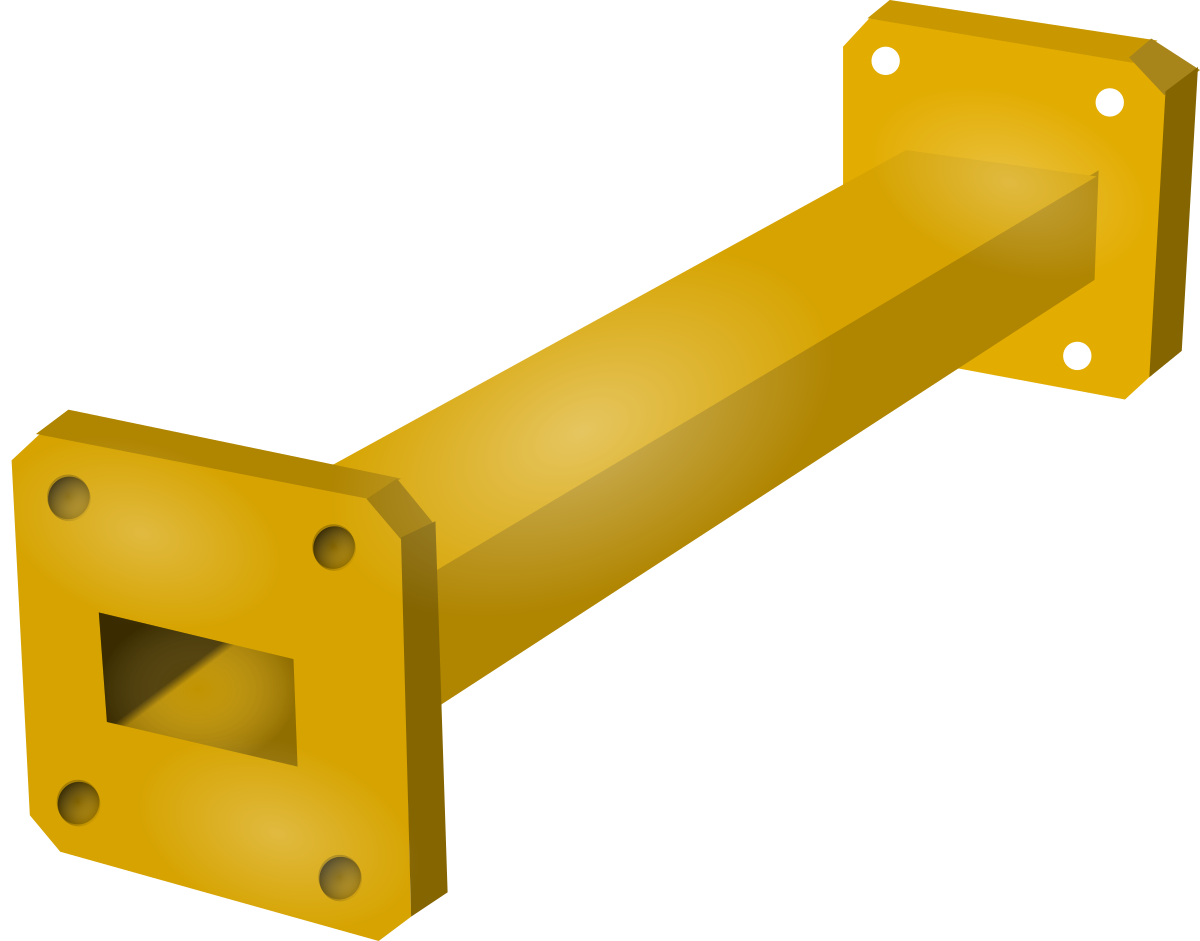
\includegraphics[scale = 0.35]{Waveguide17-with-UBR120-flanges-svg.svg.png}
\end{figure} 

\newpage 

\section{Cosa sono le guide d'onda rettangolari} 

\footnote{FWC - pag 417 \\ 8.7 Rectangular waveguides}

\begin{figure}[h]
    \centering
    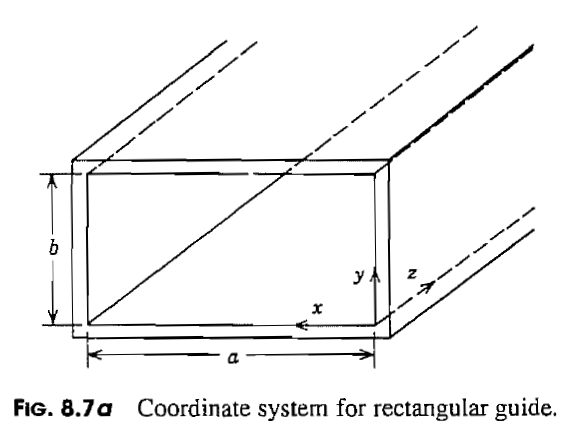
\includegraphics{Coordinate system for rectangular guide.PNG}
\end{figure} 

Le onde rettangolari sono un tipo d'onda in cui la sezione è formata da una regione dielettrica di larghezza 
a e di altezza b che si estende per una lunghezza infinita lungo la direzione z, 
regione dielettrica rivestita da quattro conduttori. \\ 

Non ci possono essere onde TEM perchè la componente lungo z non varia (considerando che nella guida d'onda possono 
esistere onde del tipo $e^{-\jmath \omega t - \gamma z}$ e che quindi variano di $\gamma$ lungo l'asse z). \\ 

Onde TM e TE possono esistere in una guida d'onda rettangolare. 

\newpage 

\section{Onde TM nelle guide d'onda rettangolari} 

\footnote{FWC - pag 418 \\ 8.7 Rectangular waveguides - TM Waves} 

Le onde TM, lungo la componente dell'asse z: 

{
    \Large 
    \begin{equation}
        \begin{cases}
            H_z = 0 \\ 
            E_z \neq 0
        \end{cases}
    \end{equation}
}

Dalle equazioni di Maxwell per le guide d'onda, abbiamo trovato che: 

{
    \Large 
    \begin{equation}
        \nabla_t ^{2} E_z 
        = \frac{\partial ^{2} E_z}{\partial x^{2}} + \frac{\partial ^{2} E_z}{\partial y^{2}}
        = - \kappa_c ^{2} E_z
    \end{equation}
}

dove: 

{
    \Large 
    \begin{equation}
        \kappa_c ^{2} = \kappa_x ^{2} + \kappa_y ^{2}
    \end{equation}
}

Quindi: 

{
    \Large 
    \begin{equation}
        \frac{\partial ^{2} E_z}{\partial x^{2}} + \frac{\partial ^{2} E_z}{\partial y^{2}}
        = - \kappa_c ^{2} E_z
        \Rightarrow 
        \frac{\partial ^{2} E_z}{\partial x^{2}} + \frac{\partial ^{2} E_z}{\partial y^{2}}
        =  - \kappa_x ^{2} - \kappa_y ^{2} E_z
    \end{equation}
}

Utilizzando la separazione delle variabili (x,y) possiamo portare questa 
equazione in un sistema per ogni variabile, cioè: 

{
    \Large
    \begin{equation}
        \begin{cases}
            \frac{\partial ^{2} E_z}{\partial x^{2}} 
            = - \kappa_x ^{2} E_z \\ \\
            \frac{\partial ^{2} E_z}{\partial y^{2}} 
            = - \kappa_y ^{2} E_z  
        \end{cases}
    \end{equation}
}


Il cui risultato è rispettivamente \\ 
per l'asse x: 

{
    \Large 
    \begin{equation}
        A^{'} \sin(\kappa_x x) + B^{'} \cos(\kappa_x x) 
    \end{equation}
}

per l'asse y: 

{
    \Large 
    \begin{equation}
        C^{'} \sin(\kappa_y y) + D^{'} \cos(\kappa_y y) 
    \end{equation}
}

dove $A^{'}$, $B^{'}$, $C^{'}$, $D^{'}$ sono coefficienti reali. \\ 

La separazione delle variabili ci impone di moltiplicare i risultati 
per l'asse x e l'asse y, quindi $E_z$ diventa: 

{
    \Large 
    \begin{equation}
        E_z 
        = 
        (A^{'} \sin(\kappa_x x) + B^{'} \cos(\kappa_x x))  (C^{'} \sin(\kappa_y y) + D^{'} \cos(\kappa_y y))
    \end{equation}
}

Siccome consideriamo le pareti della guida d'onda come perfetti conduttori, 
$E_z = 0$ in: 

{
    \Large 
    \begin{equation}
        \begin{cases}
            x = 0 \\ 
            y= 0
        \end{cases}
    \end{equation}
} 

Allora: 

{
    \Large 
    \begin{equation}
        \begin{cases}
            B^{'}= 0 \\ 
            D^{'}= 0
        \end{cases}
    \end{equation}
} 

Ponendo: 

{
    \Large 
    \begin{equation}
            A^{'}C^{'} = A 
    \end{equation}
} 

e considerando le semplificazioni svolti, $E_z$ diventerà: 

{
    \Large 
    \begin{equation}
        E_z = A \sin(\kappa_x x) \sin(k_y y)
    \end{equation}
}

Per $A \neq 0$, $E_z = 0$ non solo in (0, 0), ma anche in: 

{
    \Large 
    \begin{equation}
        \begin{cases}
            x = a \\ 
            y= b
        \end{cases}
    \end{equation}
}

Essendo il $\sin$ una funzione sinusoidale, possiamo scrivere che
$E_z = 0$ non solo per in (a, b) ma anche in: 

{
    \Large
    \begin{equation}
        \begin{cases}
            \sin(\kappa_x x) = 0 
            \Rightarrow 
            \kappa a = m \pi \\ 
            \sin(\kappa_y y) = 0 
            \Rightarrow 
            \kappa b = n \pi 
        \end{cases}
    \end{equation}
}

dove m e n è un numero intero maggiore di 0. \\ 

Quindi per un'onda $TM_{n m}$, la frequanza di cut-off, cioè 
la frequenza per cui $E_z = 0$ è: 


{
    \Large 
    \begin{equation}
        \begin{split}
            \omega_{c_{m,n}} 
            &= 
            \frac{\kappa_{c_{m,n}}}{\sqrt{\mu \varepsilon}} \\
            &= 
            \frac{1}{\sqrt{\mu \varepsilon}} \sqrt{[(\frac{n \pi}{a}) ^{2} + (\frac{m \pi}{b}) ^{2}]}    
        \end{split}
    \end{equation}
}

Siccome sappiamo che: 

{
    \Large 
    \begin{equation}
        \kappa_c ^{2} = \kappa^{2} - \beta^{2}
    \end{equation}
}

è possibile trovare la costante di fase per le frequenze 

{
    \Large 
    \begin{equation}
        \begin{cases}
            \alpha 
            = 
            \kappa_{c_{m,n}} \sqrt{1 - (\frac{\omega}{\omega_{c_{m,n}}})} 
            \text{  per } 
            \omega < \omega_{c_{m,n}}
            \\ \\
            \beta
            = 
            \kappa \sqrt{1 - (\frac{\omega_{c_{m,n}}}{\omega})} 
            \text{  per } 
            \omega > \omega_{c_{m,n}}
        \end{cases}
    \end{equation}
}

La velocità di fase di gruppo sono rispettivamente: 

{
    \Large
    \begin{equation}
        \begin{cases}
            v_p 
            = 
            \frac{\omega}{\beta} 
            = 
            \frac{v}{\sqrt{1 - (\frac{\omega_{c_{m,n}}}{\omega})}}
            \\ \\
            v_g 
            = 
            \frac{ d \omega}{ d \beta} 
            = 
            v\sqrt{1 - (\frac{\omega_{c_{m,n}}}{\omega})}
        \end{cases}
    \end{equation}
}

\begin{tcolorbox}
    In fisica la velocità di fase è la velocità con cui si propaga la fase di un'onda, sia essa elettromagnetica o meccanica. La velocità di fase può essere visualizzata come la velocità di propagazione di una cresta dell'onda ma non coincide necessariamente con la velocità di propagazione di un segnale (che è più propriamente descritta dalla velocità di gruppo) e quindi può essere più alta della velocità della luce senza violare la relatività ristretta. \\
    \url{https://it.wikipedia.org/wiki/Velocit%C3%A0_di_fase} \\ \\
    La velocità di gruppo di un'onda è la velocità con cui si propagano nello spazio le variazioni nella forma dell'ampiezza dell'onda. \\
    La velocità di gruppo è spesso considerata la velocità a cui l'energia o l'informazione sono trasportate dall'onda. In molti casi questa è una visione accurata, e la velocità di gruppo può essere pensata come la velocità di segnale della forma d'onda. \\
    \url{https://it.wikipedia.org/wiki/Velocit%C3%A0_di_gruppo}
\end{tcolorbox}

\newpage 

\section{Onde TE nelle guide d'onda rettangolari} 

\footnote{FWC - pag 419 \\ 8.7 Rectangular waveguides - TE Waves}

Il procedimento sarà simile al caso precedente delle onde TM, ma cambieranno alcune cose. \\ 

Prima di tutto, nelle onde TE abbiamo che: 

{
    \Large 
    \begin{equation}
        \begin{cases}
            H_z \neq 0 \\ 
            E_z = 0
        \end{cases}
    \end{equation}
}

Inoltre: 
{
    \Large 
    \begin{equation}
        \nabla_t ^{2} H_z 
        = \frac{\partial ^{2} H_z}{\partial x^{2}} + \frac{\partial ^{2} H_z}{\partial y^{2}}
        = - \kappa_c ^{2} H_z
    \end{equation}
}

Facendo lo stesso procedimento della separazione delle variabili del caso TE, abbiamo che: 

{
    \Large 
    \begin{equation}
        H_z 
        = 
        (A^{'} \sin(\kappa_x x) + B^{'} \cos(\kappa_x x)) (C^{'} \sin(\kappa_y y) + D^{'} \cos(\kappa_y y))
    \end{equation}
}

I vari componenti dell'onda saranno: 

{
    \Large
    \begin{equation}
        \begin{split}
            E_x 
            &= 
            -\frac{\jmath \omega \mu}{\kappa_c ^{2}} \frac{\partial H_z}{\partial y}
            \\ \\ \\
            &= 
            - \frac{\jmath \omega \mu \kappa_y}{\kappa_c ^{2}} (A^{'} \sin(\kappa_x x) + B^{'} \cos(\kappa_x x)) (C^{'} \cos(\kappa_y y) - D^{'} \sin(\kappa_y y))
        \end{split}
    \end{equation}
}

{
    \Large
    \begin{equation}
        \begin{split}
            E_y 
            &= 
            \frac{\jmath \omega \mu}{\kappa_c ^{2}} \frac{\partial H_z}{\partial x}
            \\ \\ \\
            &= 
            \frac{\jmath \omega \mu \kappa_x}{\kappa_c ^{2}} (A^{'} \cos(\kappa_x x) - B^{'} \sin(\kappa_x x)) (C^{'} \sin(\kappa_y y) + D^{'} \cos(\kappa_y y))
        \end{split}
    \end{equation}
}

In questo caso, però: 

{
    \Large
    \begin{equation}
        \begin{cases}
            E_x = 0 \text{  per } (x, 0) \Rightarrow C^{'} = 0 \\ 
            E_x = 0 \text{  per } (0, y) \Rightarrow A^{'} = 0 \\ 
        \end{cases}
    \end{equation}
}

Ponendo: 

{
    \Large 
    \begin{equation}
        B = B^{'}D^{'}
    \end{equation}
}

$H_z$ diventa: 

{
    \Large 
    \begin{equation}
        H_z = B \cos(\kappa_x x)\cos(\kappa_y y)
    \end{equation}
}

Per $E_x = 0$ in $y=b$ ,quindi: 

{
    \Large
    \begin{equation}
        \kappa_y b = n \pi
    \end{equation}
}

Per $E_y = 0$ in $x=a$ ,quindi: 

{
    \Large
    \begin{equation}
        \kappa_x a = m \pi
    \end{equation}
}

A differenza delle onde TM, basta solo che sia soddisfatta 
solo una delle due condizioni elencate precedentemente per avere continuità 
dell'onda. \\ 

$\omega_{c_{m,n}}$, $\alpha$, $\beta$, $v_p$ e $v_g$ sono le stesse della $TM_{n, m}$ 

\newpage 
 
\chapter{Modi di guida d'onda rettangolare} 

\begin{figure}[h]
    \centering
    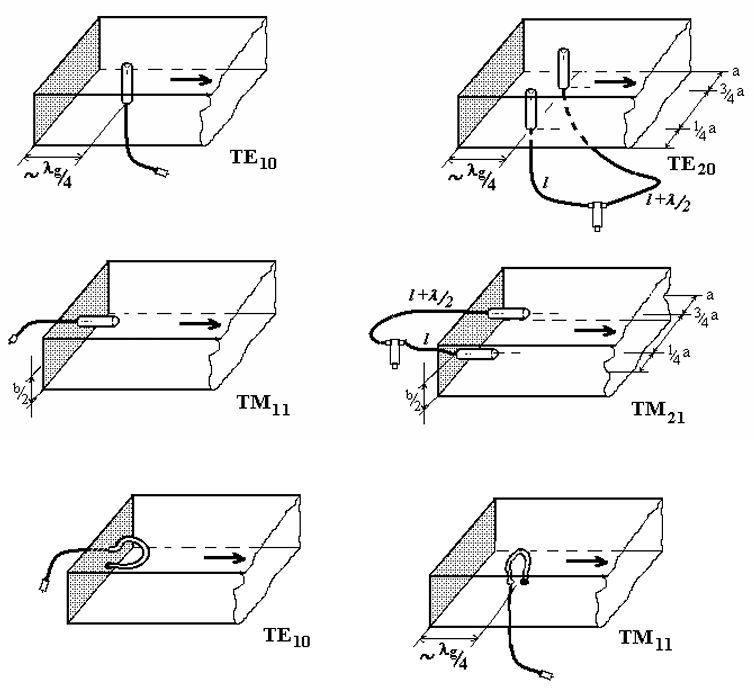
\includegraphics[scale = 0.9]{Modi di guida rettangolare.PNG}
\end{figure}  

\newpage 

\section{Modo fondamentale: $TE_{10}$}

\footnote{Slide del prof | PPT: Lezione 21 - 22 Guide rettangolari 22-24 maggio 2023 | Pag 13-20 \\ 
FWC - pag 422 \\
FWC - 8.8 The $TE_{10}$ wave in a rectangular guide - pag 423 \\
Ricevimento con prof}

\begin{tcolorbox}
    $TE_{10}$ si legge TE uno zero, non TE dieci, si legge cifra per cifra
\end{tcolorbox}

Le guide d'onda, come scritto precedentemente, possono essere $TM_{n, m}$ o $TE_{n, m}$ e variano in base ai parametri n e m. \\ 

$TE_{10}$, o detto anche modo fondamentale, è il modo di guida d'onda per cui la frequenza di taglio è minore rispetto alle altre modalità. \\ 

In formule: 

{
    \Large 
    \begin{equation}
        f_{c_{10}} = \frac{c}{2} \frac{1}{a} = \frac{1}{2 a \sqrt{\mu \varepsilon}}
    \end{equation} 
}

\begin{tcolorbox}
    Dal ricevimento con il prof: \\ \\ 

    Data la banda delle frequenze operative (cioè quelle che vogliamo trasmettere nel sistema guida d'onda), 
chiamata anche finestra: 

{
    \Large
    \begin{equation}
        B = [f_1, f_2]
    \end{equation}
} 

possiamo progettare le dimensioni della sezione della guida d'onda. \\ 

$f_2$ possiamo esprimerla anche come: 
{
    \Large
    \begin{equation}
        f_2 = \frac{f_2}{f_1} \cdot f_1 = k \cdot f_1
    \end{equation}
}
Se B è minore dell'intervallo di monomodalità, generalmente, 
è preferibile calcolare, dato B, la sezione di guida d'onda più grande possibile. \\

Coincidiamo l'estremo superiore della finestra con l'estremo superiore della banda di monomodalità, 
cosicchè le perdite sono più basse possibili perchè la finestra è più lontana 
possibile dalla frequenza di cut-off, ricordando più si avvicina alla frequenza di cut-off e maggiori sono le perdite. \\ 

Quindi: 

{
    \Large
    \begin{equation}
        f_2 [GHz] = \frac{300}{a [mm]} 
        \Rightarrow 
        a [mm] = \frac{300}{f_2 [GHz]} 
        = \frac{300}{k \cdot f_1 [GHz]}
    \end{equation}
}

e poi: 

{
    \Large 
    \begin{equation}
        b = \frac{1}{2} a 
    \end{equation}
}


\end{tcolorbox}

\begin{figure}[h]
    \centering
    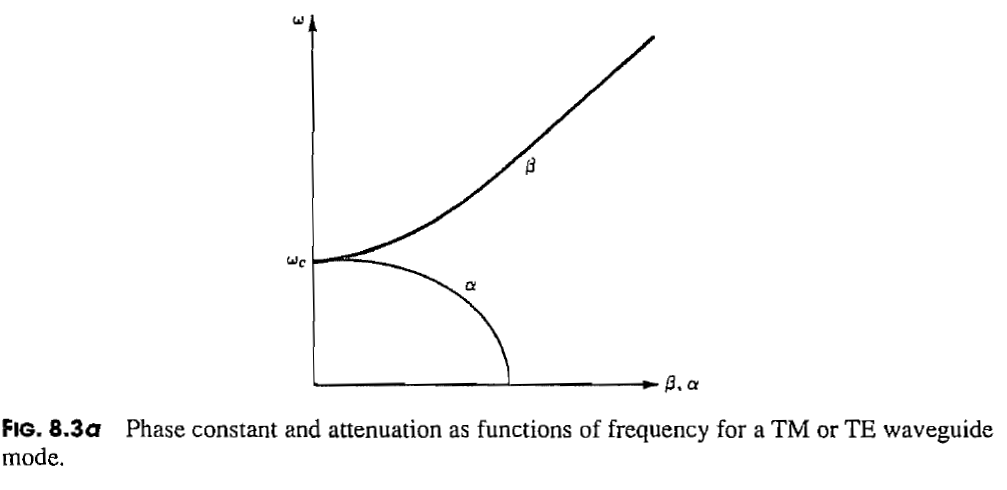
\includegraphics[scale = 0.7]{Phase constant and attenuation in parallel waveguide.PNG}
\end{figure}  

\footnote{FWE - pag 401}

\begin{tcolorbox}
    Scritto in un'altra maniera, l'onda deve essere larga almeno $\frac{\lambda}{2}$, 
    sennò non c'è propagazione. \\
    Per approfondire: \\ 
    \url{https://www.ariparma.it/risorse/articoli/Guida%20di%20onda.pdf} 
        
\end{tcolorbox}

\begin{figure}[h]
    \centering
    \includegraphics{Frequenze di cut-off in base alla modalità della guida d'onda.PNG}
\end{figure}  


La figura indica le frequenze di cut-off di diversi modi di guida d'onda. \\ 
Tipicamente, nella $TE_{10}$: 

{
    \Large
    \begin{equation}
        \frac{b}{a} = \frac{1}{2}
    \end{equation}
}

che è il valore tipicamente utilizzato nella realtà. \\ 
Normalmente, questo tipo d'onda è progettata in modo tala che la frequenza di cut-off sia il 30 per cento sotto la frequenza operativa. \\ 
In questo modo, solo un tipo d'onda si può propagare nella guida d'onda. \\ 

\begin{figure}[h]
    \centering
    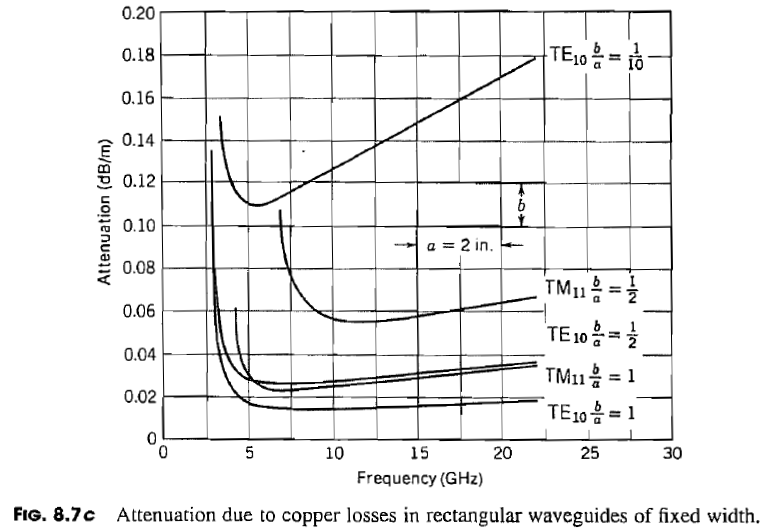
\includegraphics[scale = 0.8]{Atenuanzioni di guida d'onda con rame.PNG}
\end{figure}  



Non essendo troppo vicino alla frequenza di taglio, 
le dispersioni causate da diverse velocità di gruppo per diversi componenti di frequenze vengono minimizzati.  \\ 

Inoltre, nel modo fondamentale, la polarizzazione dei campi è fissa, 
il campo elettrico passa dal basso all'alto della guida. \\
Questa polarizzazione potrebbe essere necessaria per qualche applicazione. \\

Generalmente, viene impegato il rame come componente per le guide d'onde, e data una frequenza, l'attenuazione non è eccessivamente bassa 
rispetto a guide di altre dimensioni. \\

Nel modo fondamentale, il campo EM è il seguente: 

{
    \Large
    \begin{equation}
        \begin{cases}
            E_x = H_y = E_z = 0 \\ \\
            H_x ^{\pm} = \frac{\jmath}{\kappa_c ^{2}} \frac{\pi}{a} \beta A_{10} \sin(\frac{\pi}{a}) x e^{-\mp \jmath \beta z} \\ \\
            E_y ^{\pm} = - \frac{\jmath}{\kappa_c ^{2}} \omega \mu \frac{\pi}{a} A_{10} \sin(\frac{\pi}{a}) x e^{-\mp \jmath \beta z} 
        \end{cases}
    \end{equation}
}

in cui: 

{
    \Large 
    \begin{equation}
        \beta = \sqrt{\kappa ^{2} - (\frac{\pi}{a})^{2}}
    \end{equation}
} 

L'impedenza d'onda è uguale a: 

{
    \Large 
    \begin{equation}
        \begin{split}
            Z_{TE_{10}} 
            &= 
            - \frac{E_y}{H_x} 
            \\ 
            &= 
            \frac{\omega \mu_o}{\beta}
            \\ 
            &= 
            \frac{\omega \mu_o}{\sqrt{\kappa ^{2} - (\frac{\pi}{a})^{2}}}
        \end{split}
    \end{equation}
} 

Dal Teorema di Poynting, il flusso di potenza attiva media è:
{
    \Large
    \begin{equation}
        \begin{split}
            P_{10} 
            &= \frac{1}{2} \Re [\int_{0}^{a} \int_{0}^{b} \vec{E} \times \vec{H} ^{*} \hat{z} dx dy]
            \\ 
            &= \frac{1}{2} \Re [\int_{0}^{a} \int_{0}^{b} E_y H_x ^{*} \cdot \hat{z} dx dy]
            \\ 
            &= \frac{\omega \mu a^{3} b}{4 \pi ^{2}} \left|A_{10}\right| ^{2} \Re(\beta) 
            \\ 
            &= 
            \frac{\beta}{\omega \mu_o} \frac{\left|V^{+}\right|^{2}}{2}
        \end{split}
    \end{equation}
}


L'unico componente del campo elettrico è quello verticale $E_y$ che passa dall'alto al basso della guida. \\

$E_y$ è è massima al centro della guida e zero alle pareti della guida d'onda. \\
$H_x = 0$ alle due pareti e massimo al centro della guida, proprio come $E_y$. \\ 
$H_z$ è massima alle pareti e zero al centro. 

\begin{figure}[h]
    \centering
    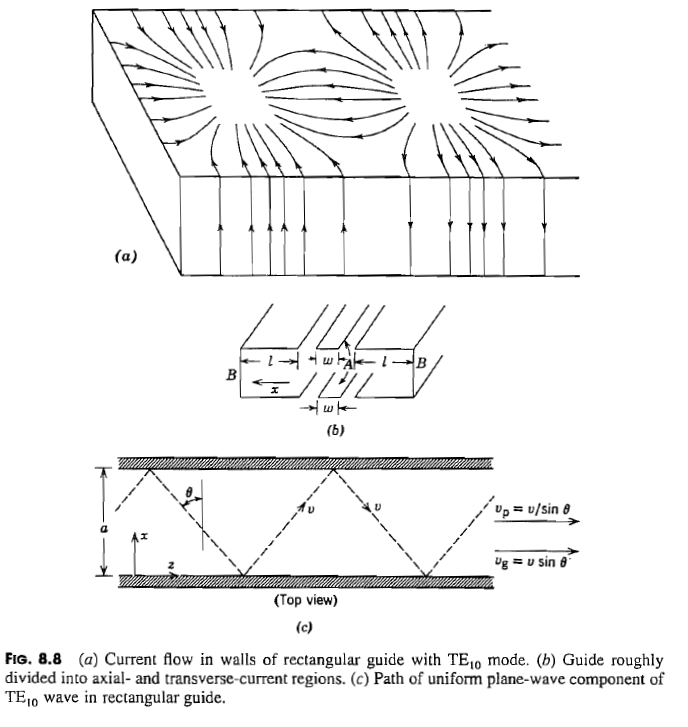
\includegraphics[scale= 0.9]{TE 10.PNG}
\end{figure}  

\newpage 

\section{Modo $TE_{20}$} 

\footnote{Slide del prof | PPT: Lezione 21 - 22 Guide rettangolari 22-24 maggio 2023 | Pag 40-42} 

Le guide d'onda sono dimensionate in modo tale che, alla frequenza di lavoro, 
ci sia solo un solo modo di propagazione, quindi: 

{
    \Large
    \begin{equation}
        a \ge 2b
    \end{equation}
}

La frequenza di cut-off per la $TE_{20}$ è: 

{
    \Large 
    \begin{equation}
        f_{c_{20}} [GHz] = \frac{300}{a [mm]}
    \end{equation}
}

Quindi l'intervallo di monomodalità, cioè l'intervallo di frequenze in cui l'onda si può propagare 
nel sistema guida d'onda così progettato è di: 

{
    \Large 
    \begin{equation}
        \frac{300}{a [mm]} \ge f[GHz] \ge \frac{150}{a [mm]}
    \end{equation}
} 

Se $m=0$, la guida d'onda non dipende da b. \\ 

$\omega_{c_{n0}}$ aumenta al diminuire di b. \\ 

Quindi b può essere il più piccolopossibile. \\ 

Ma il campo max è inversamente proporzionale a $\sqrt{b}$ 

{
    \Large 
    \begin{equation}
        \alpha_c \approx 
        \frac{R_s}{a^{3} b \kappa \eta} (2b\pi^{2} + a^{3} \kappa^{2})
    \end{equation}
}

dove: 

{
    \Large 
    \begin{equation}
        R_s = \frac{1}{\sigma \delta}
    \end{equation}
}


Quindi tipicamente: 

{
    \Large
    \begin{equation}
        a \approx 2b
    \end{equation}
}

\newpage 


\end{document}